\chapter{Results}\label{results}

In this chapter, we analyze two proposed idealized models of the TCPC. These models are designed to incorporate key geometric modifications identified as beneficial in reducing energy dissipation, as described in \cite{Rijnberg2018}. These modifications, summarized in Figure~\ref{fig:positive_modifications}, serve as a foundation for investigating the effects of caval offsetting, curving, flaring, and other geometric factors on flow dynamics.

\begin{figure}[H]
	\centering
	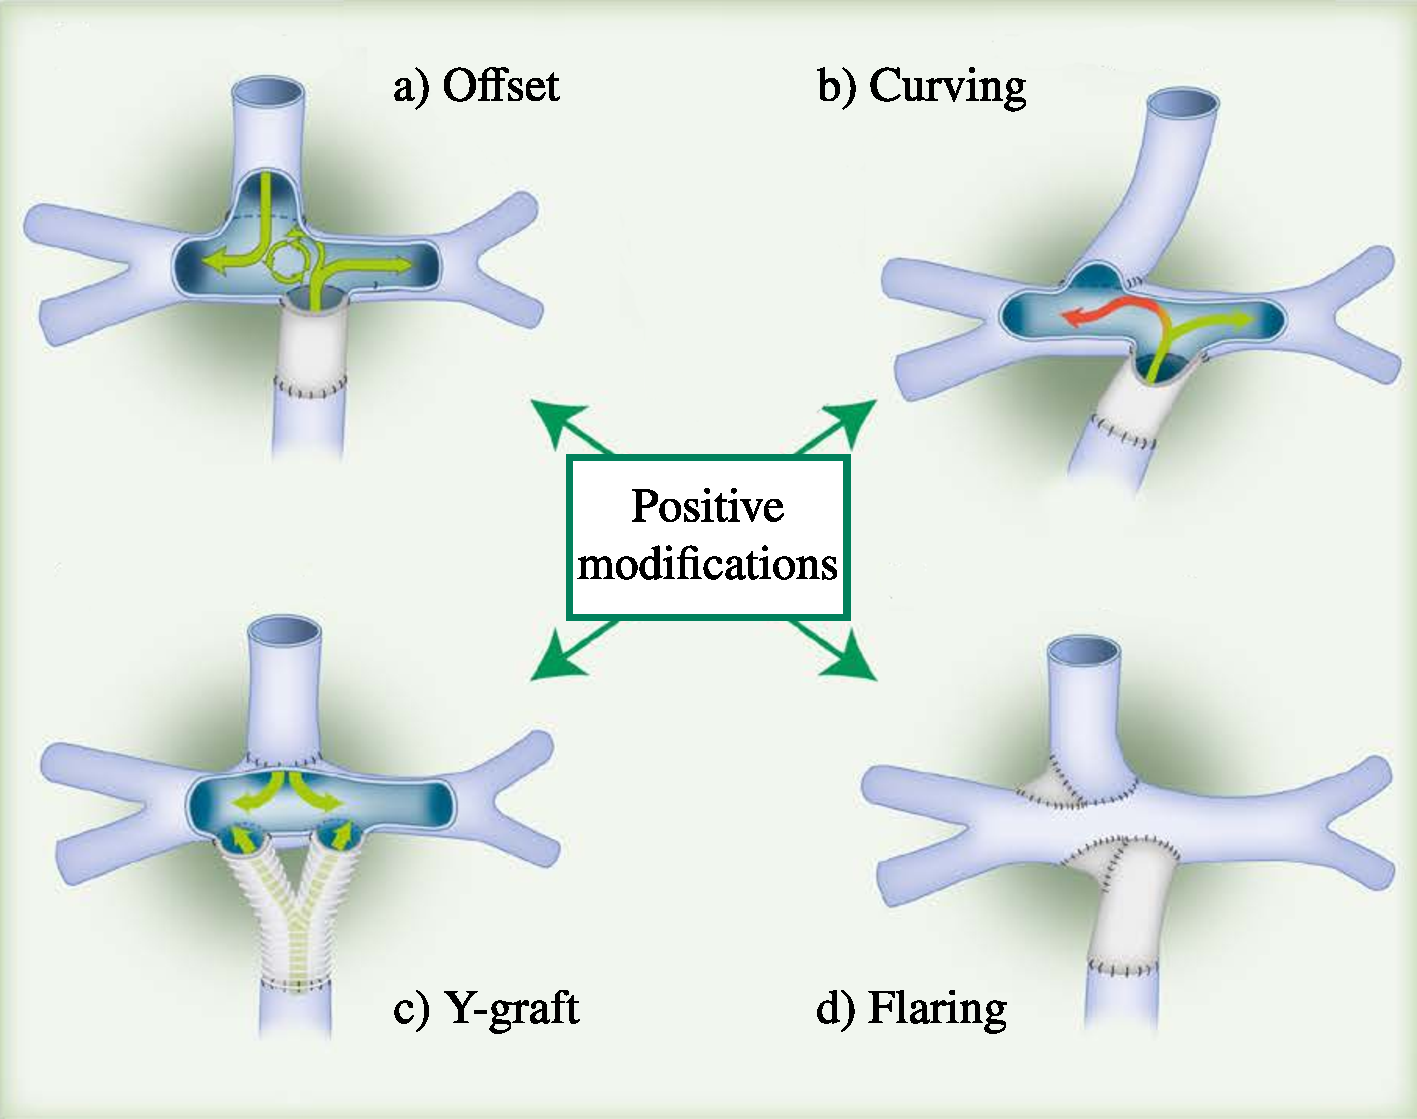
\includegraphics[width=0.65\textwidth]{figures/energyloss-en.pdf}
	\caption[Positive Modifications for TCPC]{Key modifications to improve TCPC geometry and reduce energy dissipation: (a) caval offsetting, where the inferior and superior vena cava are misaligned to minimize flow collision; (b) curving, where the conduits are curved to enhance flow alignment; (c) the Y-graft configuration, which splits the flow evenly between outlets; and (d) flaring, where the connections are widened to reduce sharp corners and flow resistance. Adapted from \cite{Rijnberg2018}.}
	\label{fig:positive_modifications}
\end{figure}

\section{The Models}

To systematically evaluate the effects of geometric changes, the models were developed with varying levels of complexity, incorporating different numbers of degrees of freedom. Both models represent idealized TCPC geometries and share the same labeling convention for inlets and outlets. Specifically, the inlets are denoted as $\Gamma^{N}_{\text{in}}$ (top inlet representing the superior vena cava) and $\Gamma^{S}_{\text{in}}$ (bottom inlet representing the inferior vena cava with the conduit). The outlets are labeled as $\Gamma^{W}_{\text{out}}$ (left outlet representing the left pulmonary artery) and $\Gamma^{E}_{\text{out}}$ (right outlet representing the right pulmonary artery). The shared geometric framework, along with labeled boundaries, is illustrated in Figure~\ref{fig:junction schema}.

\begin{figure}[H]
	\centering
	\begin{subfigure}{0.45\textwidth}
		\centering
		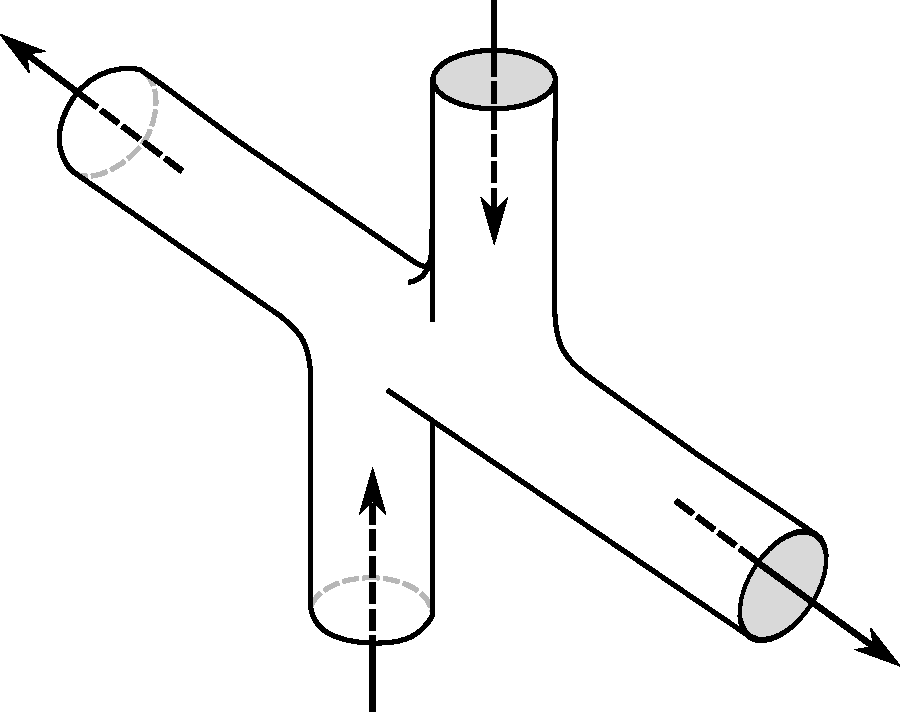
\includegraphics[width=0.75\textwidth, trim={0mm -13mm 0mm 0mm}]{figures/3dschema.pdf}
		\caption{3D schematic of the idealized TCPC junction.}
		\label{fig:schema 3d}
	\end{subfigure}\hspace{2mm}
	\begin{subfigure}{0.53\textwidth}
		\centering
		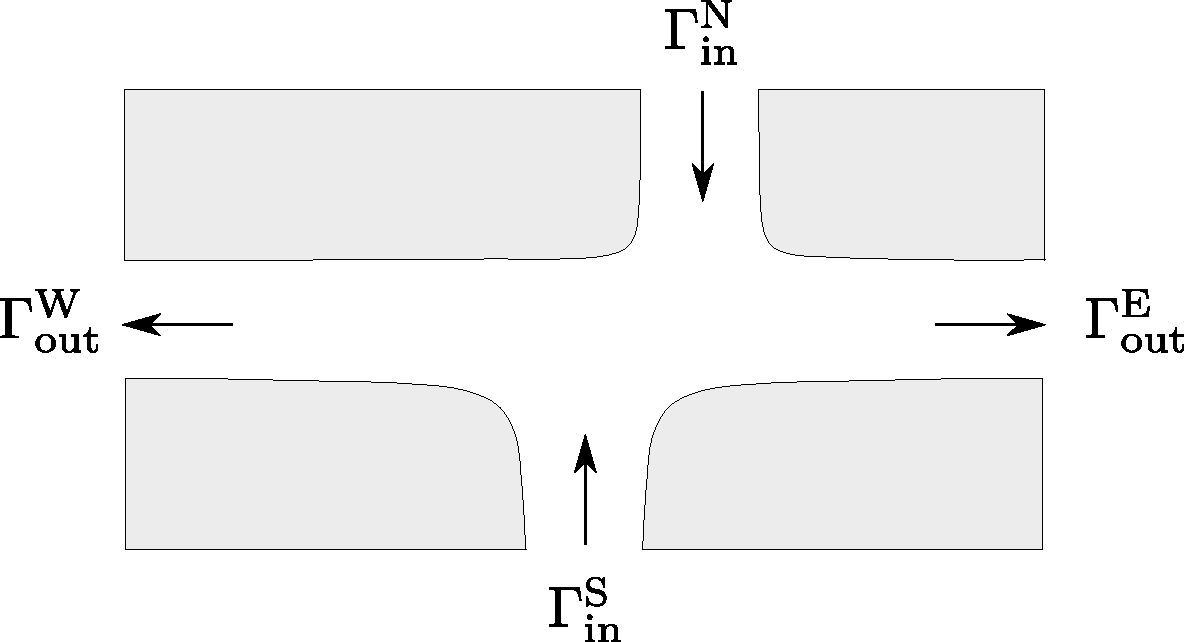
\includegraphics[width=0.99\textwidth, trim={0mm -5mm 0mm 0mm}]{figures/2dschema.pdf}
		\caption{2D schematic of the idealized TCPC junction, highlighting labeled boundaries.}
		\label{fig:schema 2d}
	\end{subfigure}
	\vspace{2mm}
	\caption[Schematic of Idealized TCPC Geometry]{2D and 3D schematic illustrations of the idealized TCPC geometry, showing labeled inlets ($\Gamma^{N}_{\text{in}}$, $\Gamma^{S}_{\text{in}}$) and outlets ($\Gamma^{W}_{\text{out}}$, $\Gamma^{E}_{\text{out}}$).}
	\label{fig:junction schema}
\end{figure}


\subsection{Model 1: Simplified Cylindrical Junction}

The first model represents a basic cylindrical junction, where the bottom vertical cylinder corresponds to the inferior vena cava (IVC), the horizontal cylinder corresponds to the pulmonary artery, and the top vertical cylinder represents the superior vena cava (SVC). The IVC and SVC are connected perpendicularly to the pulmonary artery, creating a cross-like structure. 

Model 1 was chosen because it introduces only one degree of freedom: the vertical offset of the IVC relative to the SVC. This simplicity makes it feasible to sample and evaluate the optimization space exhaustively, providing an opportunity to study the behavior of the objective functions, namely wall shear stress (WSS) and turbulence kinetic energy (TKE), in detail.

\begin{figure}[H]
	\centering
	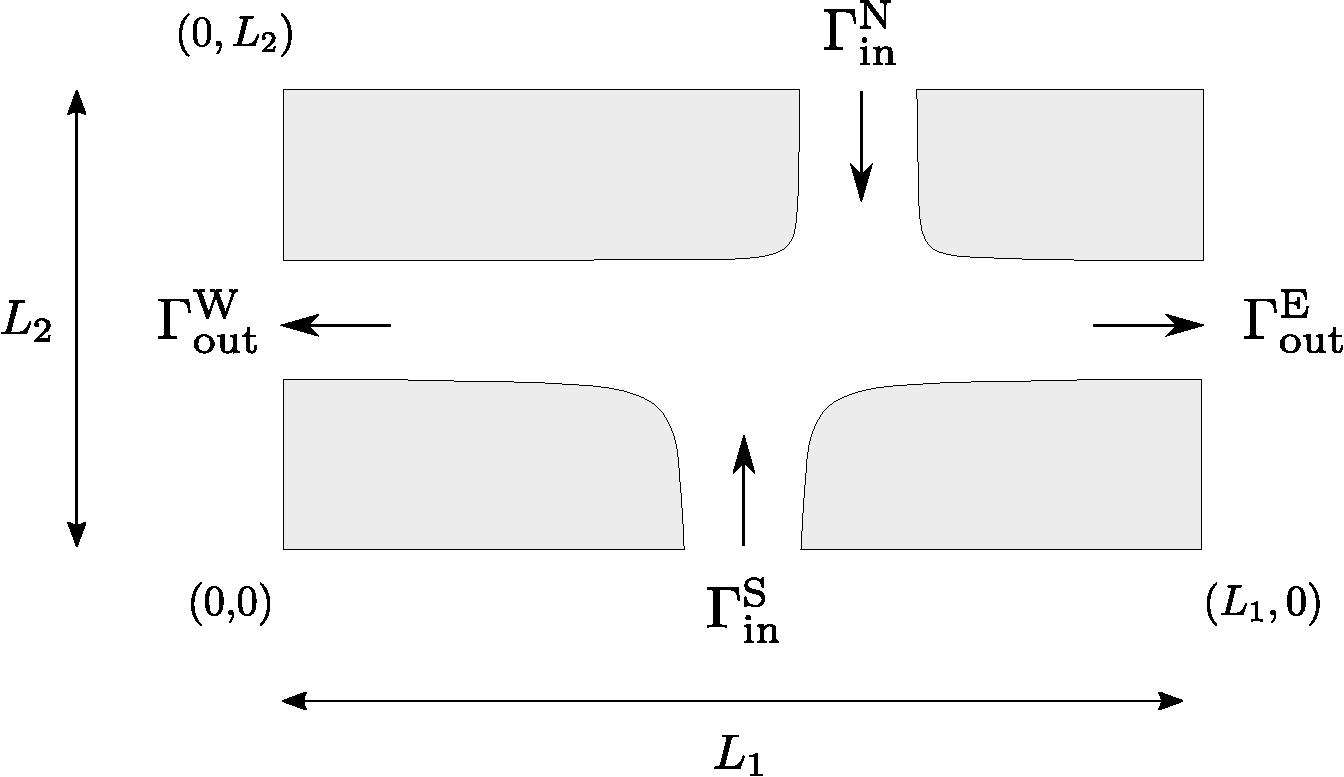
\includegraphics[width=0.8\textwidth]{figures/krizovatka-obecna.pdf} % Replace with your figure for Model 1
	\caption[Simplified Cylindrical Junction]{Schematic of Model 1: A simplified cylindrical junction with one degree of freedom, the vertical offset of the IVC relative to the SVC.}
	\label{fig:model1_schematic}
\end{figure}

\subsection{Model 2: Complex Geometric Model}

The second model introduces additional complexity by incorporating five degrees of freedom: the vertical offset of the IVC, the angles of connection for both the IVC and SVC to the pulmonary artery, the flaring of the IVC, and the width of the IVC. This model enables a more detailed investigation of the interaction between geometric parameters and hemodynamic efficiency.

Model 2 was selected because its higher complexity allows for greater variations in geometry and, consequently, a potentially larger impact on flow dynamics. However, the increased number of degrees of freedom makes it infeasible to sample the optimization space comprehensively, rendering the model more akin to a "black box" during optimization.

\begin{figure}[H]
	\centering
	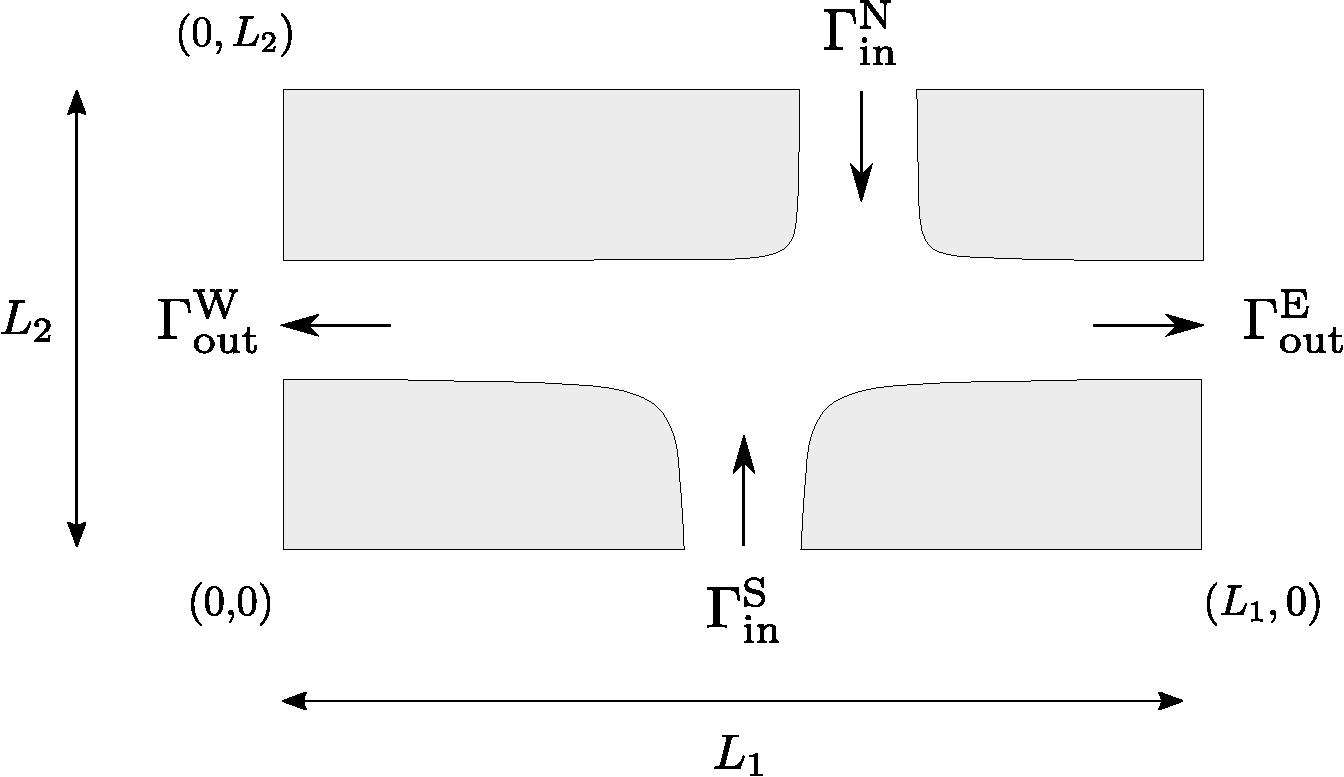
\includegraphics[width=0.8\textwidth]{figures/krizovatka-obecna.pdf} % Replace with your figure for Model 2
	\caption[Complex Geometric Model]{Schematic of Model 2: A more complex model with five degrees of freedom—IVC offset, connection angles, flaring, and width of the IVC.}
	\label{fig:model2_schematic}
\end{figure}

\section{Objective functions and other monitored quantities}
Selecting appropriate objective functions is essential for guiding geometric optimization. In this work, we focus primarily on two such functions: the turbulence kinetic energy (TKE) and the shear rate near the walls. In addition, we also present other relevant metrics that are monitored during the computations.

\subsubsection*{Turbulence kinetic energy}
TKE, defined by~\eqref{eq:turb kin energy}, measures the intensity of velocity fluctuations within the flow. In the context of the TCPC, higher TKE generally corresponds to increased energy losses. Thus, reducing TKE in the TCPC region is desirable in order to improve hemodynamic efficiency. We sum TKE over a defined control volume within the computational domain, obtaining a global level of turbulent activity in the region. In the case of TCPC, TKE can serve as surrogate measure of how smoothly and efficiently blood flows through the connection.

\subsubsection*{Shear rate}
Shear rate, defined in \eqref{eq:dot gamma}, provides insight into the mechanical forces acting on the vessel walls. Excessive shear rate can negatively affect the vascular health, making controlling near-wall shear rates crucial for ensuring the long-term patency and physiological compatibility of the TCPC.

However, measuring shear rate directly at the wall in a computational framework -- especially using LBM -- poses a challenge. The discrete nature of the grid and the no-slip boundary condition mean that the resolution near the wall can affect the computed shear rate and make it sensitive to discretization details. To address this, we introduce a thin layer of thickness 1 mm adjacent to the vessel walls. Within this layer, we sum the shear rate values rather than relying solely on the cells immediately neighboring the walls. This approach was chosen to reduce the sensitivity on grid characteristics while maintaining the physiological relevance of the quantity, ensuring it provides representative measure of local flow behavior.

\subsubsection*{IVC flow split}
In addition to the main objective functions, we monitor how fluid from the inferior vena cava divides between the left and right pulmonary arteries. A balanced or at least minimally maintained split of inferior vena cava flow into both pulmonary artery branches is desirable. This metric is evaluated in post-processing using the computed mean velocity field.

\subsubsection*{Mean velocity vector angle at the pulmonary artery outlets}
It is beneficial for blood in the pulmonary arteries to flow downstream in a laminar manner. Thus, we examine the angle between the mean velocity vector and the outlet normal vector. This angle provides the information  for studying the laminarity of the flow.

\section{The models}

To systematically evaluate the effects of geometric changes, the models were developed with varying levels of complexity, incorporating different numbers of degrees of freedom. Both models represent idealized TCPC geometries and share the same labeling convention for inlets and outlets. 

The inlets are denoted as $\Gamma^{\text{N}}_{\text{in}}$ (representing the superior vena cava at the top) and $\Gamma^{\text{S}}_{\text{in}}$ (representing the inferior vena cava with the conduit at the bottom). Similarly, the outlets are labeled as $\Gamma^{\text{W}}_{\text{out}}$ (representing the left part of the pulmonary artery) and $\Gamma^{\text{E}}_{\text{out}}$ (representing the right part of the pulmonary artery).
The shared geometric framework and boundary labels, is illustrated in Figure~\ref{fig:junction schema}. The dimensions of cylindrical segments forming the simplified junction are presented in Table~\ref{tab:tcpc dims}.


\begin{figure}[H]
	\centering
	\vspace{2mm}
	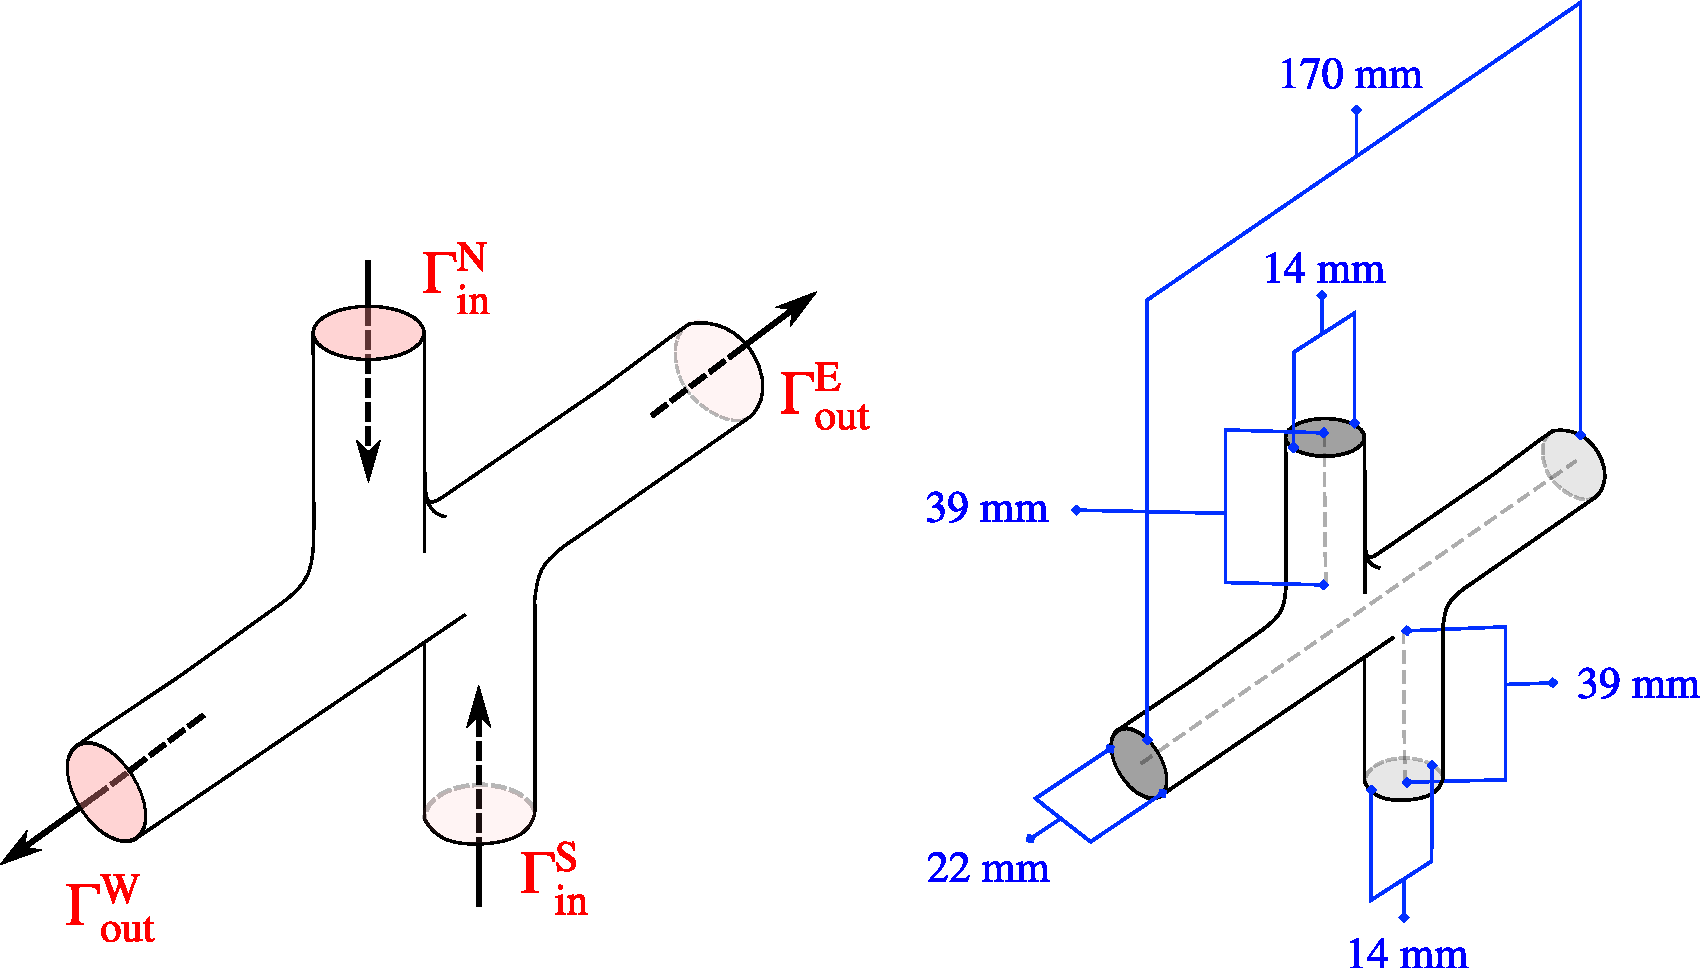
\includegraphics[width=0.99\textwidth]{figures/3d-tcpc-schema-combined.pdf}
	\vspace{7mm}
	\caption{Schematic representation of the idealized TCPC geometry. The labeled inlets ($\Gamma^{\text{N}}_{\text{in}}$, $\Gamma^{\text{S}}_{\text{in}}$) and outlets ($\Gamma^{\text{W}}_{\text{out}}$, $\Gamma^{\text{E}}_{\text{out}}$), directions of inflows and outflows, and the dimensions of the cylindrical segments forming the junction are illustrated.}
	\label{fig:junction schema}
\end{figure}

\bgroup
\centering
\vspace{4mm}
\setlength\tabcolsep{3mm}
\def\arraystretch{1.7}%
\begin{tabular}{|l|l|c|c|}
	\hline
	Segment & Abbreviation & Length & Diameter \\ \hline
	Inferior vena cava 	& IVC 	&      39 mm        &     14 mm    \\ 
	Superior vena cava  & SVC 	&      39 mm     	&     14 mm     \\ 
	Pulmonary artery 	& PA 	&      170 mm     	&     22 mm     \\  \hline
\end{tabular}
\vspace{2mm}
\captionof{table}{Dimensions of the cylindrical segments forming the idealized TCPC junction.}
\vspace{4mm}
\label{tab:tcpc dims}
\egroup

In both models, the objective functions are studied within a defined control volume, denoted as A, which is a subset of the entire computational domain. By restricting the analysis to this region, we aim reduce potential errors introduced by the numerical boundary conditions. The control volume involves inlet and outlet boundaries named according to their respective vessel segments: \(\Gamma^{\text{SVC}}_{\text{in}}\) for the superior vena cava inlet, \(\Gamma^{\text{IVC}}_{\text{in}}\) for the inferior vena cava inlet, \(\Gamma^{\text{LPA}}_{\text{out}}\) for the left pulmonary artery outlet, and \(\Gamma^{\text{RPA}}_{\text{out}}\) for the right pulmonary artery outlet. The turbulence kinetic energy is evaluated in the entire control volume. The near-wall shear rate is examined along the boundaries of the control volume that are shared with the vessel walls.

\subsection*{Model 1: Simplified cylindrical junction}\label{mod:model1}
The first model represents a basic cylindrical junction where the IVC and SVC are connected perpendicularly to the PA, forming a cross-like structure, as illustrated in Figure~\ref{fig:model1_schematic}. Model 1 was chosen because it introduces only one degree of freedom, the horizontal offset of the IVC axis relative to the SVC, denoted by $o_1$. This simplicity makes it possible to sample the optimization space and evaluate the objective functions at the points of the sampling. This provides an opportunity to examine the behavior of the objective functions and verify the result generated by the optimization framework.

\subsection*{Model 2: More complex geometric model}\label{mod:model2}
Illustration of Model 2 is presented in Figure~\ref{fig:model1_schematic}. The second model introduces additional complexity by incorporating six degrees of freedom:
\begin{itemize}
	\item horizontal offset of the IVC axis, denoted by $o_1$,
	\item angle of the IVC axis, denoted by $\alpha_1$,
	\item angle of the SVC axis, denoted by $\alpha_2$,
	\item width and curvature of the IVC-PA connection, denoted by $f_1$,
	\item width and curvature of the SVC-PA connection, denoted by $f_2$,
	\item width of the IVC, denoted by $l_1$.
\end{itemize}
Model 2 was selected because its higher complexity allows for more geometric variations.

\begin{figure}[H]
	\begin{subfigure}{0.48\textwidth}
		\centering
		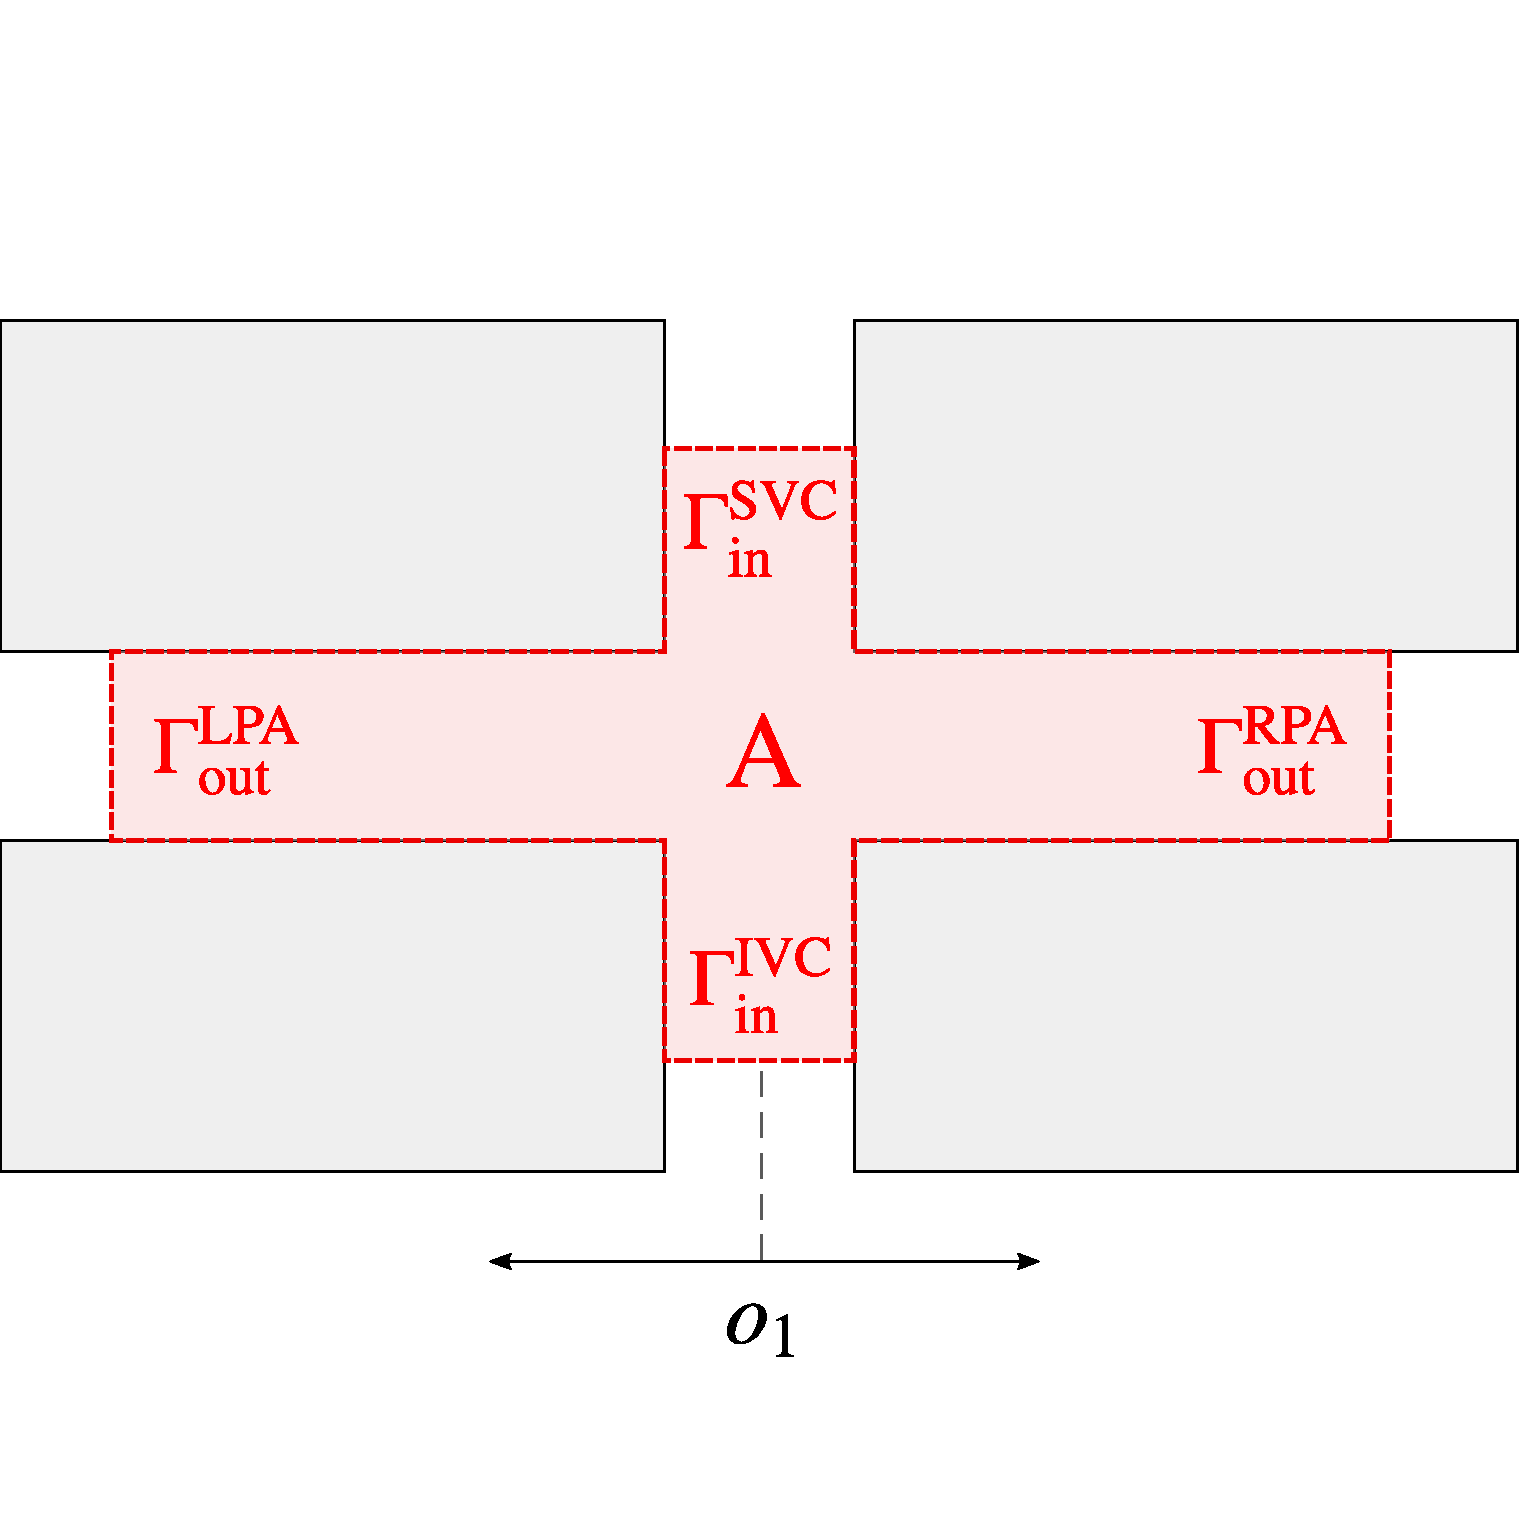
\includegraphics[width=0.91\textwidth, trim={0 0 0 0}]{figures/model1.pdf}
		\caption[Simplified Cylindrical Junction]{Schematic of Model 1: A simplified cylindrical junction with one degree of freedom, the horizontal offset of the IVC.}
		\label{fig:model1_schematic}
	\end{subfigure}\hfill%
	\begin{subfigure}{0.48\textwidth}
		\centering
		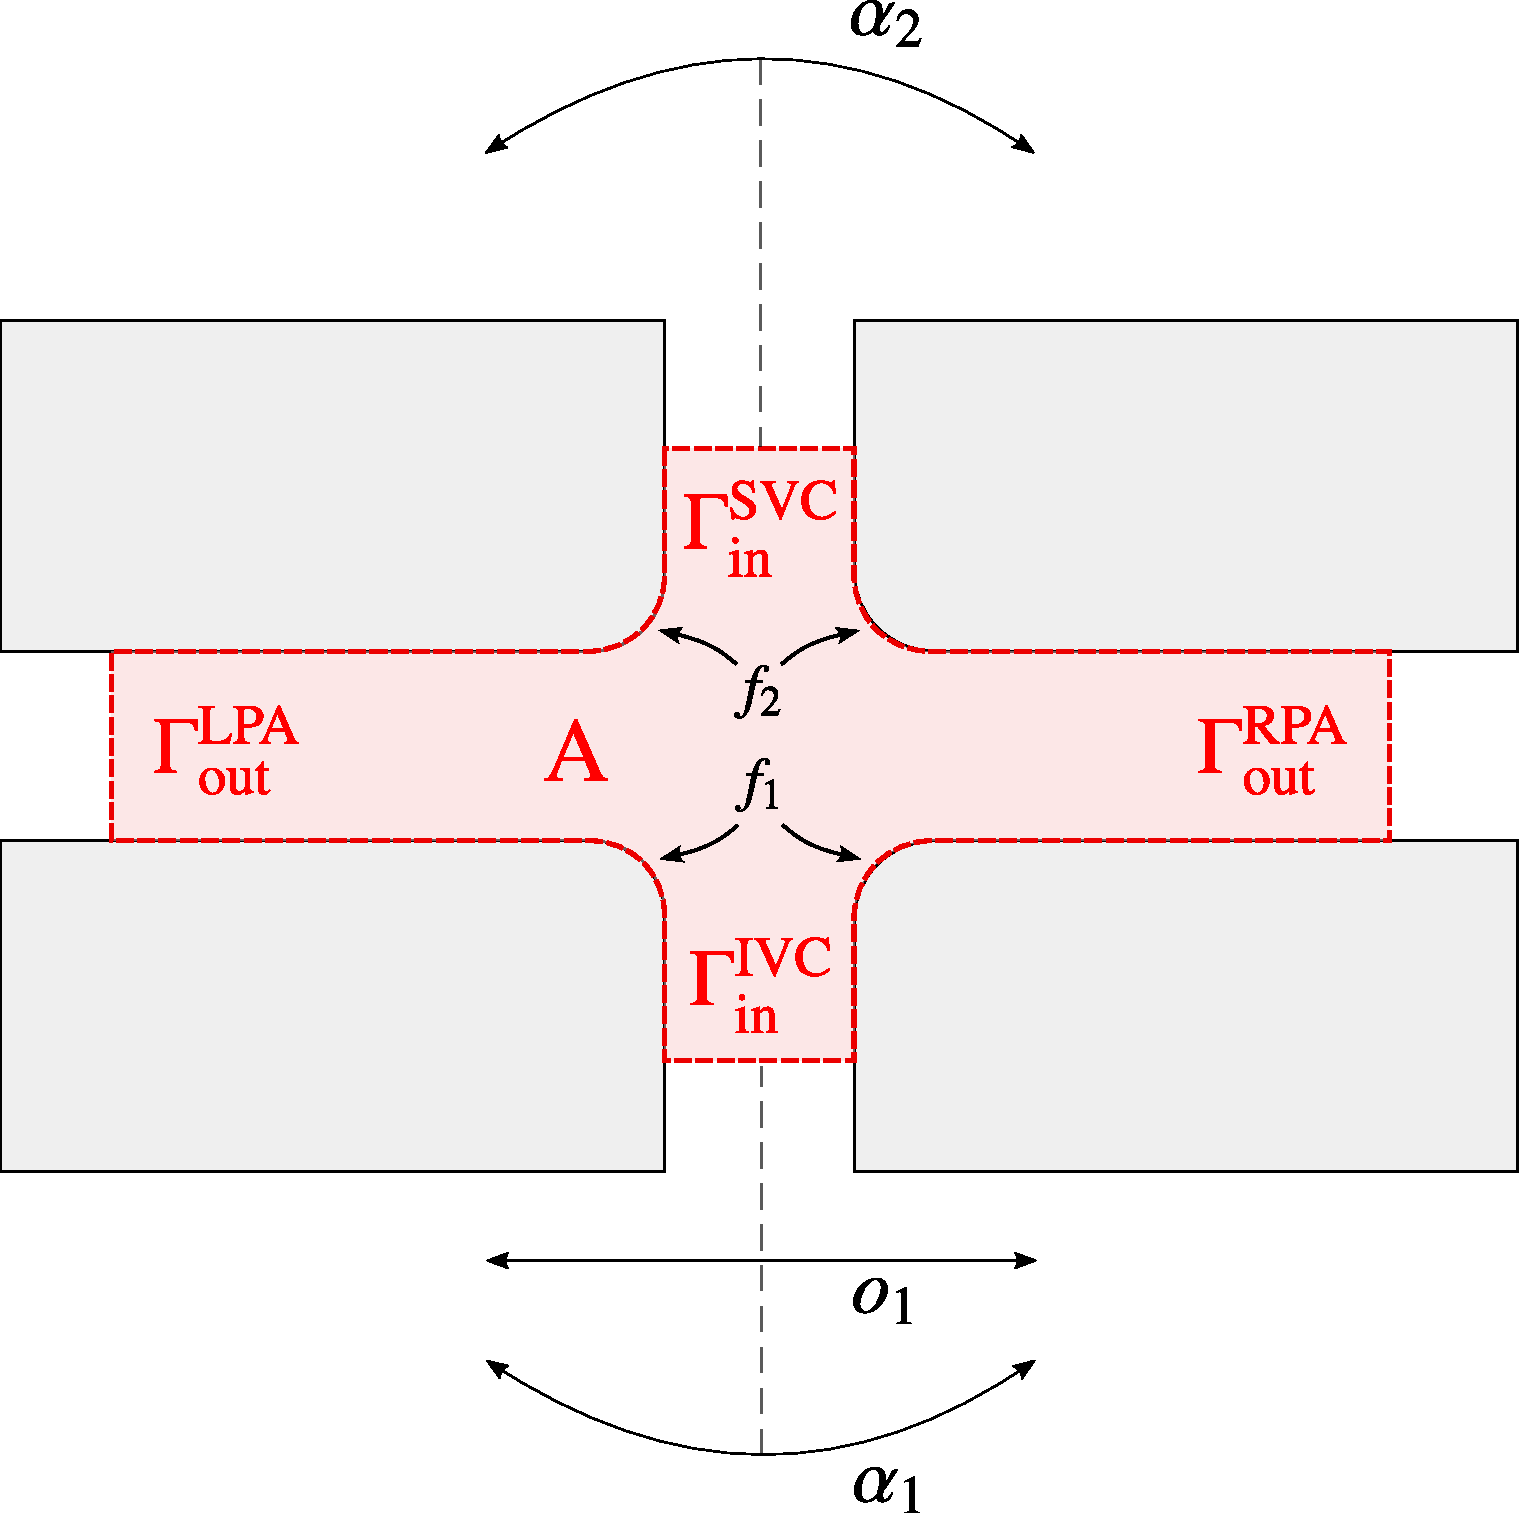
\includegraphics[width=0.91\textwidth]{figures/model2.pdf}
		\caption[Complex Geometric Model]{Schematic of Model 2: A more complex model introducing six degrees of freedom: IVC offset and width, connection angles and flaring.}
		\label{fig:model2_schematic}
	\end{subfigure}
	\vspace{4mm}
	\caption{Schematic illustrations of Model 1 and Model 2.}
	\label{fig:model schemas}
\end{figure}
\section{Problem with one optimization parameter}\label{optim1}
In this section, we focus on a simplified model of the TCPC in a form of a basic cylindrical junction to investigate the behavior of key hemodynamic quantities under varying caval offset. The problem setup is defined in Problem Setup \hyperlink{page.48}{1}. The dimensions of the domain, the value of the kinematic viscosity, and the value of the inflows are chosen to mimic real values occurring in physiological conditions \cite{Rijnberg2018}.

\vspace{2mm}
\begin{problem}{Basic cylindrical junction}
	\vspace{2mm}
	Physical setup:
	\begin{itemize}
		\item Domain: $ \Omega=(0 ; 170 \mathrm{~mm}) \times(0 ; 22 \mathrm{~mm}) \times(0 ; 100 \mathrm{~mm})$.
		\item Kinematic viscosity: $ \nu=3 \cdot 10^{-6} \mathrm{~m}^{2} \mathrm{~s}^{-1}$.
		\item Inflow at $\Gamma^{\text{IVC}}_{\text{in}}$: a constant velocity of magnitude $0{,}45$ \si{m s^{-1}},  aligned with the IVC axis in the positive $x_3$-direction.
		\item Inflow at $\Gamma^{\text{SVC}}_{\text{in}}$: a constant velocity of magnitude $0{,}35$ \si{m s^{-1}}, aligned with the SVC axis in the negative $x_3$-direction.
	\end{itemize} 
	LBM setup:
	\begin{itemize}
		\item Initial condition on $ \overline{\hat{\Omega}} $ set as described in Section~\ref{pocatecni podminka}.
		\item Boundary conditions at $\Gamma^{\text{W}}_{\text{out}}$ and $\Gamma^{\text{E}}_{\text{out}}$ set according to Section~\ref{symmetric bc}.
		\item Discretization: $\overline{\hat{\Omega}} = N_{x} \times N_{y} \times N_{z}$, $N_{x} = 768, \, N_{y} = 105, N_{z} = 453$.
		\item Kinematic viscosity in lattice units: $\nu^{L} = 10^{-3} $.
	\end{itemize}
	
\end{problem}

\subsection{Analysis of the system}
The main objective of this study is to minimize two studied quantities, $\dot{\gamma}^{A}_{\mathrm{nw}}$ and $T^{A}_{\mathrm{turb}}$. To study the system's behavior and to validate the result generated by the optimization framework, we systematically sample the optimization space prior to running the optimization algorithm.

Specifically, we discretize the $o_1$-parameter space with regular intervals of $0{,}1$ cm over the range $[0{,}1 \, \mathrm{cm}; 2{,}4 \, \mathrm{cm}]$, creating a set of sampling points
\begin{equation}
	P = \Big\{ \, \text{P}_i \, \big| \, i=0,1,2, \dots, 24 \, \Big\} = \Big\{ \, 0{,}1 \cdot i \: \big| \, i=0,1,2, \dots, 24 \, \Big\} \, .
\end{equation}
At each point of $P$, the system's response is evaluated by computing different flow characteristics. This study serves two purposes:
\begin{itemize}
	\item It provides insight into the system's behavior. Studying different geometrical setups helps with understanding of how flow characteristics vary with the changing value of parameter~$o_1$.
	\item By analyzing the sampled data, we can validate the performance of the optimization framework.
\end{itemize}
The results of the functions evaluations in the points of sampling are presented in Figure~\ref{fig:summary_metrics}.


\newgeometry{top=4.0cm}
\begin{figure}[H]
	\centering
	\begin{subfigure}{0.49\textwidth}
		\centering
		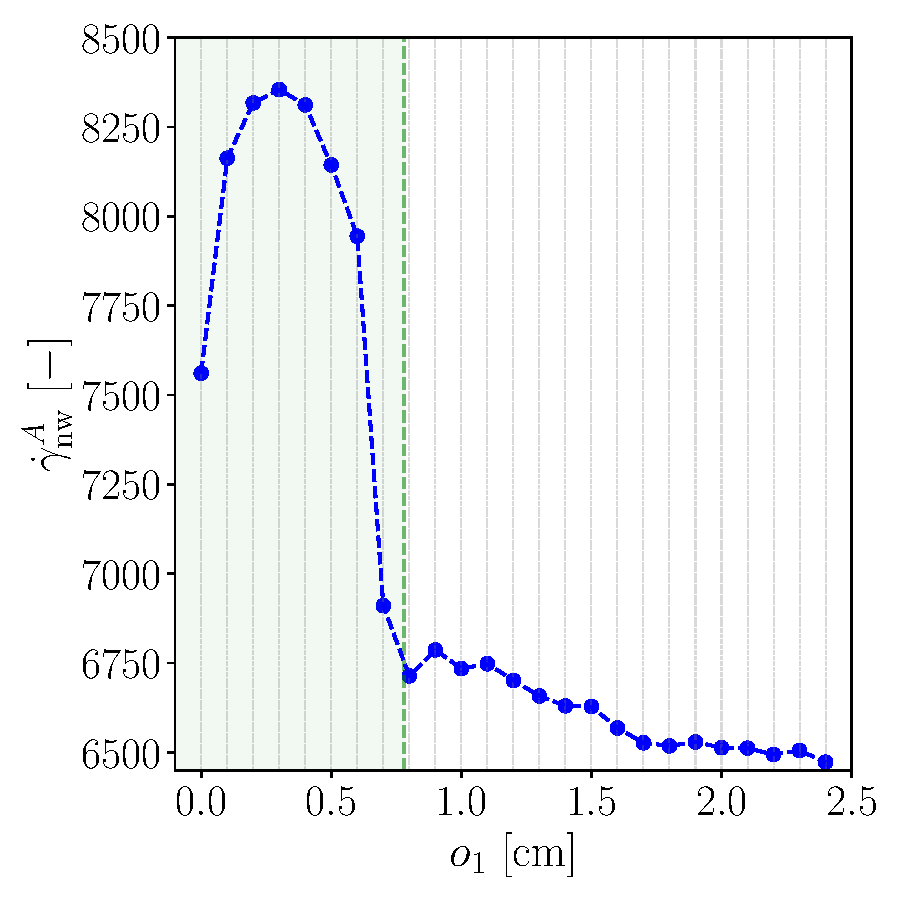
\includegraphics[
		width=\textwidth,
		trim={0mm 0mm 0mm 0mm}
		]{figures/mean_stress_3_interpolated.pdf}
		\caption{Near-wall shear rate ($\dot{\gamma}^{A}_{\mathrm{nw}}$) in lattice units, with the green region indicating flow from the IVC exceeding~25\%.}
		\label{fig:shear_rate}
	\end{subfigure}\hfill%
	\begin{subfigure}{0.49\textwidth}
		\centering
		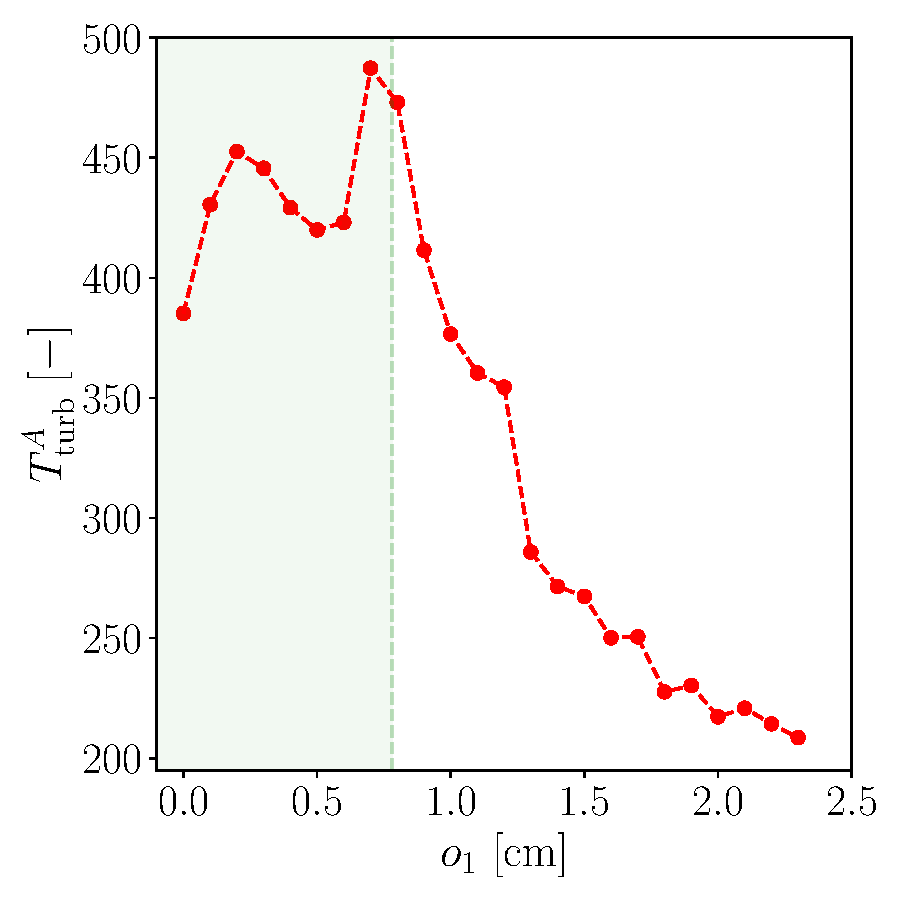
\includegraphics[
		width=\textwidth,
		trim={0mm 0mm 0mm 0mm}
		]{figures/mean_turbulence_kinetic_energy_interpolated.pdf}
		\caption{Turbulent kinetic energy ($T^{A}_{\mathrm{turb}}$) in lattice units, with the green region indicating flow from the IVC exceeding~25\%.}
		\label{fig:tke}
	\end{subfigure}
	\\[10pt]
	\begin{subfigure}{0.49\textwidth}
		\centering
		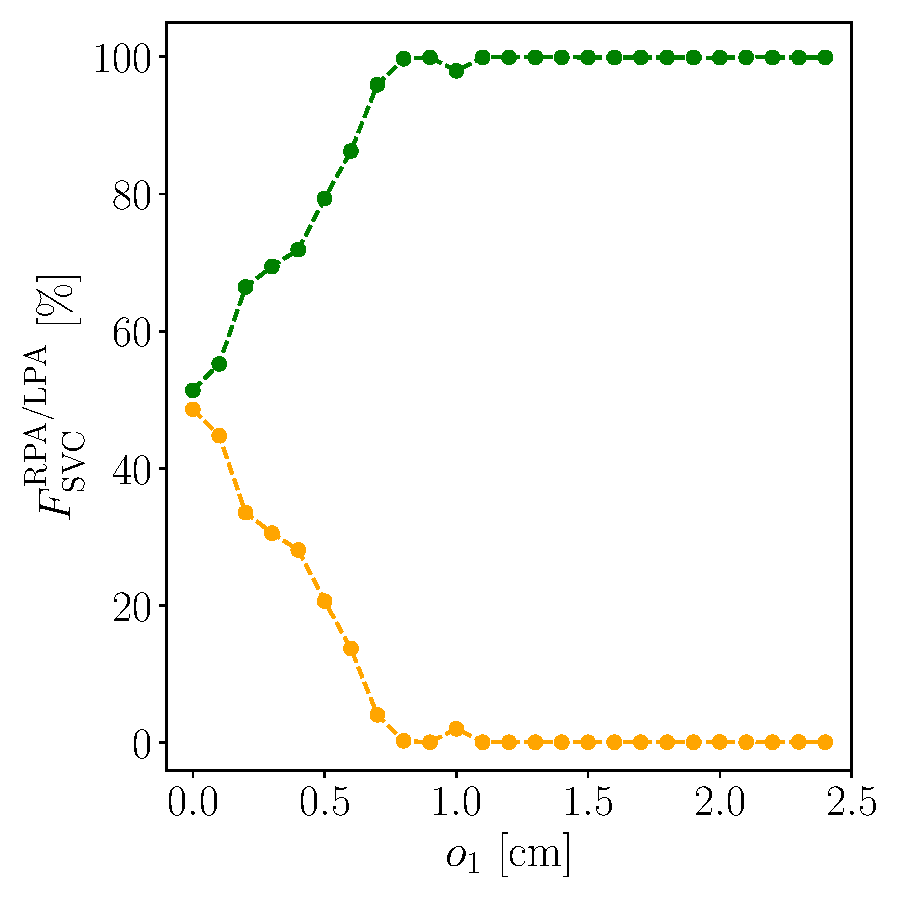
\includegraphics[
		width=\textwidth,
		trim={0mm 0mm 0mm 0mm}
		]{figures/svc_lpa.pdf}
		\vspace{4mm}
		\caption{Percentage of flow directed from the SVC to the LPA (green dashed line) and RPA (orange dashed line).}
		\label{fig:svc_flow_split}
	\end{subfigure}\hfill%
	\begin{subfigure}{0.49\textwidth}
		\centering
		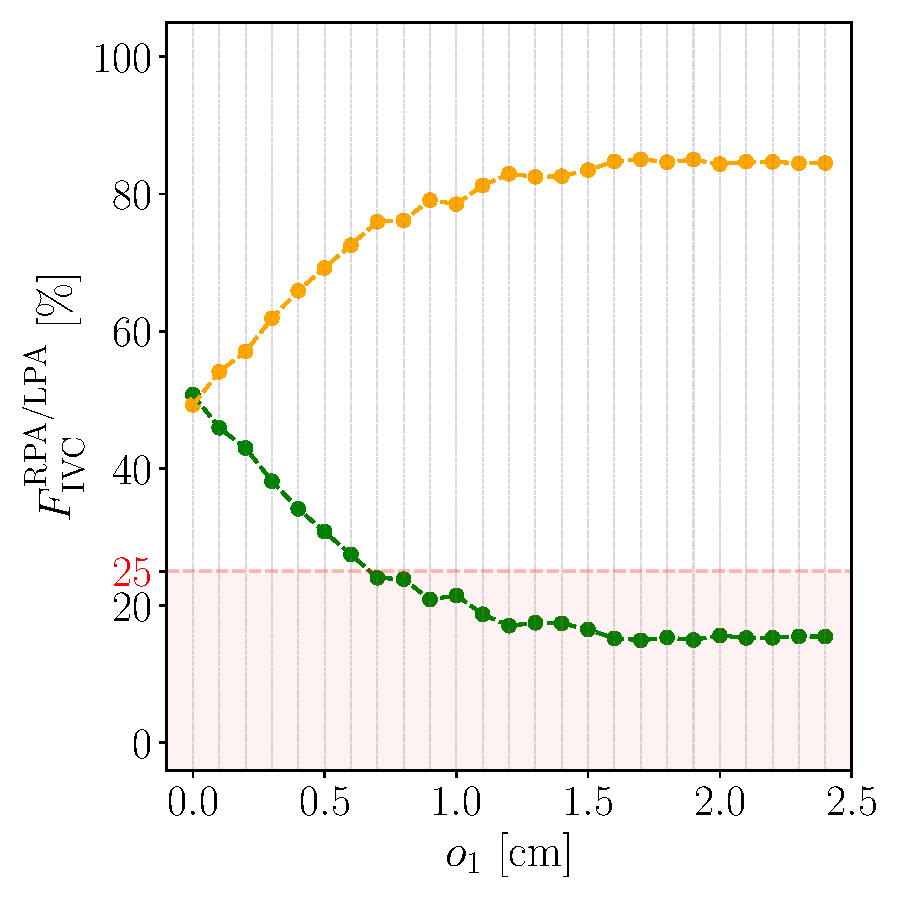
\includegraphics[
		width=\textwidth,
		trim={0mm 0mm 0mm 2.0mm}
		]{figures/ivc_lpa.pdf}
		\vspace{5mm}
		\caption{Percentage of flow directed from the IVC to the LPA and RPA. The red region highlights offsets where the flow fraction to the LPA is below 25\%.}
		\label{fig:ivc_flow_split}
	\end{subfigure}
	\begin{center}
		\vspace{-30mm}
		
\includegraphics[
		width=0.25\textwidth,
		trim={0mm 0mm 0mm 0mm}
		]{figures/ivc-svc-leg.png}
		\vspace{20mm}
	\end{center}
	\vspace{2mm}
	\caption{Summary of key analyzed metrics. (a) Near-wall shear rate ($\dot{\gamma}^{A}_{\mathrm{nw}}$) in lattice units, with green region indicating offsets for which IVC-LPA flow exceeds 25\%; (b) Turbulent kinetic energy ($T^{A}_{\mathrm{turb}}$) in lattice units, with similar IVC-LPA flow threshold; (c) Flow distribution from the SVC to the LPA and the RPA; (d) Flow distribution from the IVC to the LPA and RPA, with the red region indicating offsets where IVC-LPA flow is below 25\%.}

	\label{fig:summary_metrics}
\end{figure}
\restoregeometry
\newpage

Figure~\ref{fig:shear_rate} shows the near-wall shear rate $\dot{\gamma}^{A}_{\mathrm{nw}}$ as a function of $o_1$. At~$o_1 = 0{,}0 \, \mathrm{cm}$, where the geometry is perfectly symmetric, the shear rate is comparatively lower than it is for slightly larger offsets. Notably, we can observe sharp decrease to a local minimum at~$o_1 = 0{,}7 \, \mathrm{cm}$, i.e., an offset almost equal to 0{,}5-diameter of the IVC.  Subsequently, the shear rate exhibits a slight increase and then steadily declines to minimal values at higher offsets--around 1{,}5-diameter of the IVC.

The turbulent kinetic energy $T^{A}_{\mathrm{turb}}$ is shown in Figure~\ref{fig:tke}. At $o_1 = 0{,}0 \, \mathrm{cm}$, the value is again lower compared to slightly larger offsets. The peak of the TKE occurs at $o_1 = 0{,}7 \, \mathrm{cm}$, i.e., at the offset equal to 0{,}5-diameter of the IVC. The values then steadily decrease with increasing offset.

Figure~\ref{fig:svc_flow_split} illustrates the percentage of flow from the SVC directed into the LPA and the RPA. At~$o_1 = 0{,}0 \, \mathrm{cm}$, the flow splits evenly between the LPA and RPA, reflecting the symmetry of the geometry. As the offset increases, the flow to the LPA steadily rises up to 100 \%, meaning the SVC blood flows exclusively toward the LPA. Conversely, the flow to the RPA steadily falls to 0 \%. 

The flow split from the IVC is presented in Figure~\ref{fig:ivc_flow_split}. At $o_1 = 0{,}0 \, \mathrm{cm}$, the flow splits evenly between the LPA and RPA. As the offset increases, the flow to the RPA steadily increases up to around 85 \%, where it eventually levels. As it was already described in Section \ref{objective funcs meaning}, a balanced or at least minimally maintained split of IVC blood to each pulmonary artery branch is desirable. A threshold of minimal acceptable percentage directed to either one of the parts of the pulmonary artery was set at 25 \%. The red shaded region in Figure~\ref{fig:ivc_flow_split} highlights offsets where the IVC flow fraction falls below 25 \%. This also determines a offsets considered as acceptable, i.e., those satisfying the aforementioned minimal IVC flow split. Such offsets are highlighted by the green shaded regions in Figure~\ref{fig:shear_rate} and Figure~\ref{fig:tke}.

To deepen our understanding of the system’s behavior, Table~\ref{tab:studied points} details four specific points of interest for which additional metrics and flow characteristics were examined. These points--P$_0$, P$_7$, P$_8$, P$_24$--represent notable points at the functions' behavior. The reason for why each one of the points were chosen for further examination are also detailed in Table~\ref{tab:studied points}.
\vspace{7mm}
\begin{table}[H]
	\bgroup
	\centering
	\setlength\tabcolsep{3mm}
	\def\arraystretch{2.2}%
	\begin{tabular}{|c|c|c|p{8cm}|}
		\hline
		\textbf{Point} & \boldmath{$o_1$} \textbf{[cm]} & \textbf{Pages} & \textbf{Reason for detailed investigation} \\ \hline
		P$_0$ & 0{,}0 & \hyperlink{page.51}{51--52} & Symmetrical geometry; local minima in both $\dot{\gamma}^{A}_{\mathrm{nw}}$ and $T^{A}_{\mathrm{turb}}$. \\ \hline
		P$_7$ & 0{,}7 & \hyperlink{page.53}{53--54} & Offset associated with the maximum $T^{A}_{\mathrm{turb}}$. \\ \hline
		P$_8$ & 0{,}8 & \hyperlink{page.55}{55--56} &  Offset associated with a local minimum in $\dot{\gamma}^{A}_{\mathrm{nw}}$. \\ \hline
		P$_{24}$ & 2{,}4 & \hyperlink{page.57}{57--58} & Large offset associated with minimal values of both $\dot{\gamma}^{A}_{\mathrm{nw}}$ and $T^{A}_{\mathrm{turb}}$. \\ \hline
	\end{tabular}
	 \caption{Key offset points selected for detailed analysis. Each point corresponds to notable extrema or special configurations of $\dot{\gamma}^{A}_{\mathrm{nw}}$ or $T^{A}_{\mathrm{turb}}$.}
	\label{tab:studied points}
	\egroup
\end{table}

\section*{Point P$_\mathbf{0}$($o_1=0{,}0 \, \mathrm{ cm}$)}
\begin{figure}[H]
	
	\subsection*{Mean velocities}
	\vspace{-3mm}
	\rule{\textwidth}{0.4pt}
	
	\begin{subfigure}{0.60\textwidth}
		\centering
		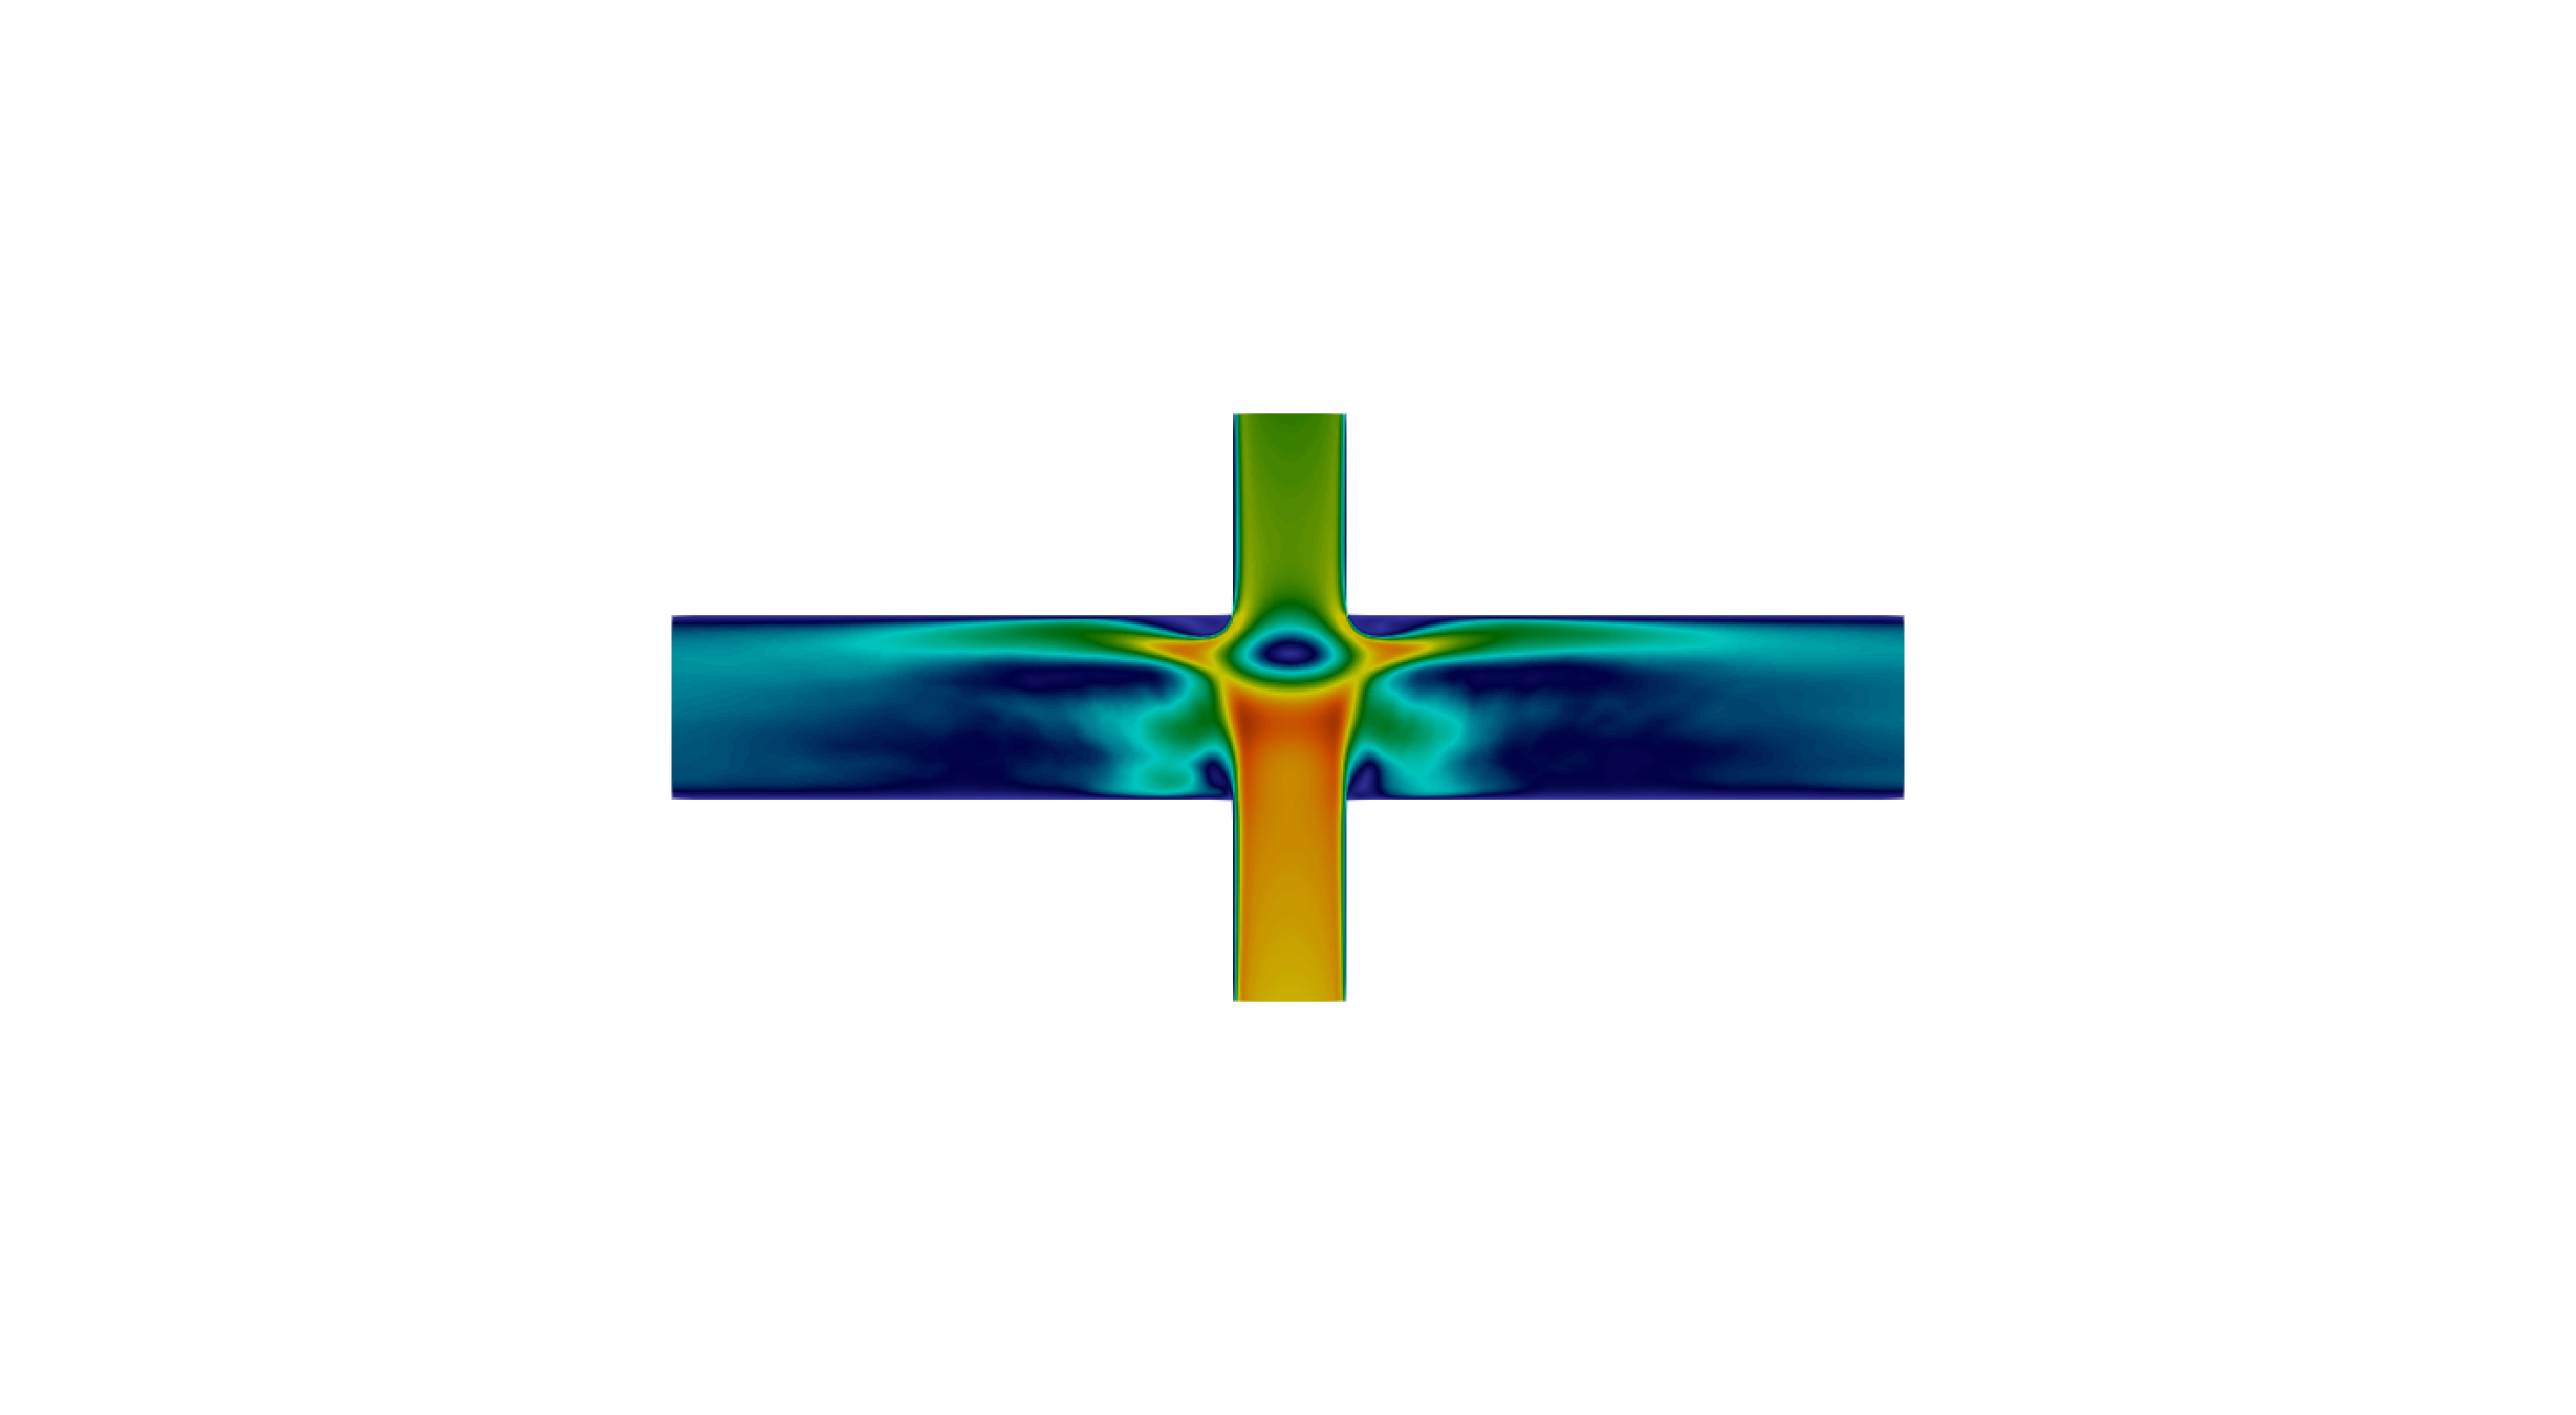
\includegraphics[
		width=\textwidth,
		trim={130mm 70mm 130mm 70mm},
		clip
		]
		{figures/plots/00/00_mean_veloc_xz.pdf}%
		\rlap{\hspace{-9.5cm}\raisebox{-0.0cm}{%  move next graphics to top right corner
				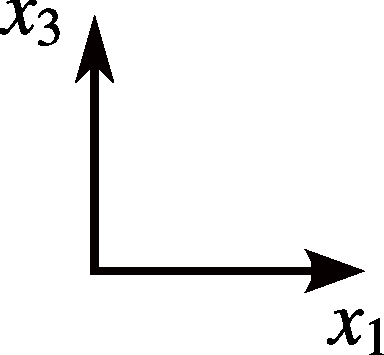
\includegraphics[height=1.5cm]{figures/x1x3.pdf}%
		}}
		
		
\includegraphics[
		width=0.85\textwidth,
		]
		{figures/plots/filler.pdf}
		\caption{Mean velocity magnitude field in the \(x_1\)-\(x_3\) plane.}
		\label{fig:mean_velocity_xz00}
		
	\end{subfigure}\hfill%
	\begin{subfigure}{0.36\textwidth}
		\vspace{14mm}
		\centering
		LPA\hspace{24mm}RPA
		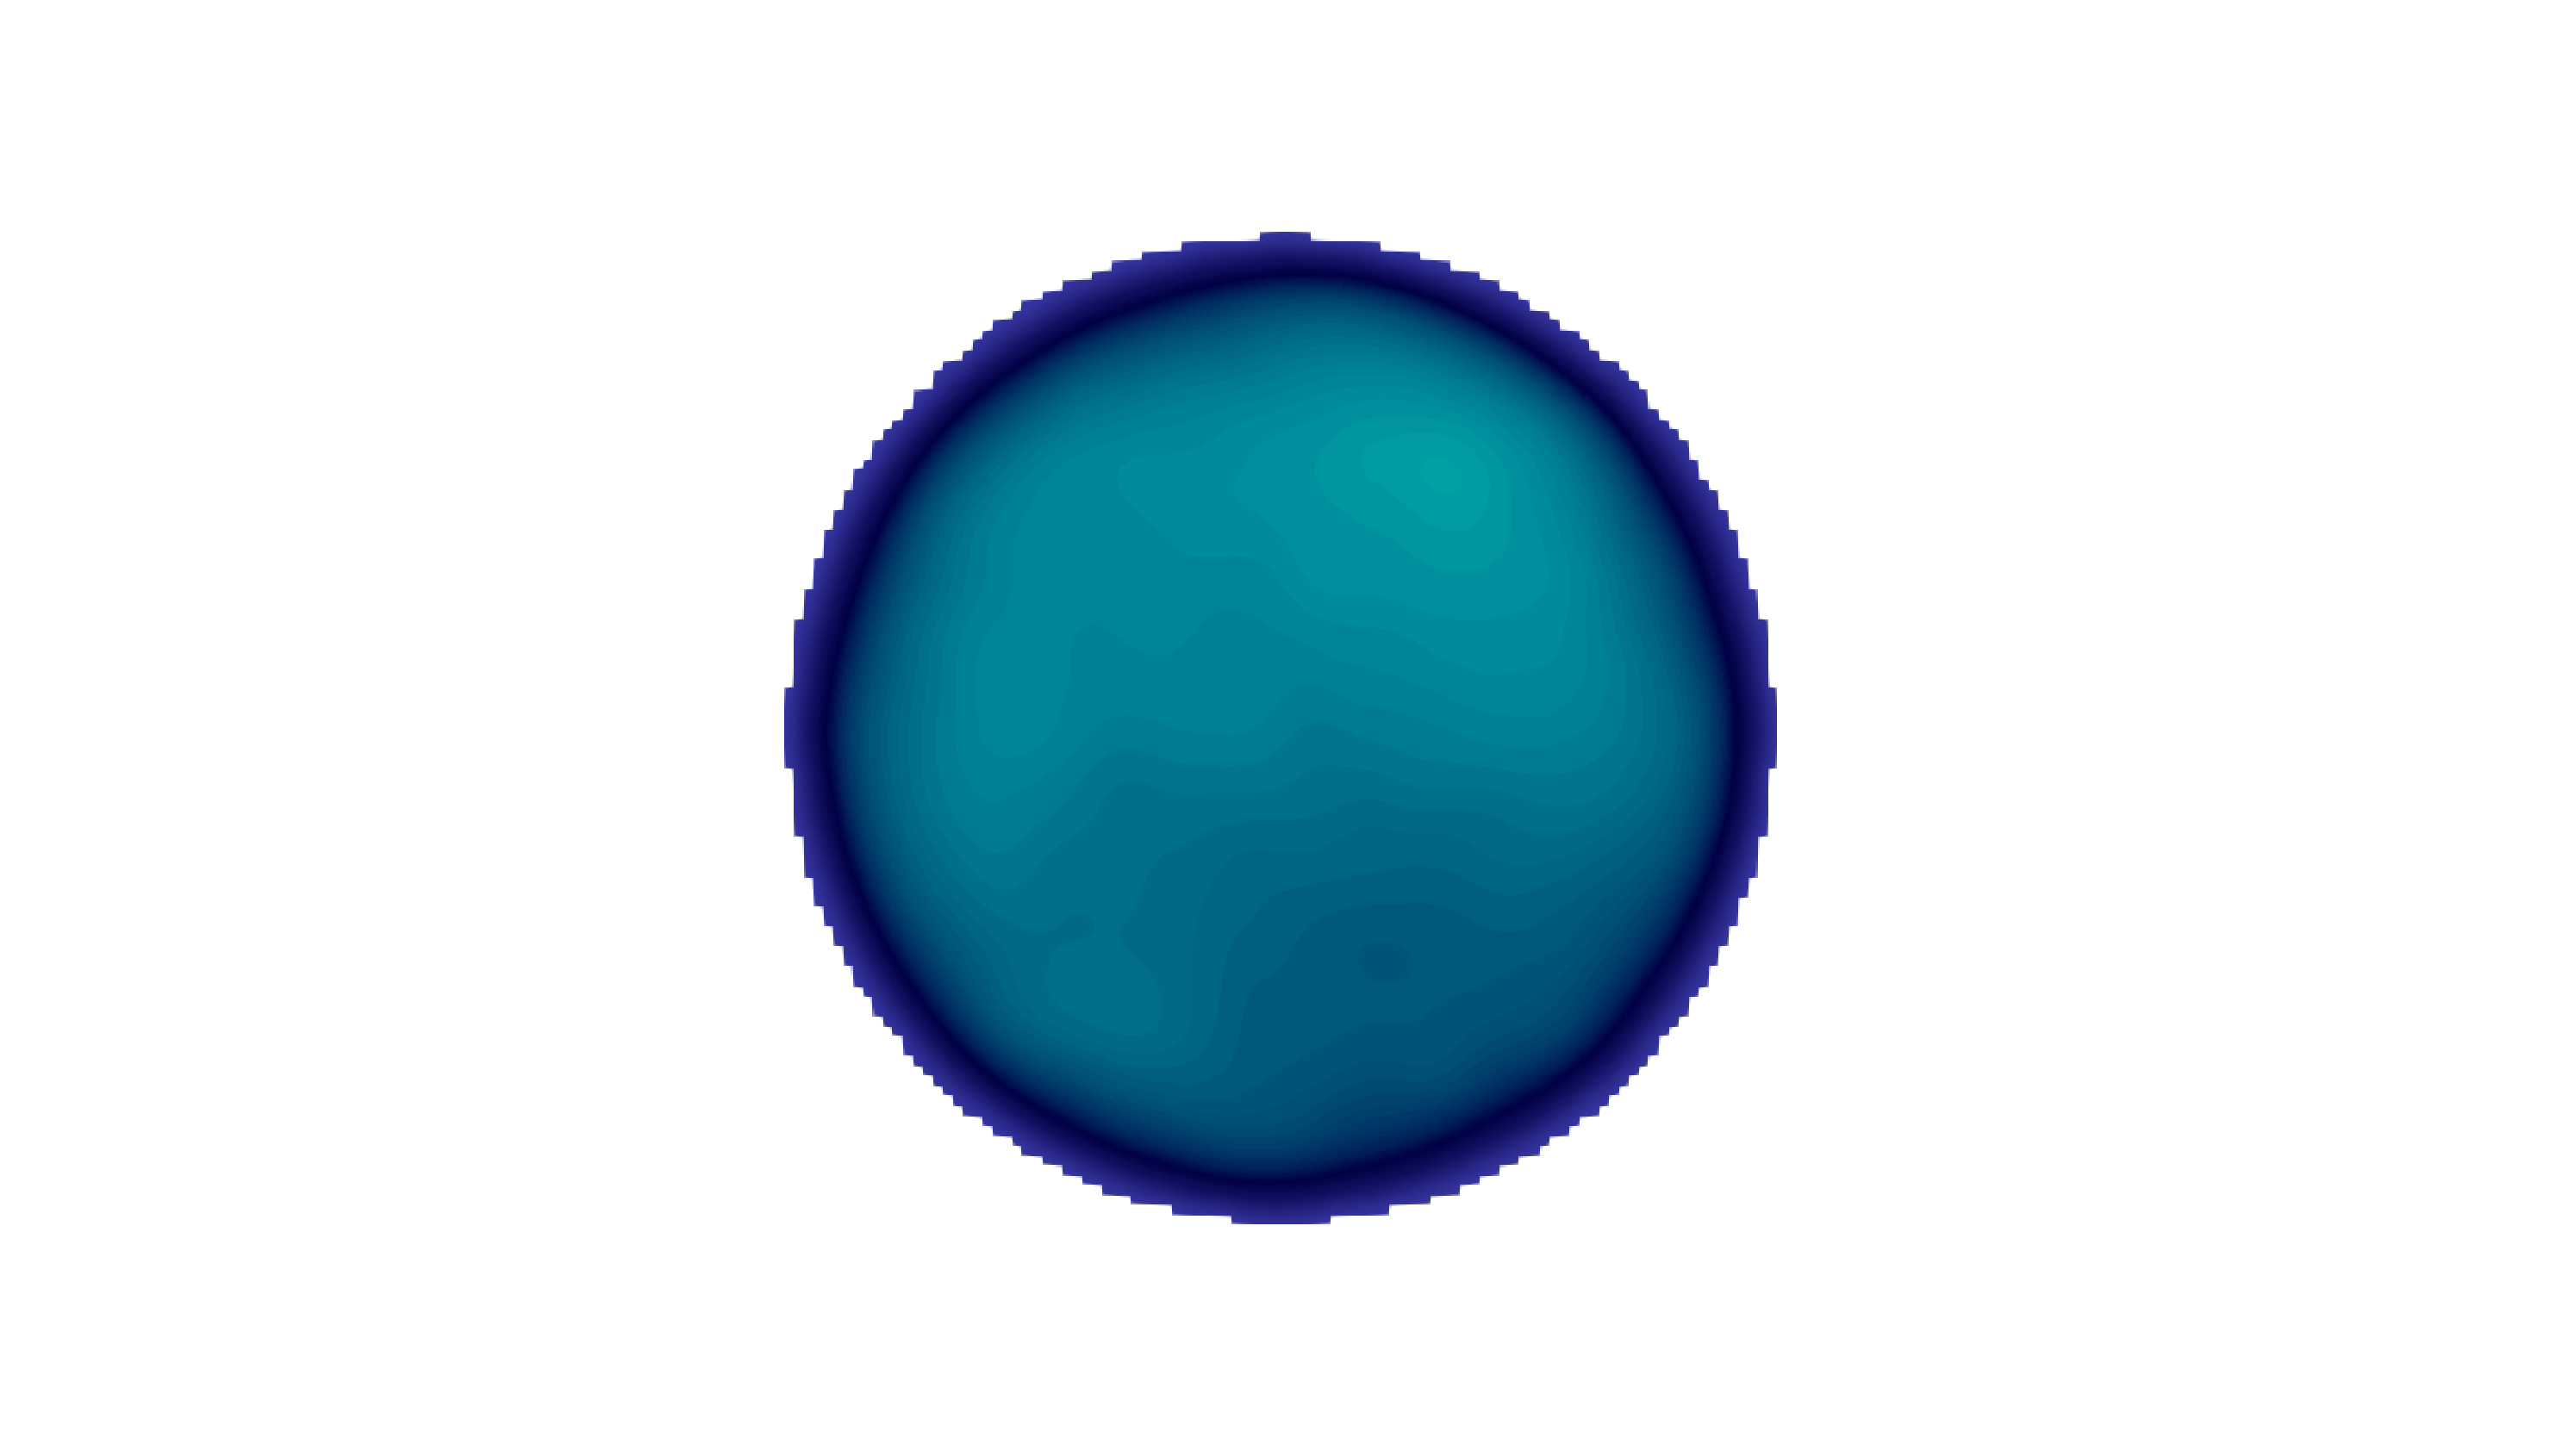
\includegraphics[
		width=0.46\textwidth,
		trim={150mm 20mm 150mm 20mm},
		clip
		]
		{figures/plots/00/00_LPA_mean_veloc.pdf}\hfill
		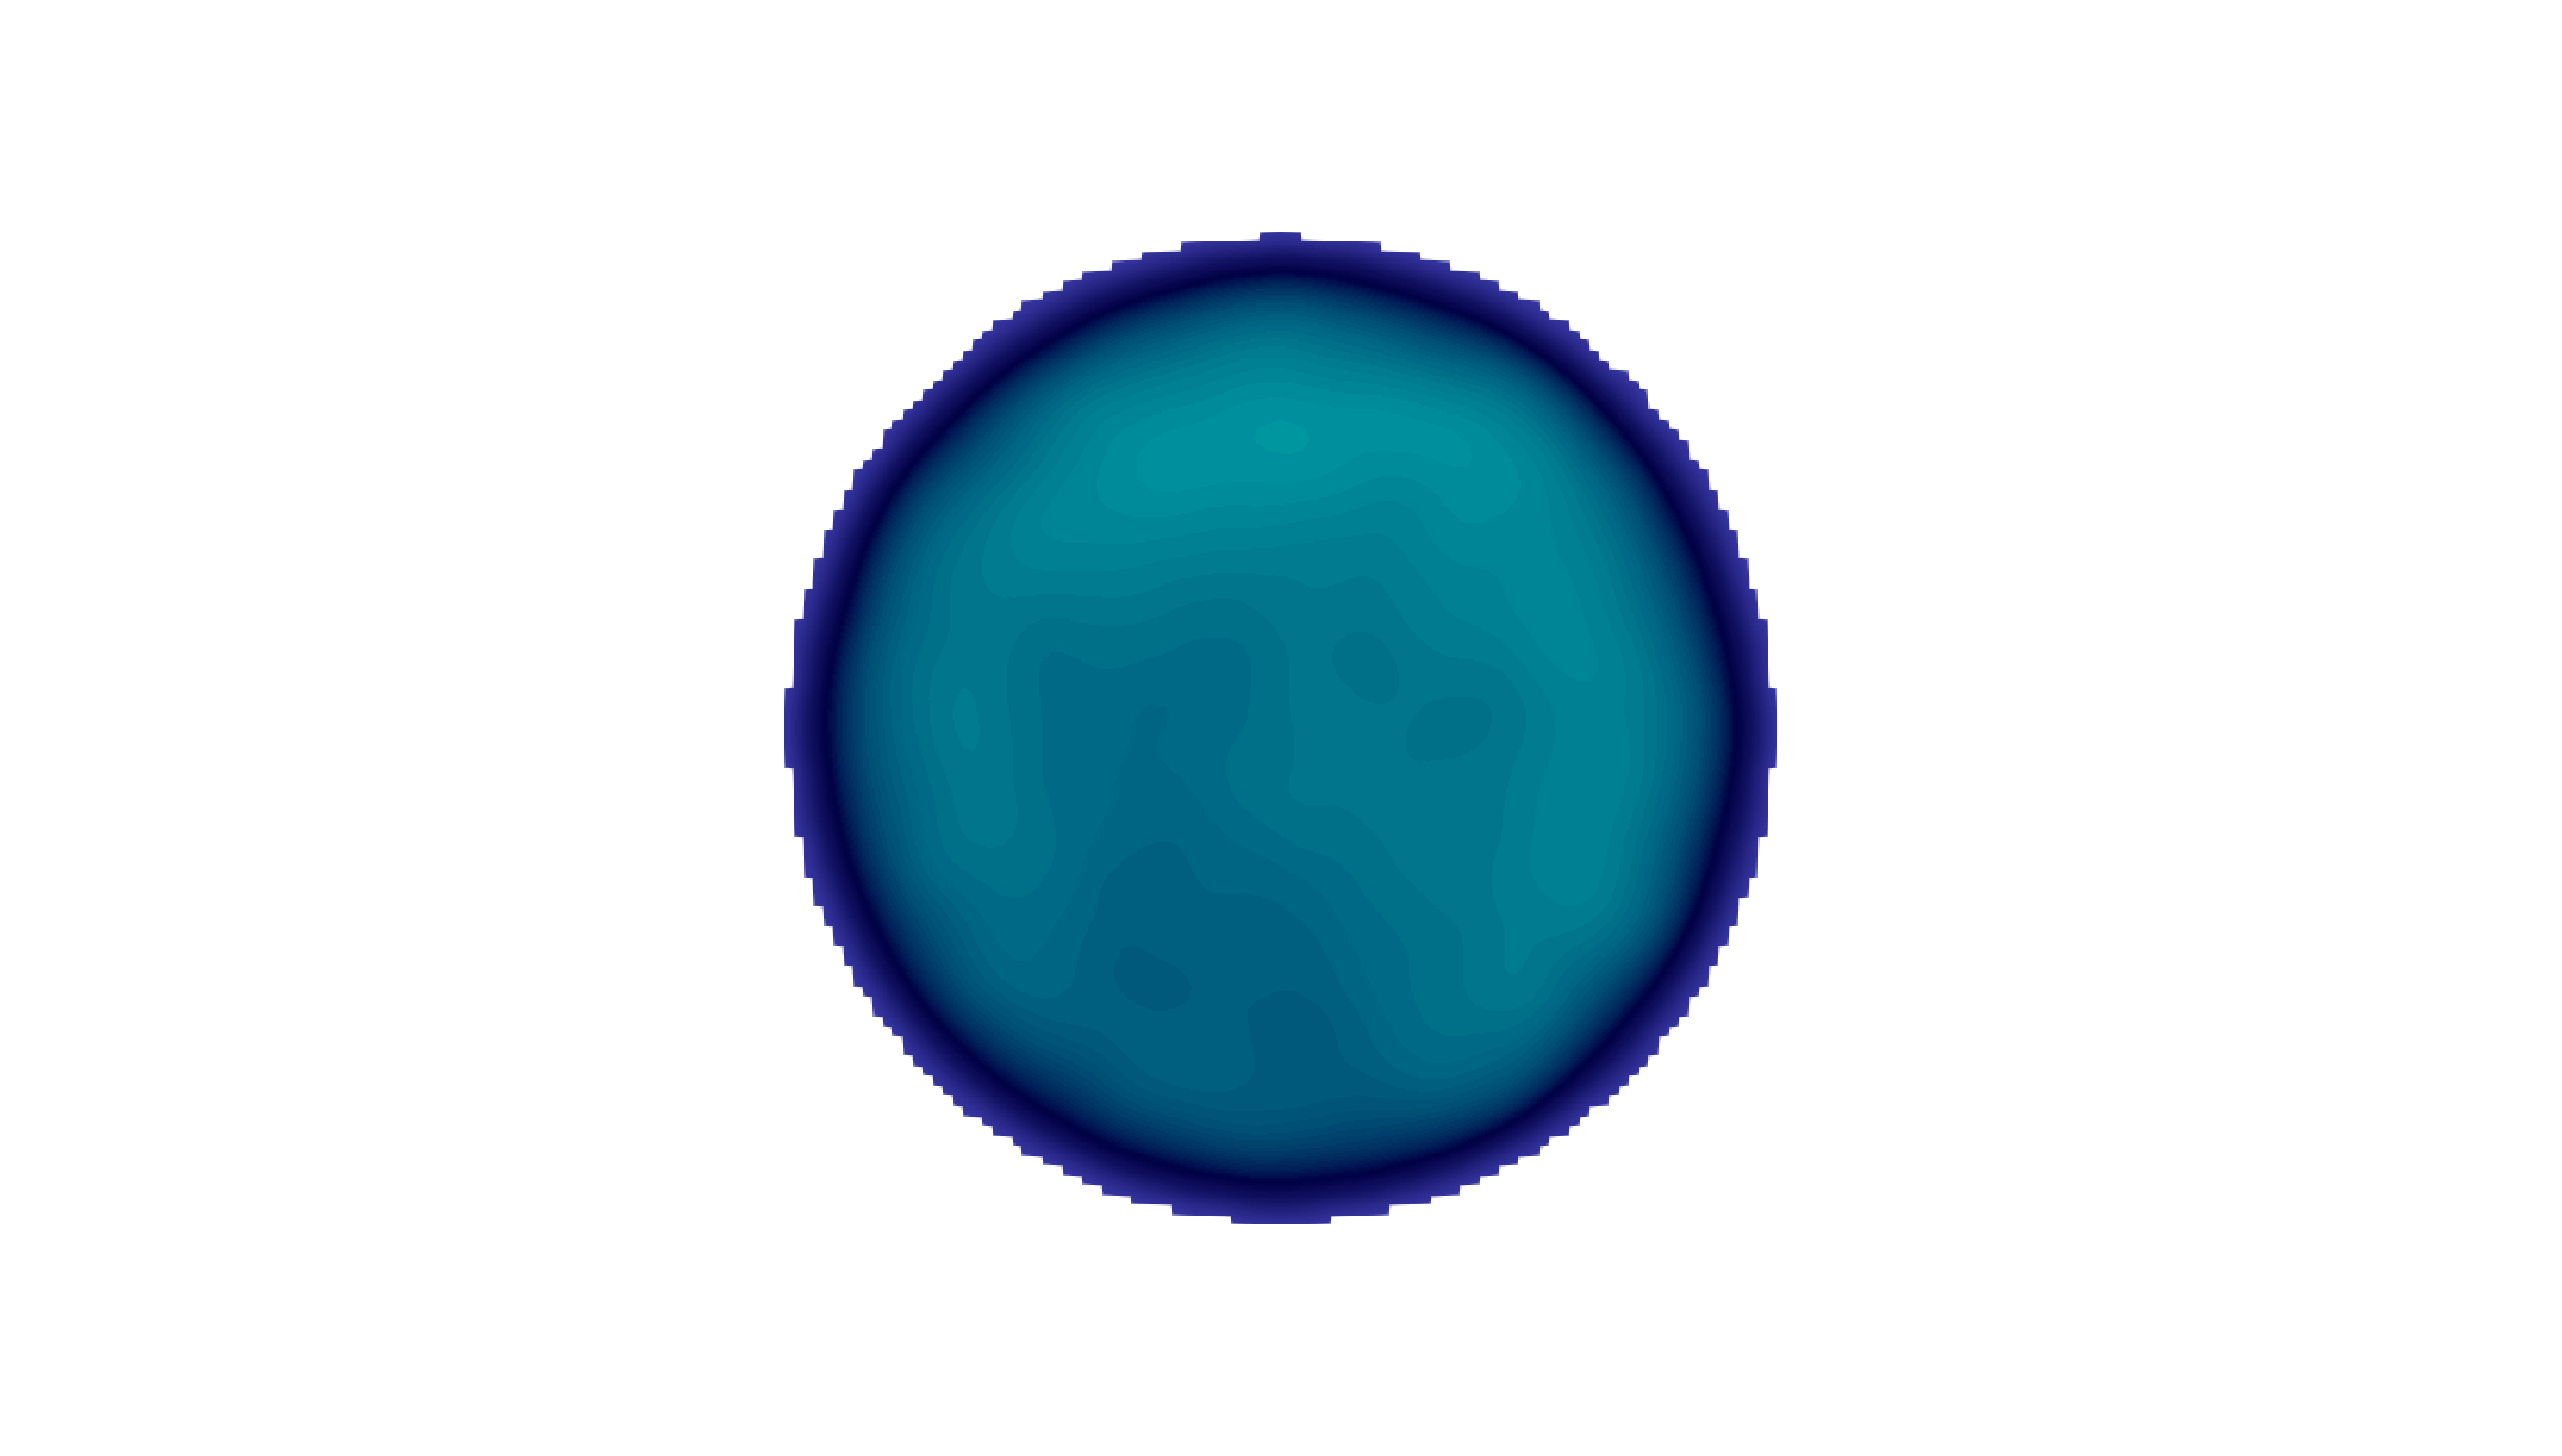
\includegraphics[
		width=0.46\textwidth,
		trim={150mm 20mm 150mm 20mm},
		clip
		]
		{figures/plots/00/00_RPA_mean_veloc.pdf}\\[38pt]
		
		
\includegraphics[
		width=1.08\textwidth,
		]
		{figures/plots/filler.pdf}
		\caption{Magnitudes of mean velocity at the outlets \(\Gamma^{\text{LPA}}_{\text{out}}\) and \(\Gamma^{\text{RPA}}_{\text{out}}\).}
		\label{fig:mean_velocity_outlets00}
	\end{subfigure}
	\begin{center}
		\vspace{-30mm}
		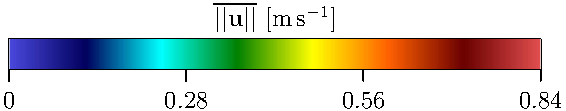
\includegraphics[
		width=0.4\textwidth,
		]
		{figures/plots/mean_veloc_leg.pdf}
		
	\end{center}
	\vspace{14mm}
	
	\begin{subfigure}{0.60\textwidth}
		\centering
		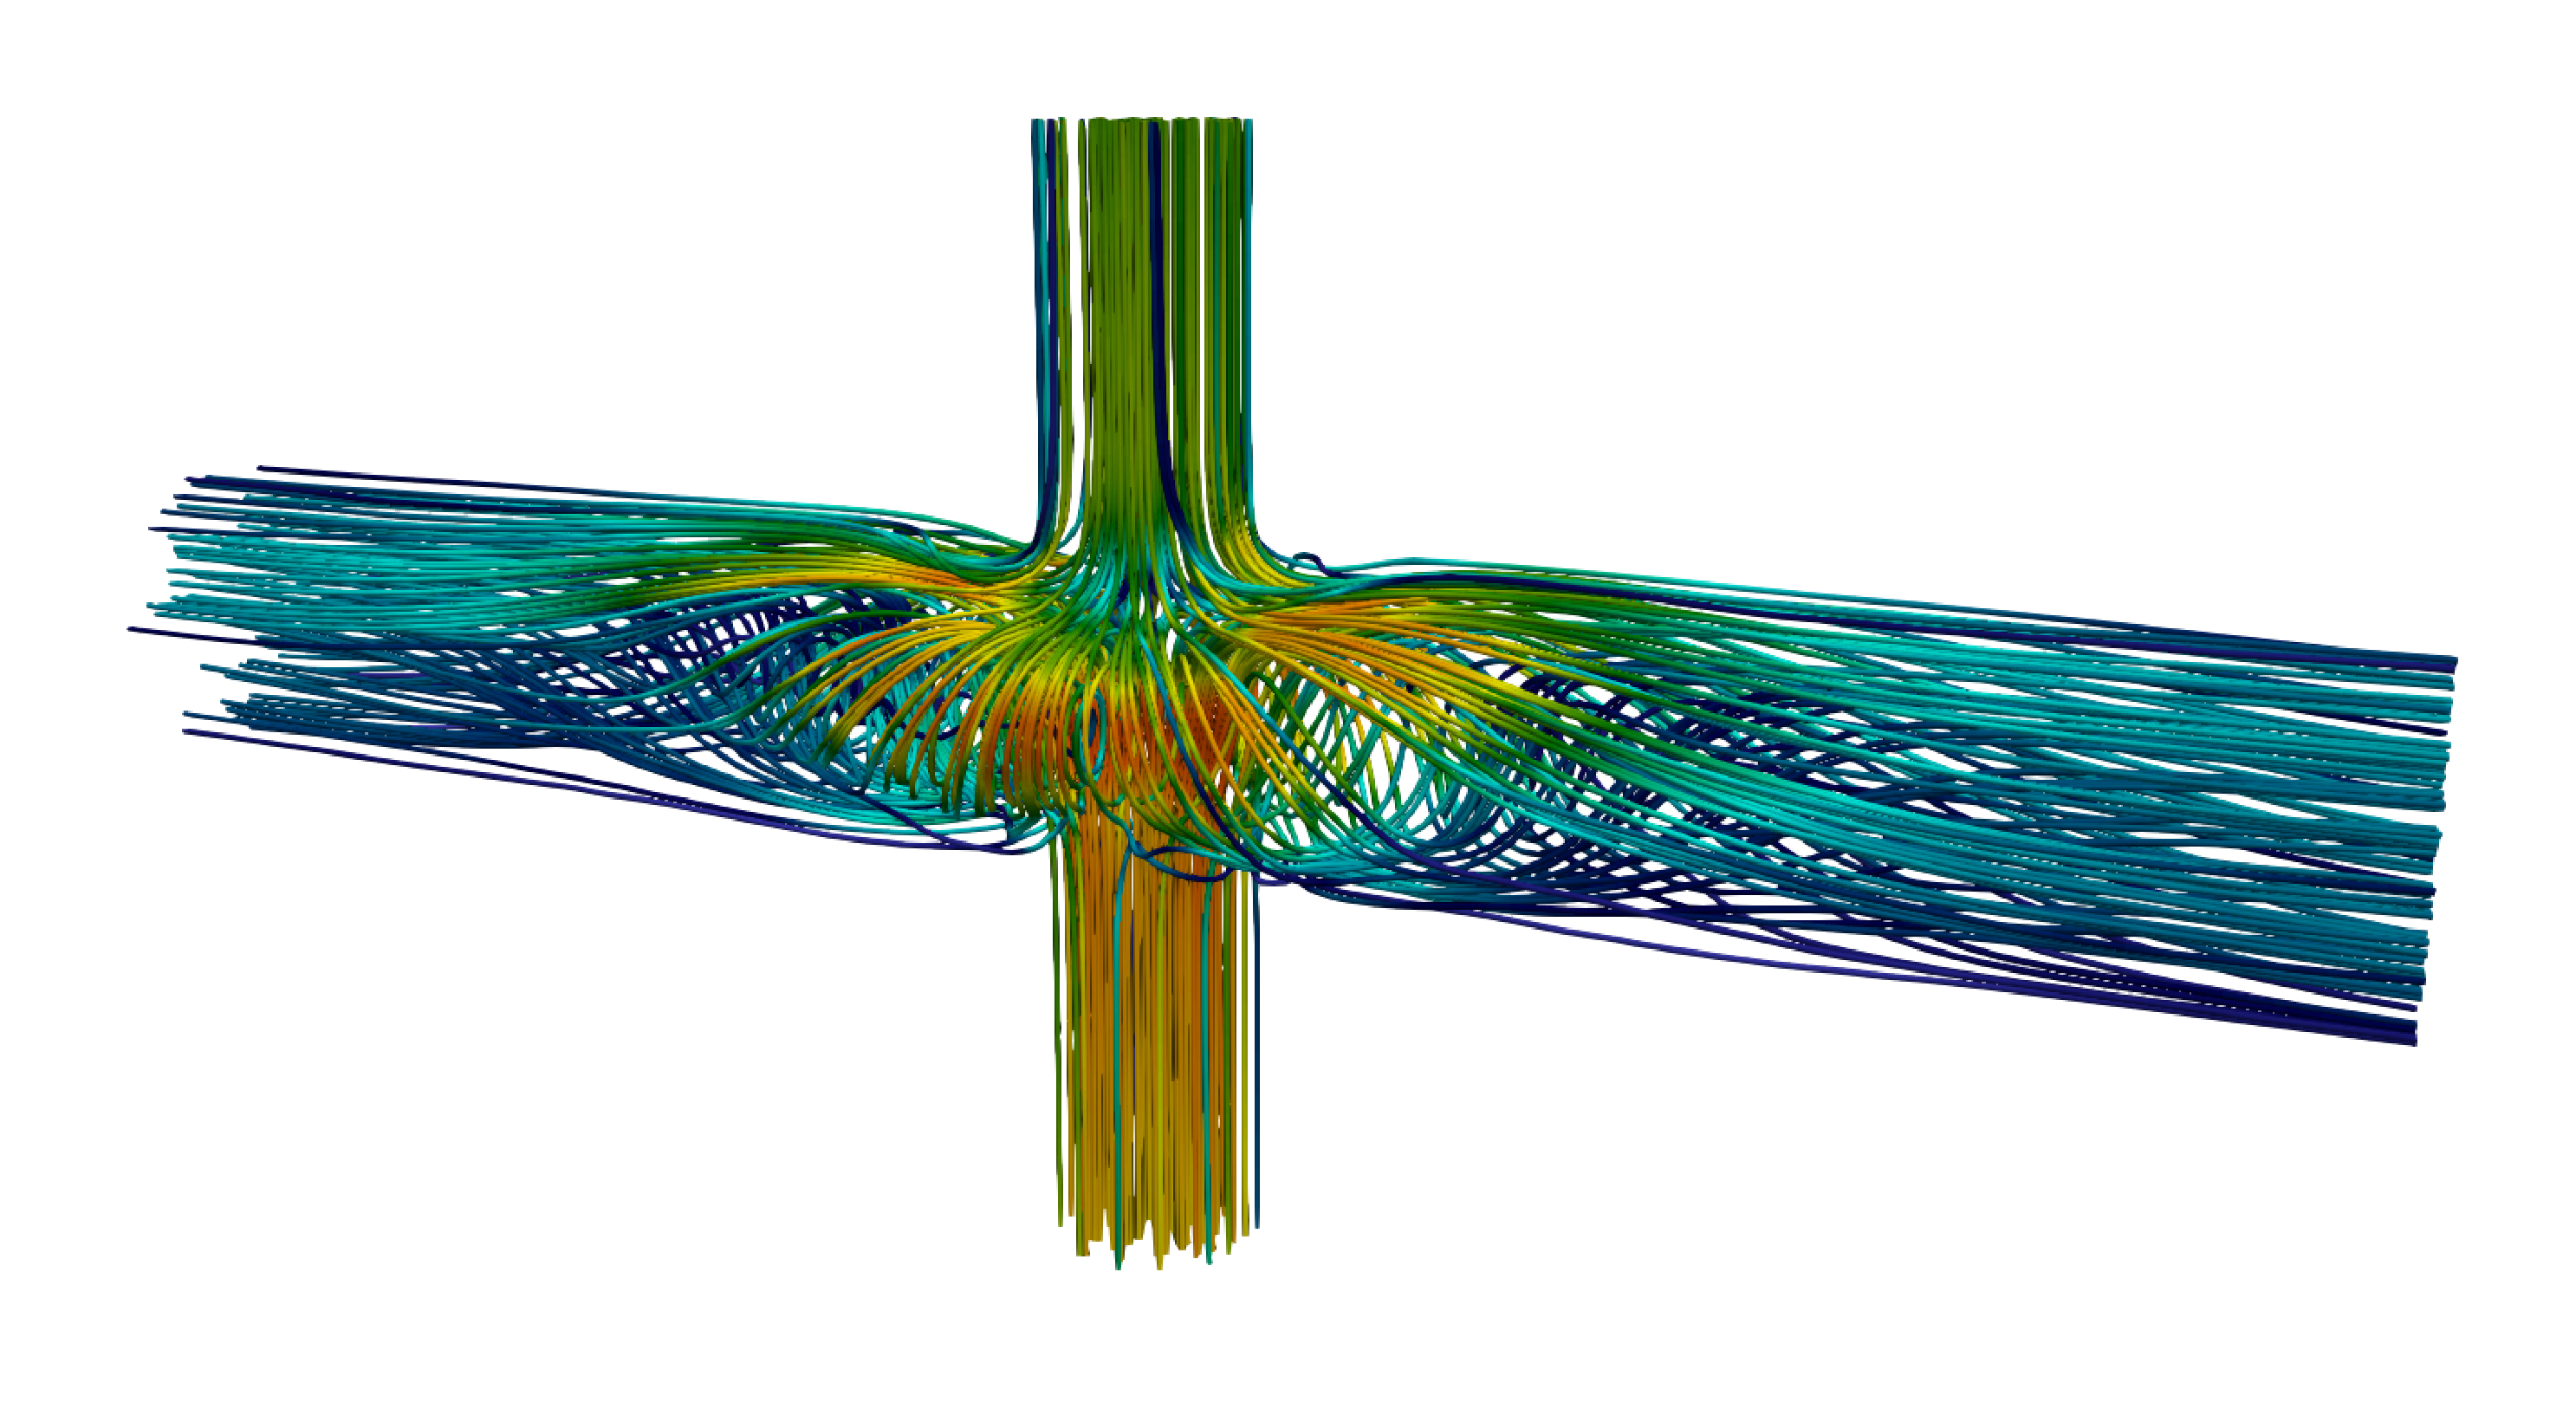
\includegraphics[
		width=\textwidth,
		trim={10mm 10mm 10mm 10mm},
		clip
		]
		{figures/plots/00/00_mean_veloc_streamlines.pdf}%
		\rlap{\hspace{-9cm}\raisebox{0.1cm}{%  move next graphics to top right corner
				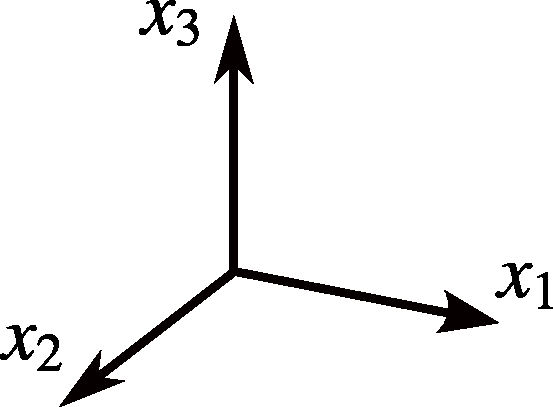
\includegraphics[height=1.5cm]{figures/x1x2x3.pdf}%
		}}
		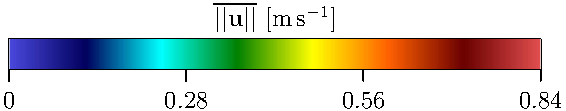
\includegraphics[
		width=0.65\textwidth,
		]
		{figures/plots/mean_veloc_leg.pdf}
		\caption{Streamlines of the mean velocity field illustrating the flow trajectory throughout the geometry.}
		\label{fig:mean_velocity_streamlines00}
	\end{subfigure}\hfill%
	\begin{subfigure}{0.36\textwidth}
		\centering
		\vspace{9mm}
		LPA\hspace{24mm}RPA
		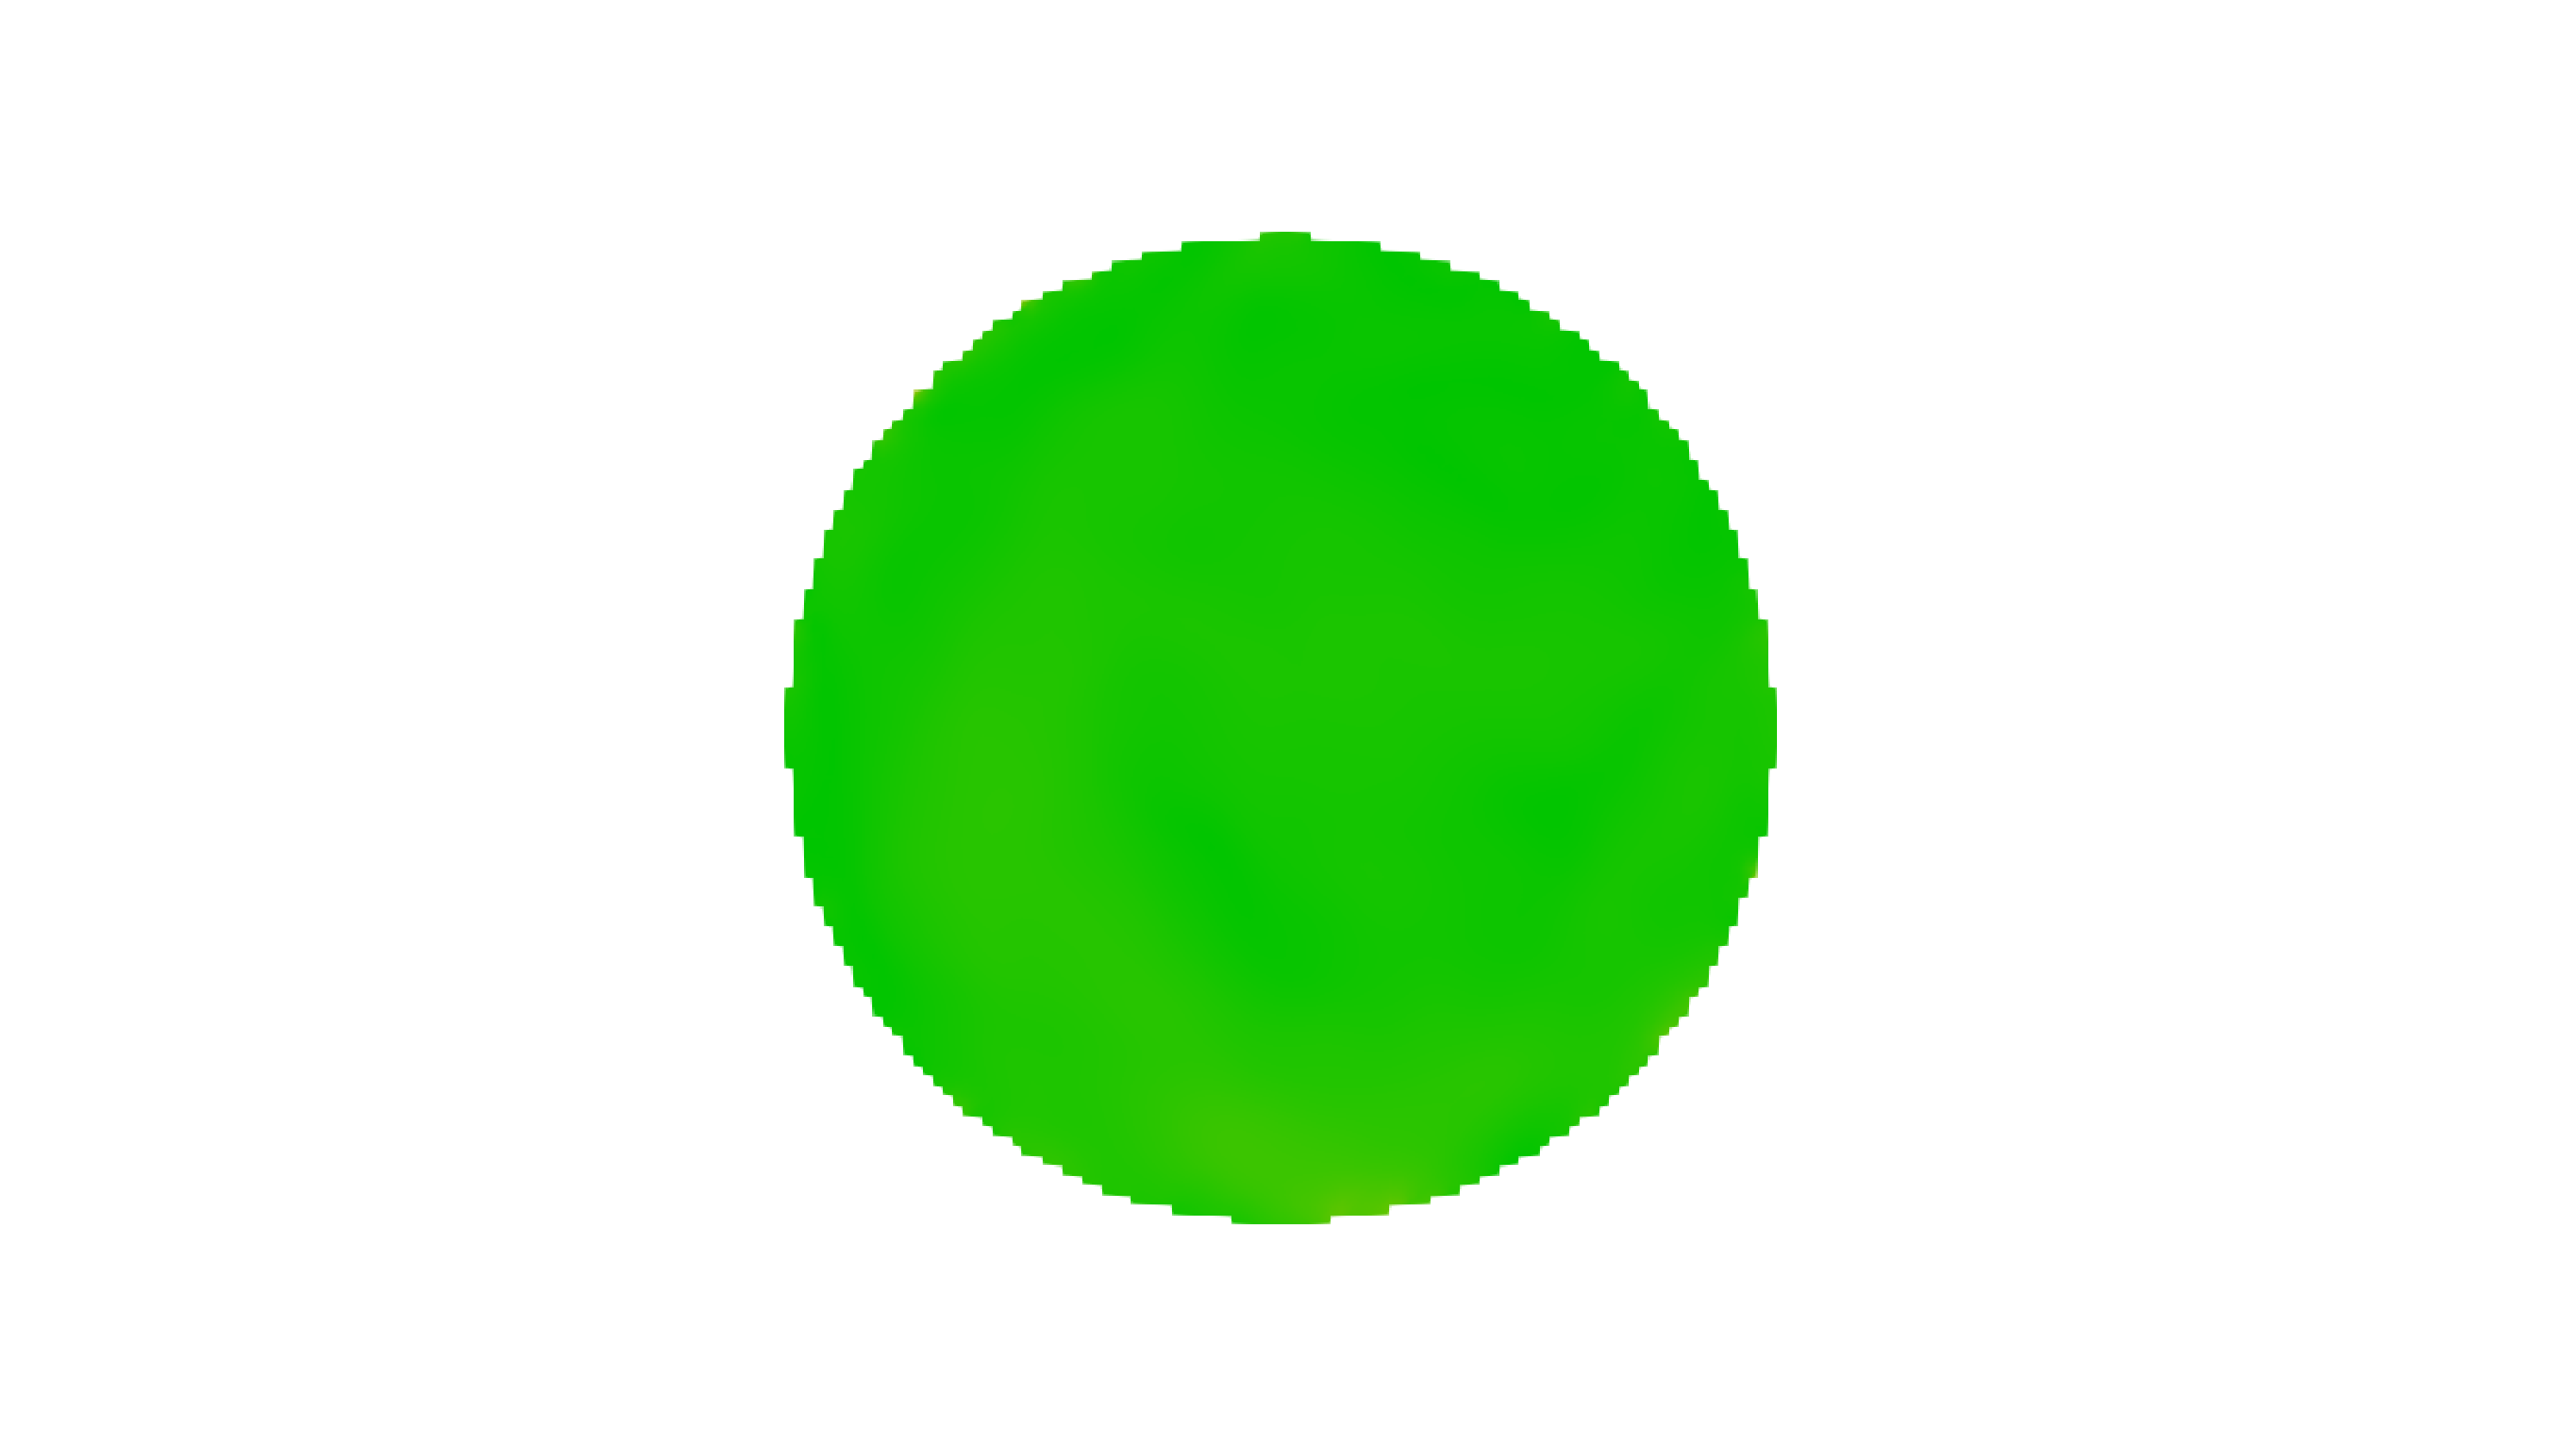
\includegraphics[
		width=0.46\textwidth,
		trim={150mm 20mm 150mm 20mm},
		clip
		]
		{figures/plots/00/00_LPA_angle.pdf}\hfill
		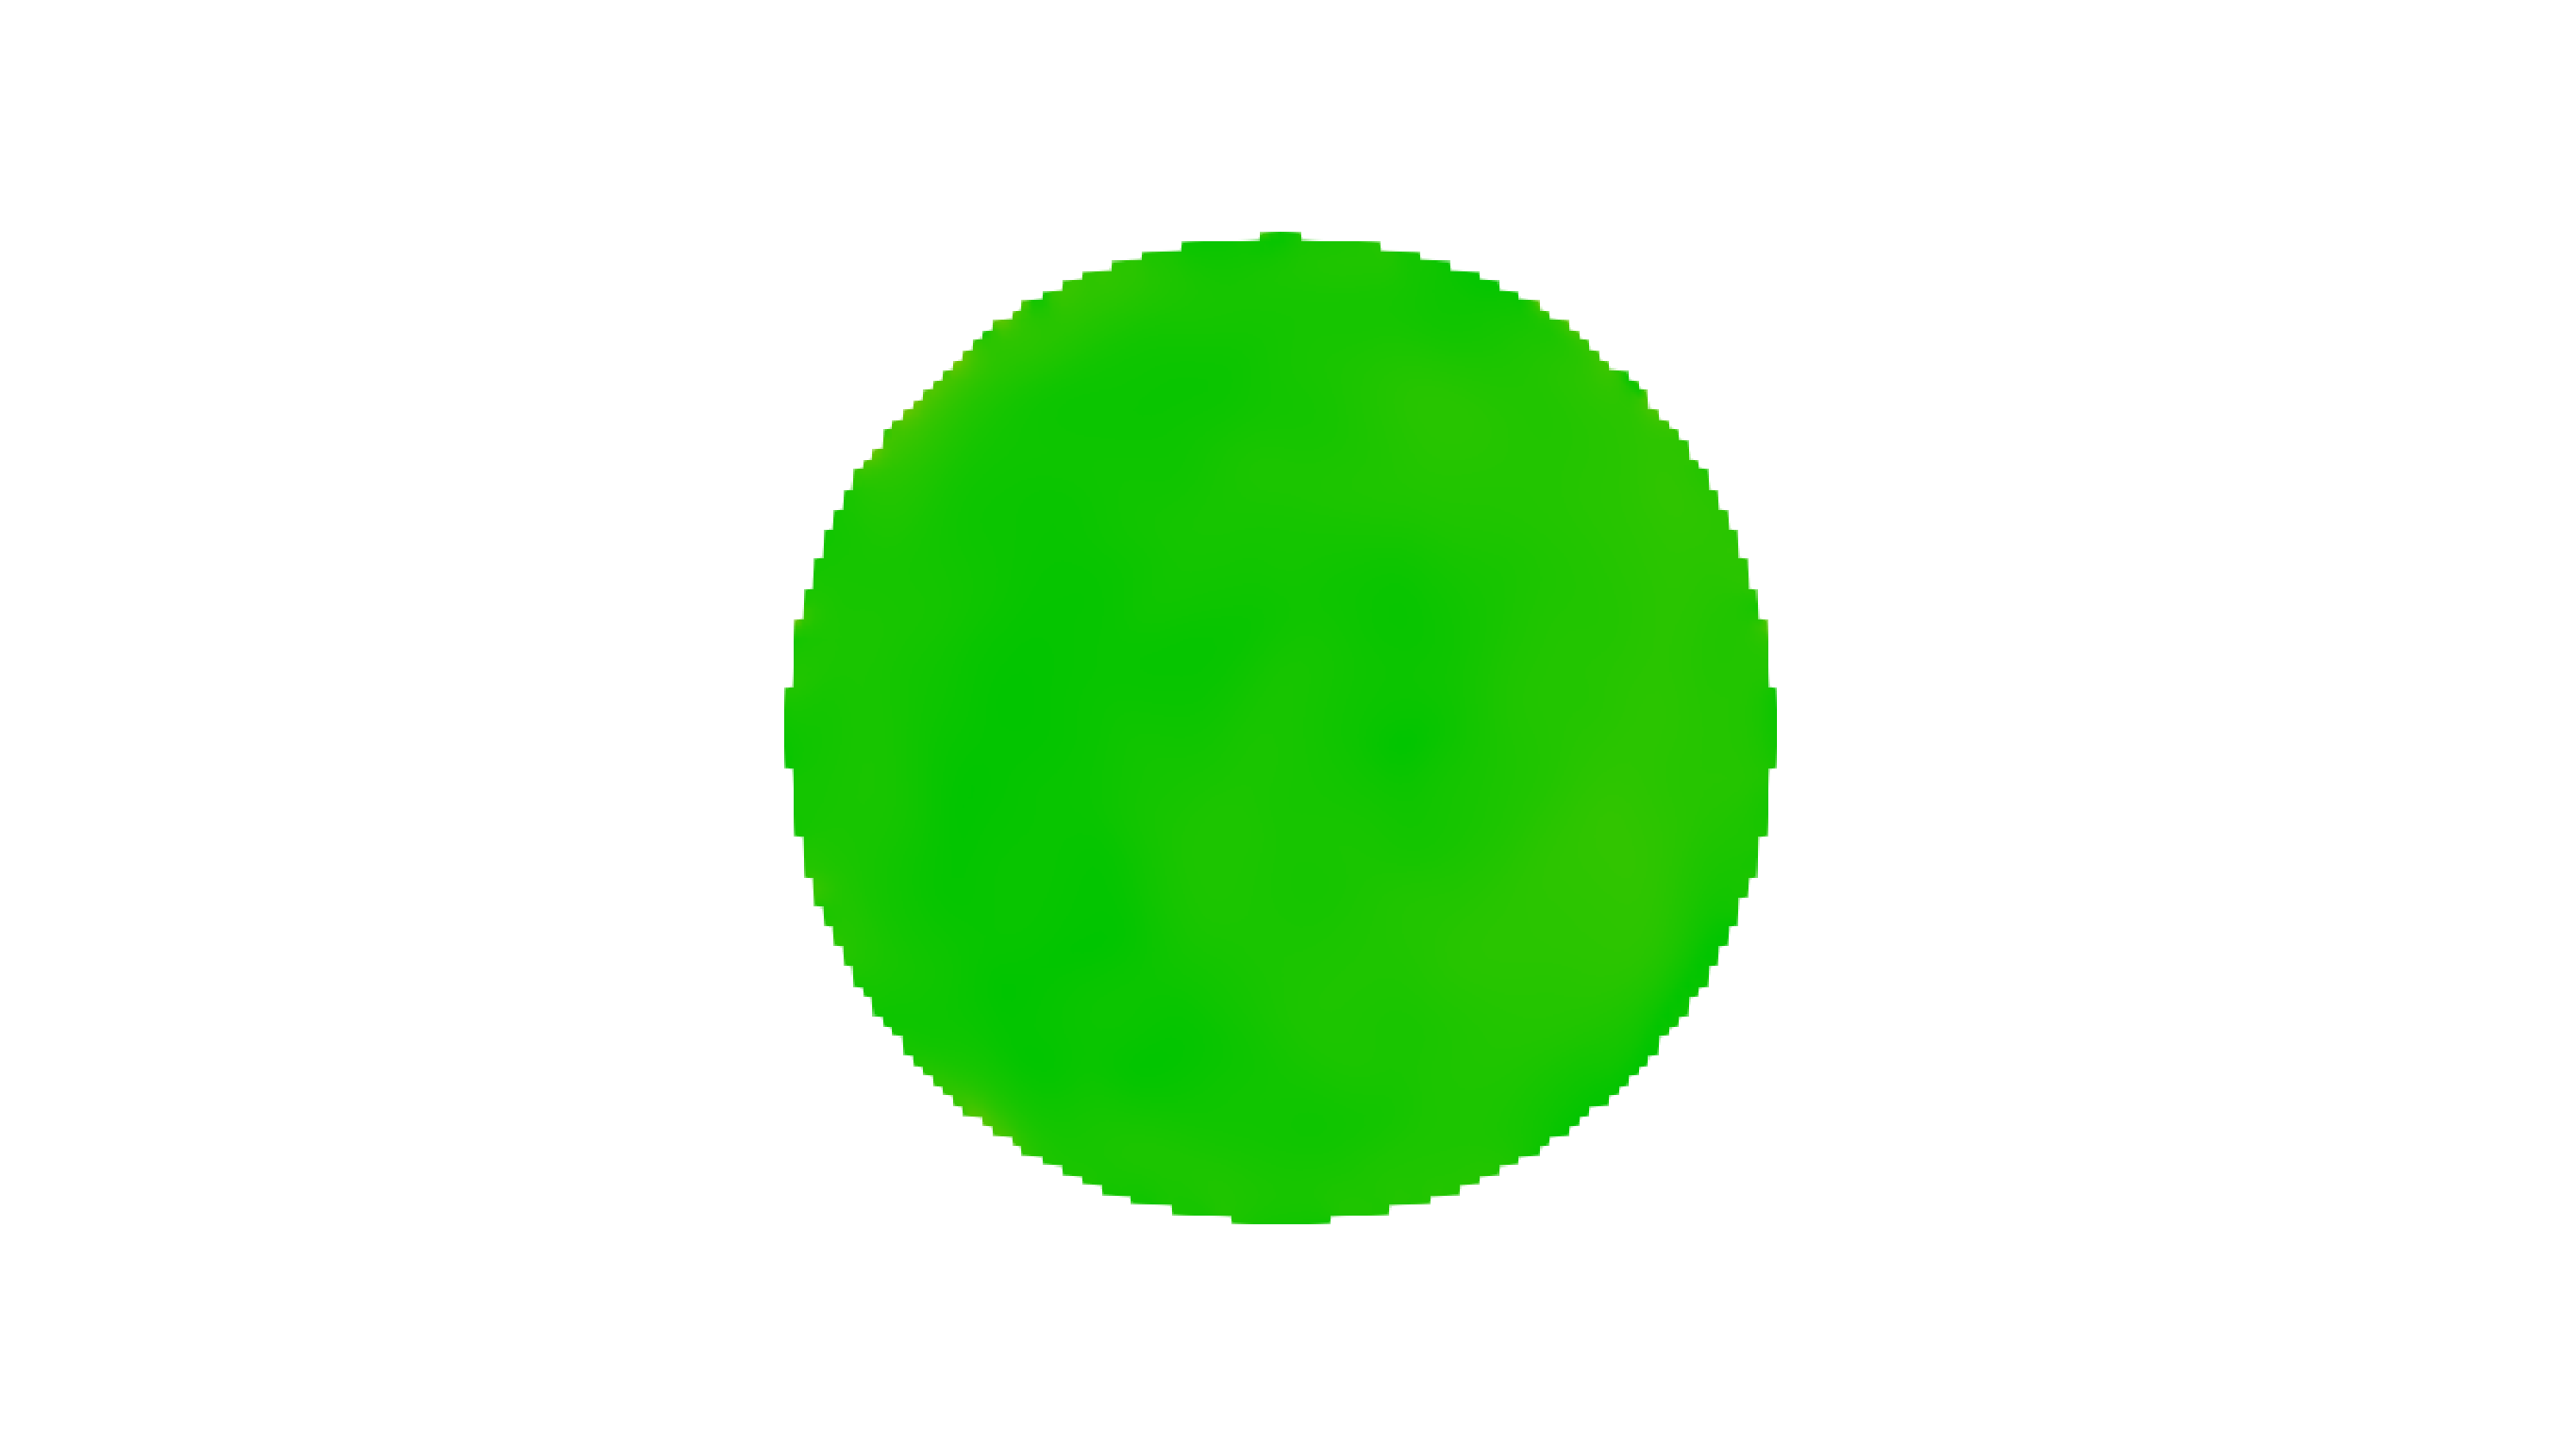
\includegraphics[
		width=0.46\textwidth,
		trim={150mm 20mm 150mm 20mm},
		clip
		]
		{figures/plots/00/00_RPA_angle.pdf}
		
		
\includegraphics[
		width=0.99\textwidth,
		]
		{figures/plots/filler.pdf}
		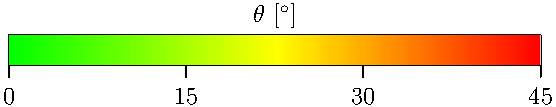
\includegraphics[
		width=1.05\textwidth,
		]
		{figures/plots/angle_leg.pdf}
		\caption{Angle between the mean velocity vector and the normal direction at the outlets \(\Gamma^{\text{LPA}}_{\text{out}}\) and \(\Gamma^{\text{RPA}}_{\text{out}}\).}
		\label{fig:velocity_angle_outlets00}
	\end{subfigure}
	
	\vspace{2mm}
	\caption{Overview of mean velocity fields and outlet characteristics for the case of point P$_0$, i.e., when $o_1 = 0{,}0 \, \mathrm{cm}$. Subfigure (a) shows the velocity magnitude field, (b) displays outlet-specific velocity magnitudes, (c) presents streamlines of the mean velocity field, and (d) details the angular alignment of velocity vectors with outlet normals.}
	\label{fig:mean_velocity_analysis00}
\end{figure}

\newgeometry{top=1.7cm}

\begin{figure}[H]
	\subsection*{Shear rate}
	\vspace{-3mm}
	\rule{\textwidth}{0.4pt}\\
	\begin{subfigure}{0.48\textwidth}
		%		\vspace{-8mm}
		\centering
		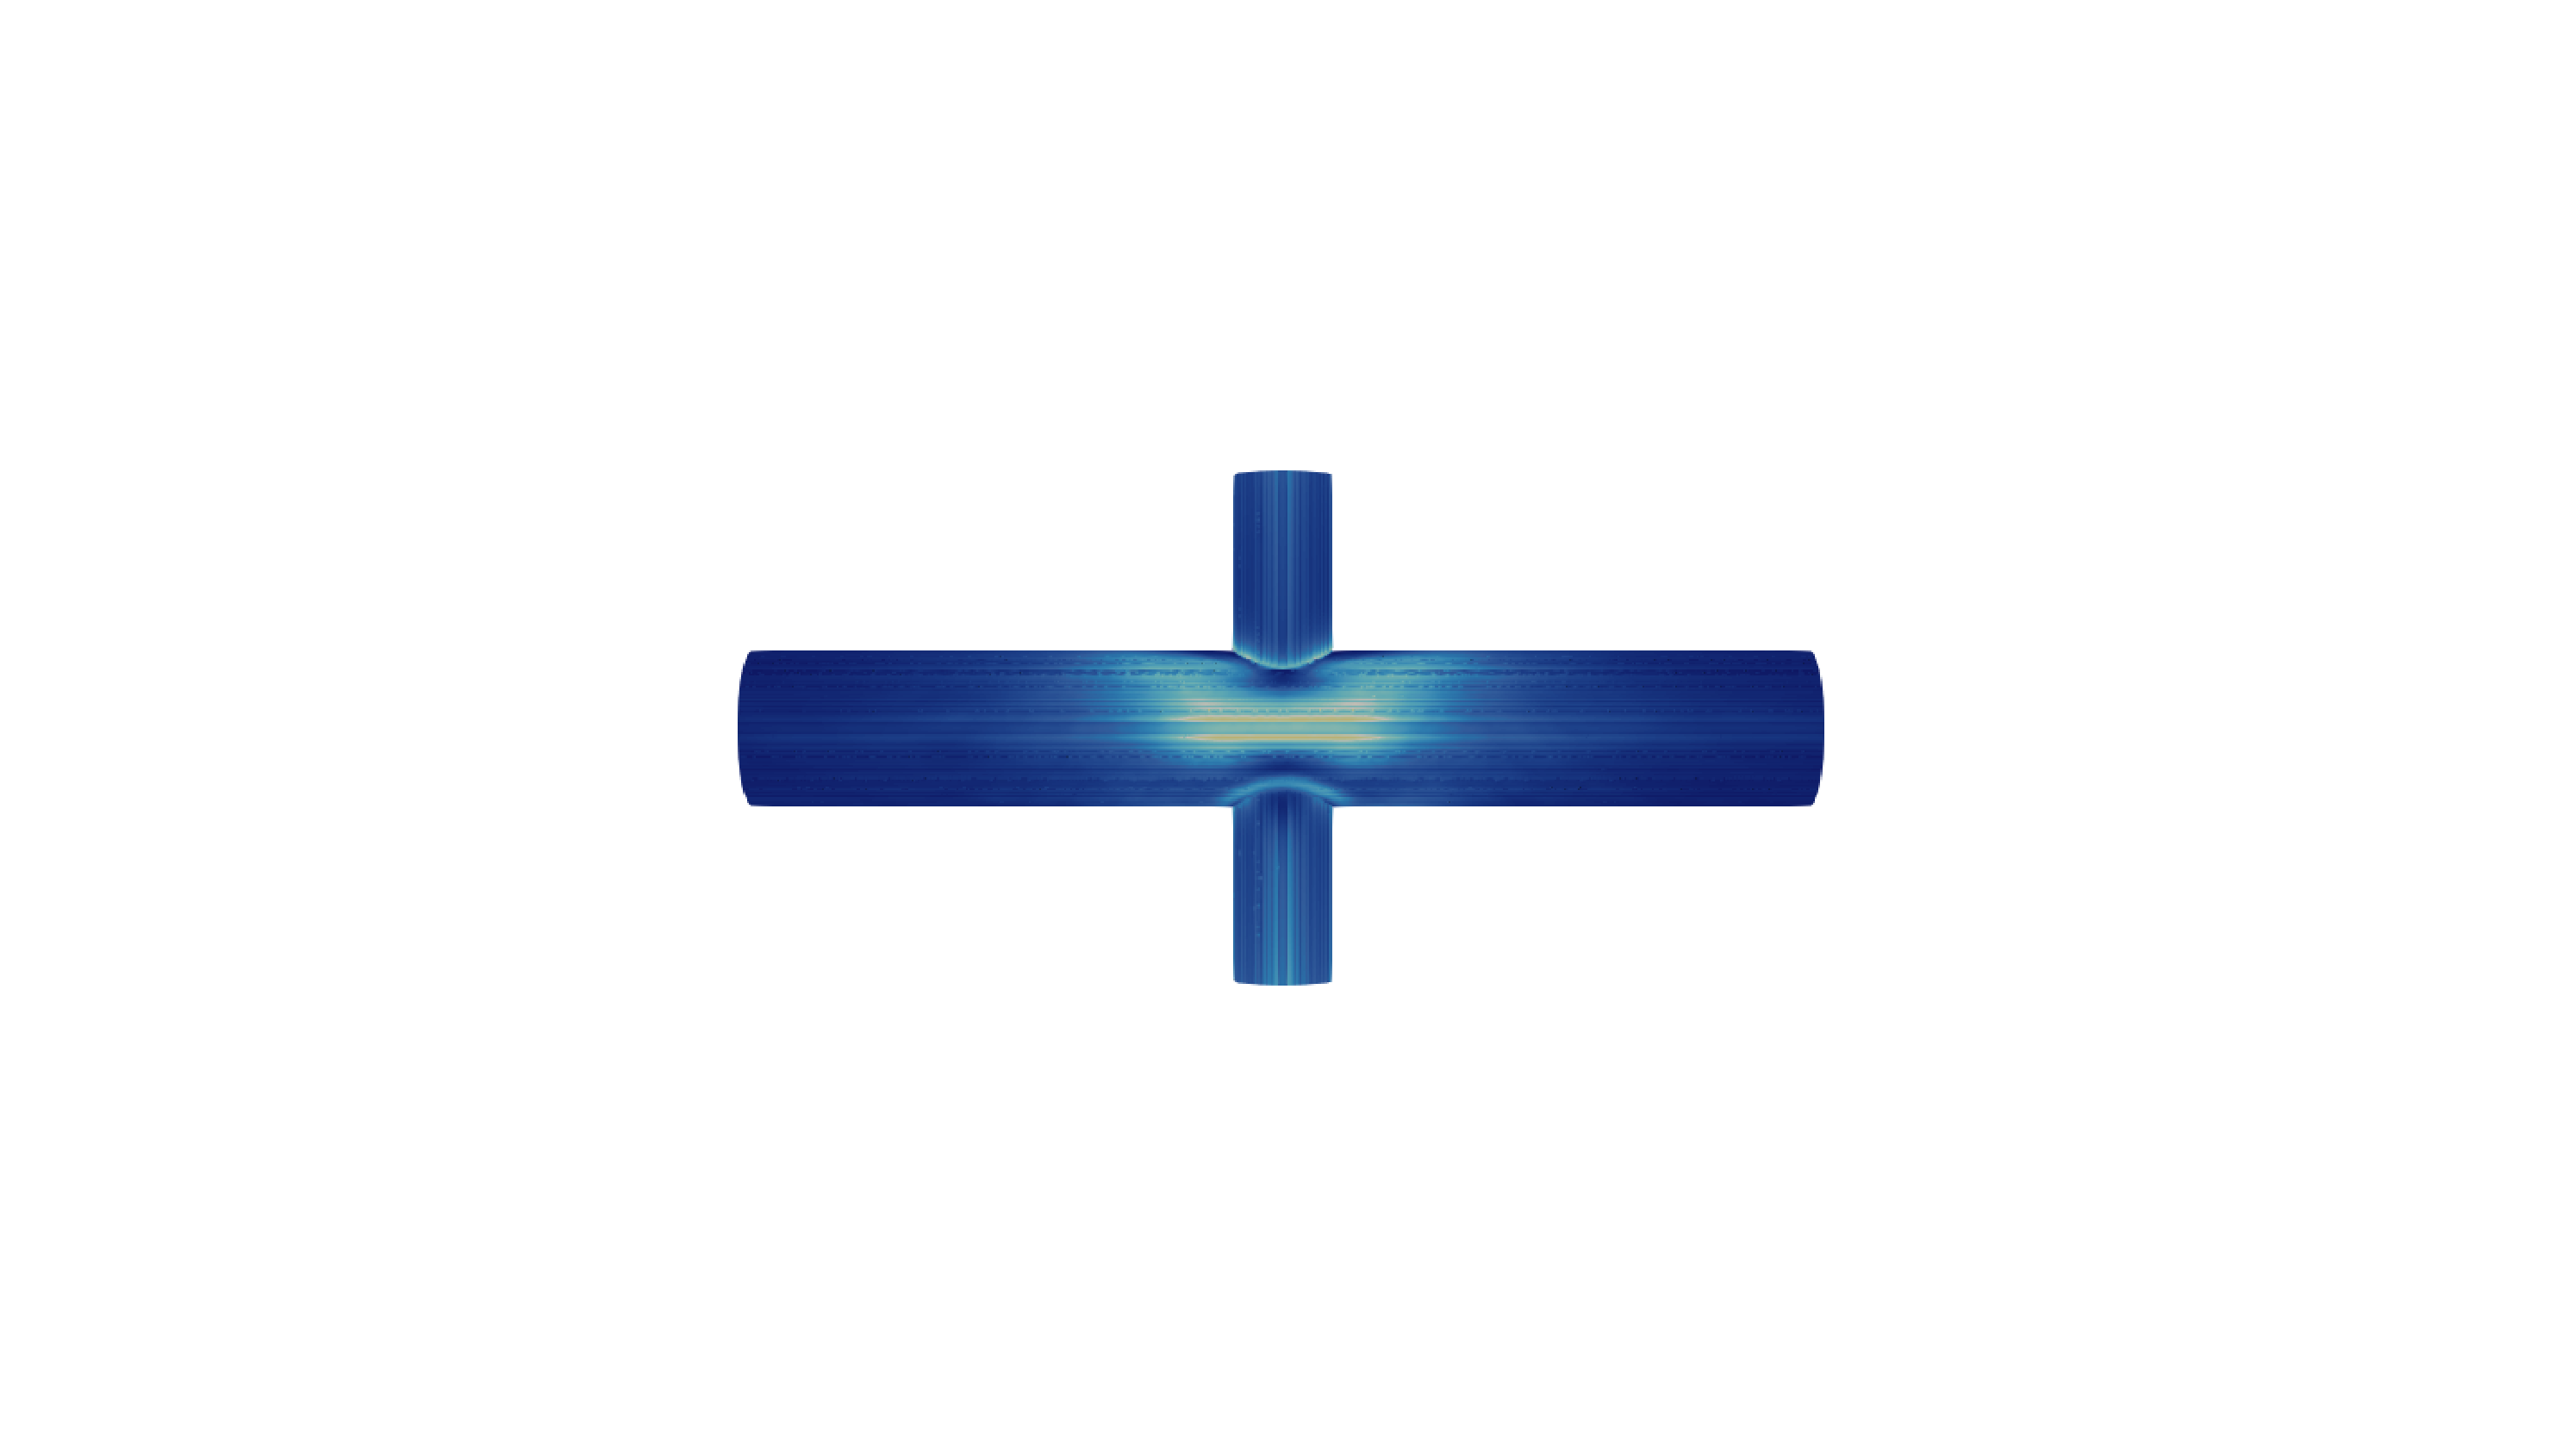
\includegraphics[
		width=\textwidth,
		trim={130mm 85mm 130mm 80mm},
		clip
		]
		{figures/plots/00/00_mean_stress_xz.pdf}%
		\rlap{\hspace{-7cm}\raisebox{-0.5cm}{%  move next graphics to top right corner
				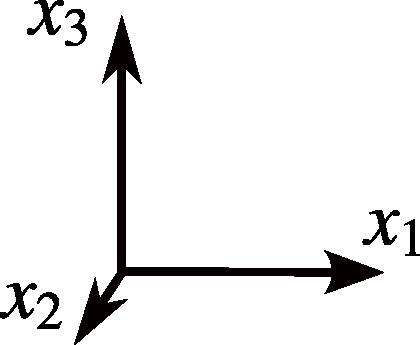
\includegraphics[height=1.5cm]{figures/x1x2x3-side.pdf}%
		}}
		
		
		
\includegraphics[
		width=0.85\textwidth,
		]
		{figures/plots/filler.pdf}
		\caption{Mean shear rate in the \(x_1\)-\(x_3\) plane.}
		\label{fig:mean_stress_xz00}
		
	\end{subfigure}\hfill%
	\begin{subfigure}{0.48\textwidth}
		%		\vspace{-8mm}
		\centering
		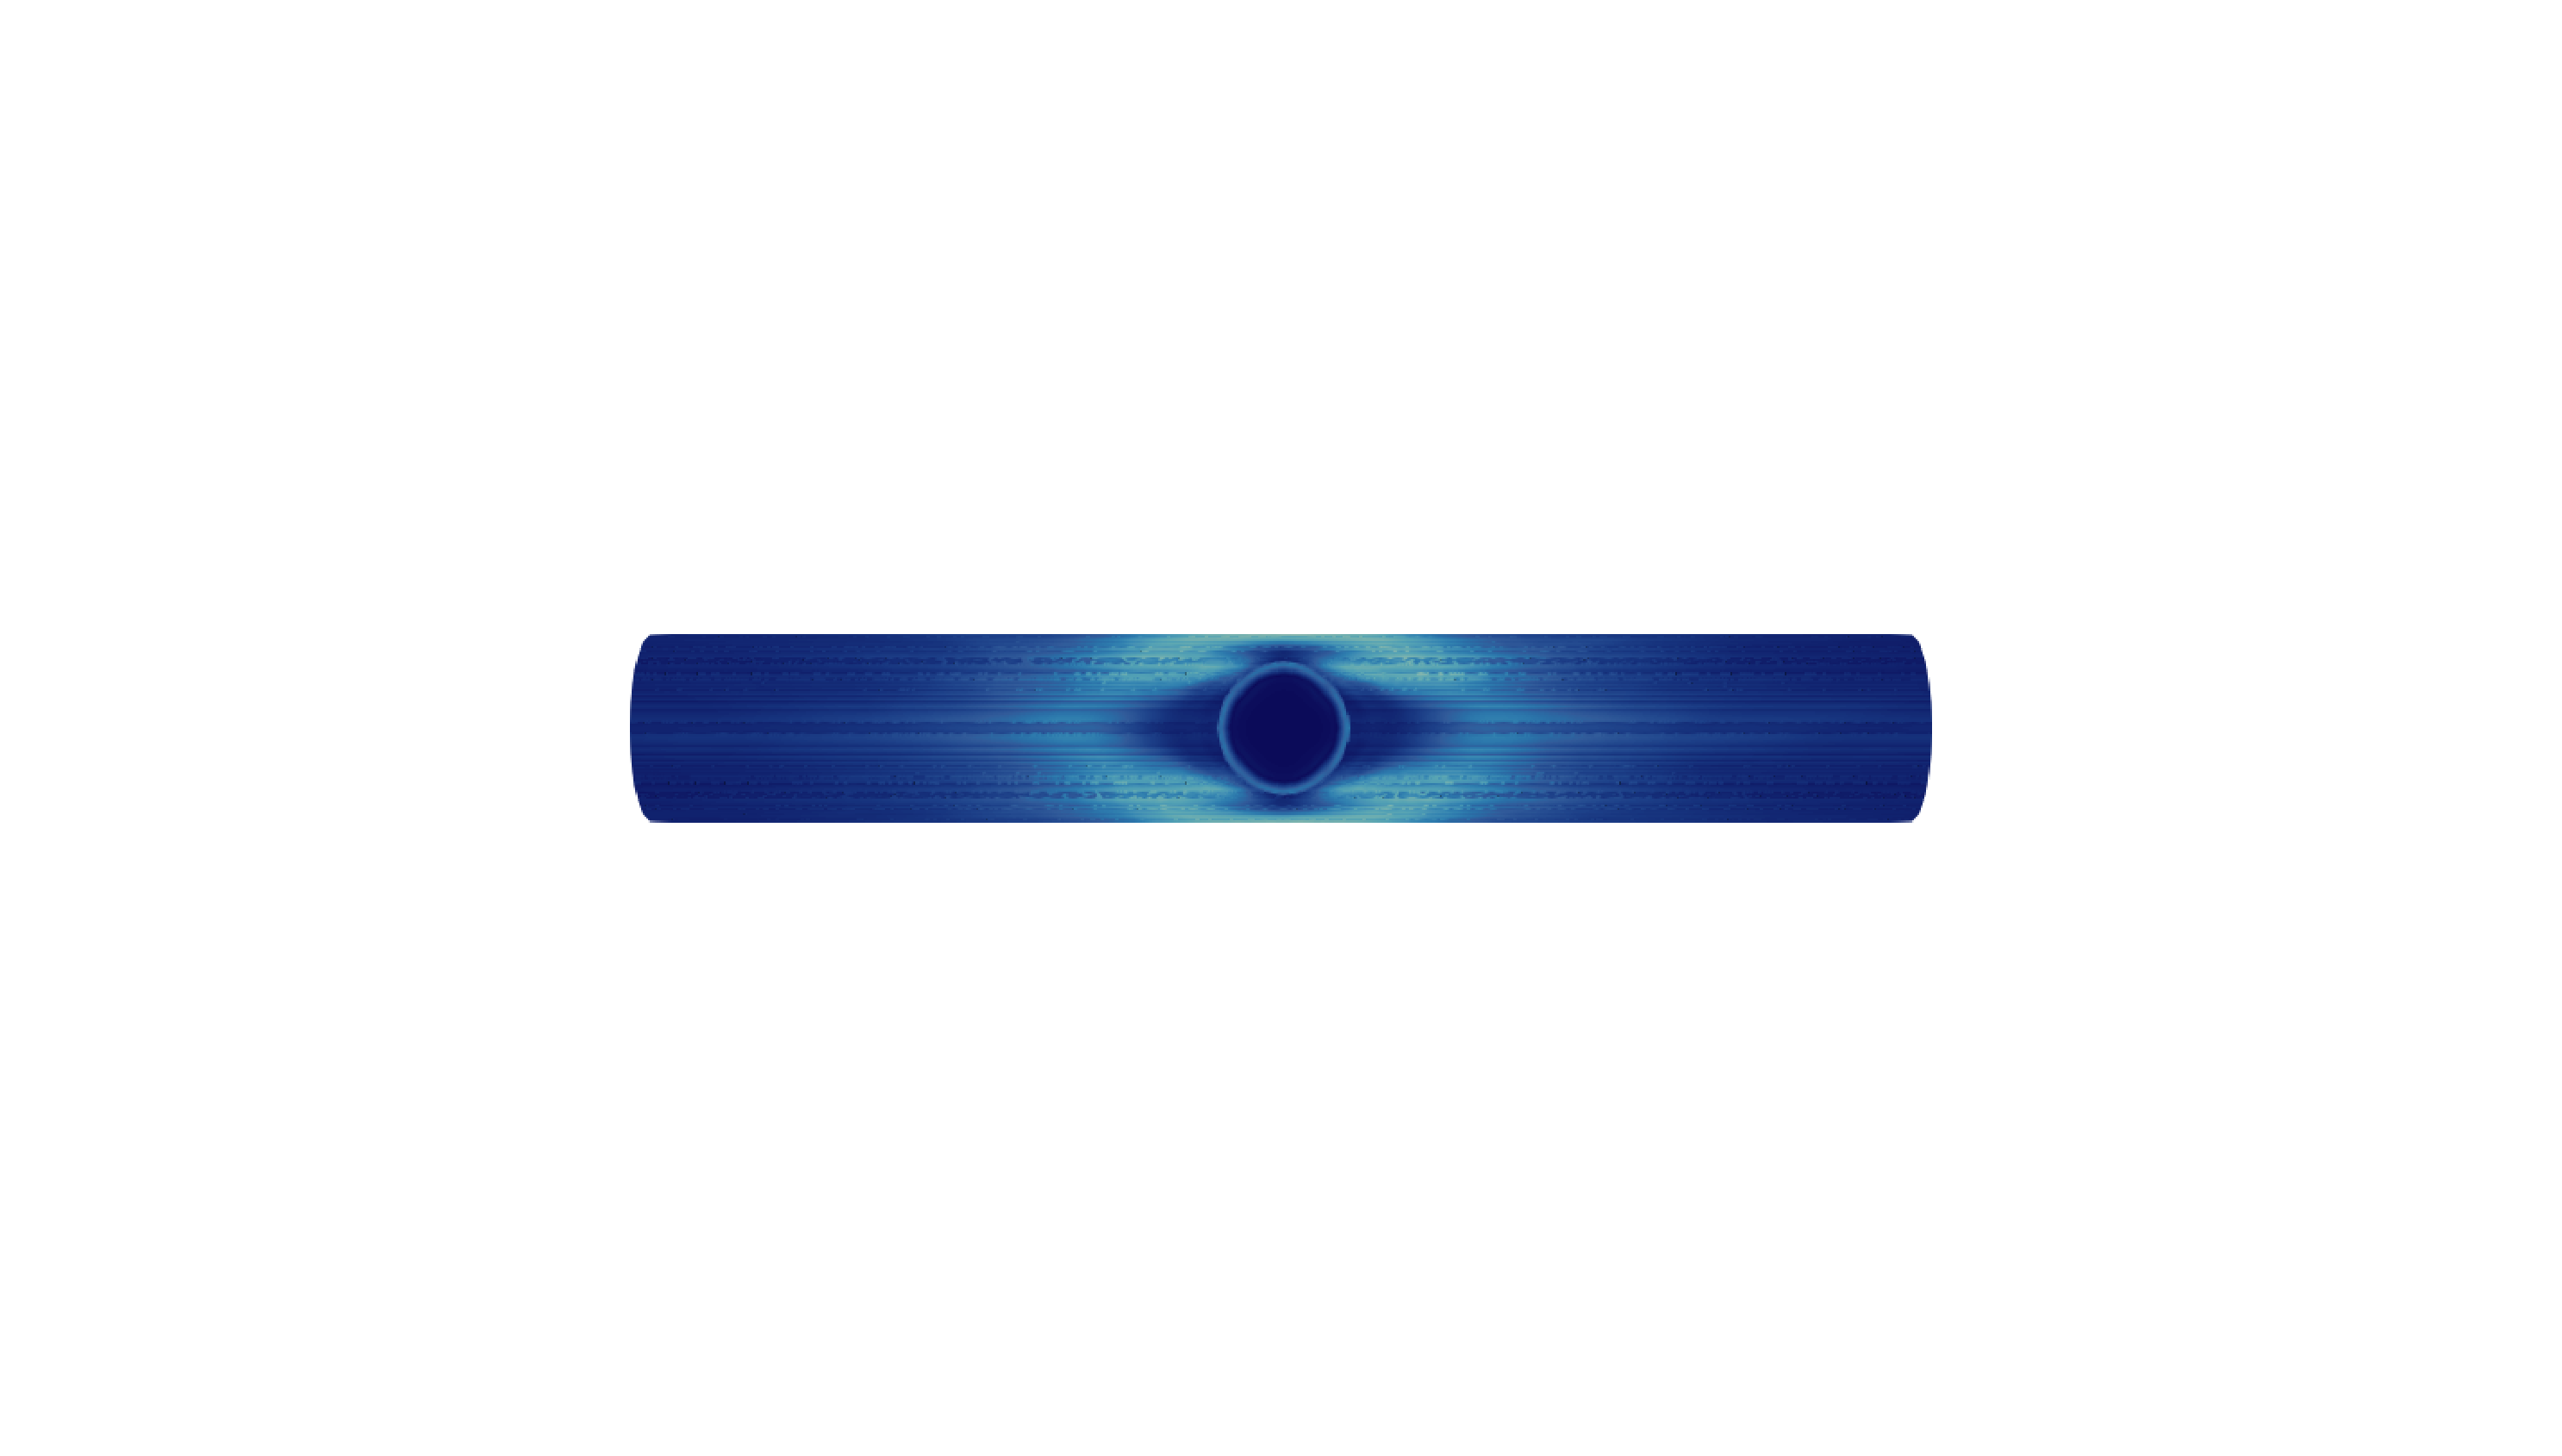
\includegraphics[
		width=\textwidth,
		trim={130mm 85mm 130mm 80mm},
		clip
		]
		{figures/plots/00/00_mean_stress_xy.pdf}%
		\llap{\raisebox{-0.5cm}{%  move next graphics to top right corner
				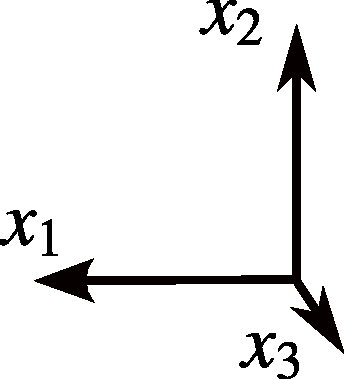
\includegraphics[height=1.5cm]{figures/x1x2x3-top.pdf}%
		}}
		
		
		
\includegraphics[
		width=0.85\textwidth,
		]
		{figures/plots/filler.pdf}
		\caption{Mean shear rate in the \(x_1\)-\(x_2\) plane.}
		\label{fig:mean_stress_xy00}
	\end{subfigure}
	\begin{center}
		\vspace{-32mm}
		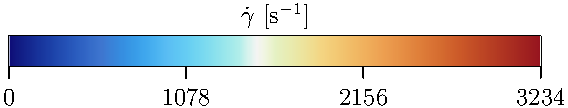
\includegraphics[
		width=0.4\textwidth,
		]
		{figures/plots/mean_stress_leg.pdf}
		
	\end{center}
	
	\vspace{12mm}
	\caption{Mean shear rate visualizations in the \(x_1\)-\(x_3\) and in the \(x_1\)-\(x_2\) plane for the case of point P$_0$, i.e., when $o_1 = 0{,}0 \, \mathrm{cm}$.}
	\label{fig:shear_rate00}
\end{figure}
\vspace{-3mm}
\begin{figure}[H]
	\subsection*{Velocity fluctuations}
	\vspace{-4mm}
	\rule{\textwidth}{0.4pt}\\
	\begin{subfigure}{0.48\textwidth}
		%		\vspace{-2mm}
		\centering
		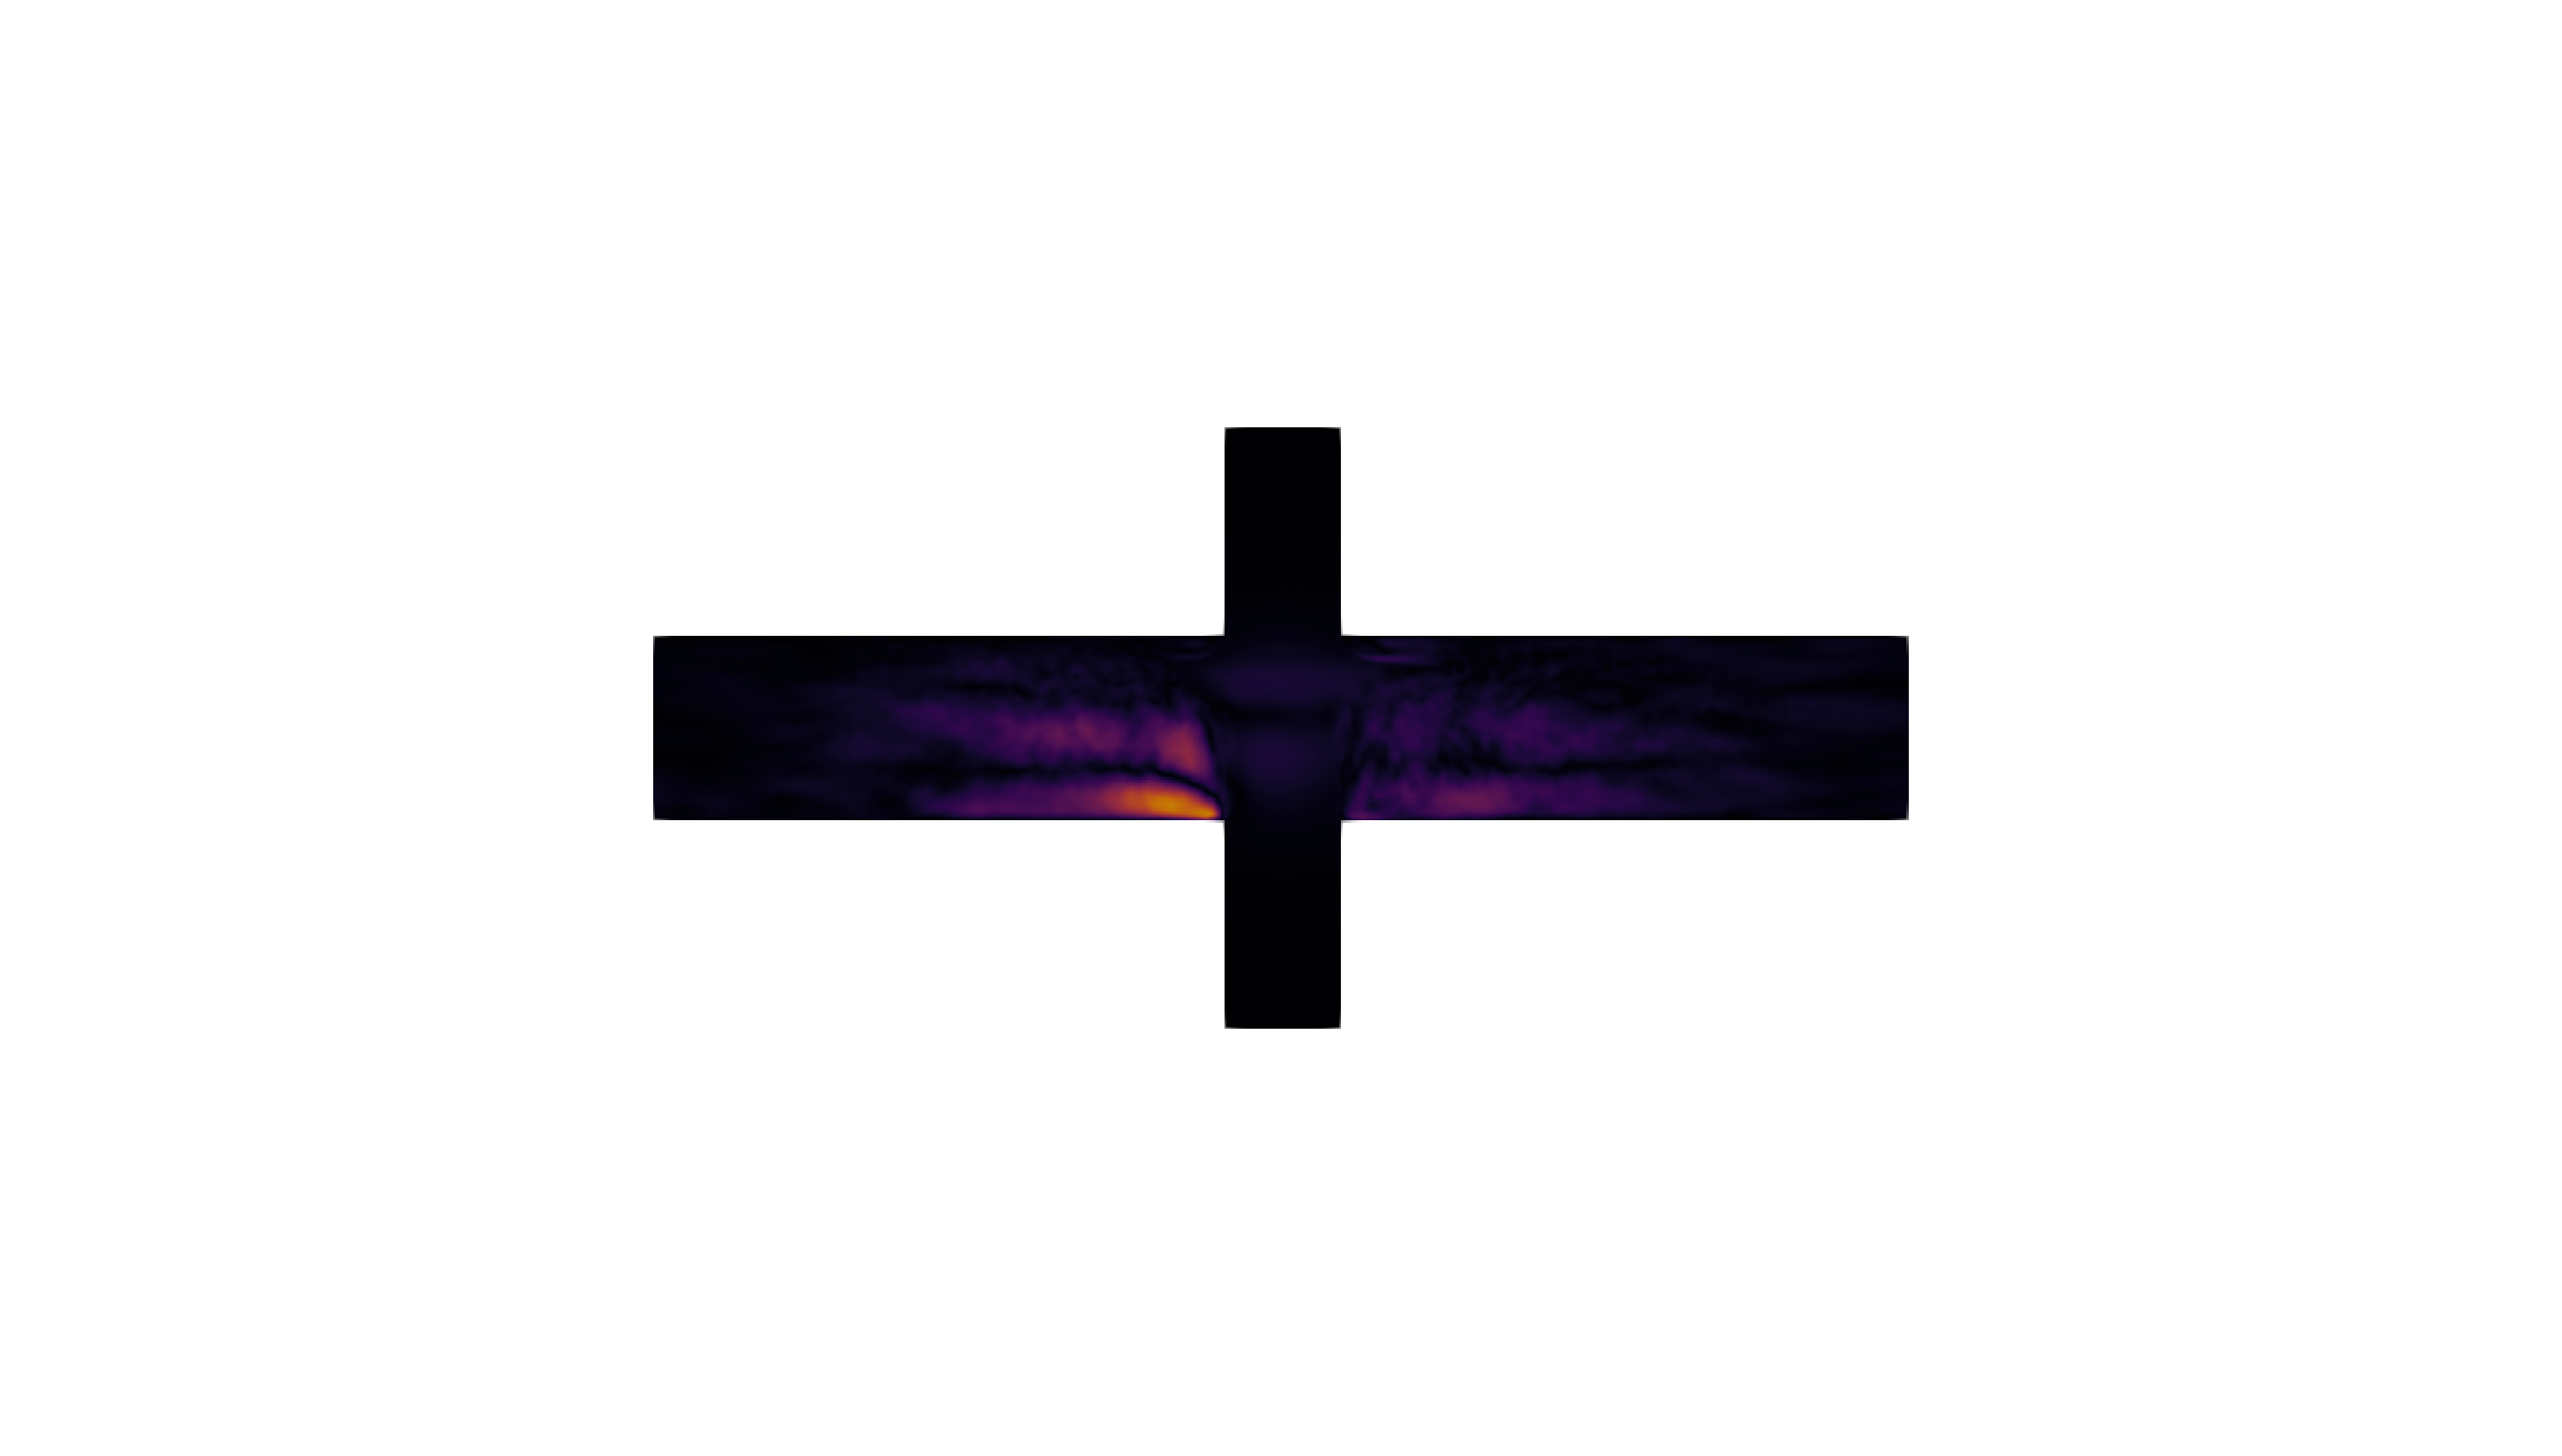
\includegraphics[
		width=\textwidth,
		trim={130mm 85mm 130mm 80mm},
		clip
		]
		{figures/plots/00/00_mean_flucs_xz.pdf}%
		\rlap{\hspace{-7cm}\raisebox{-0.5cm}{%  move next graphics to top right corner
				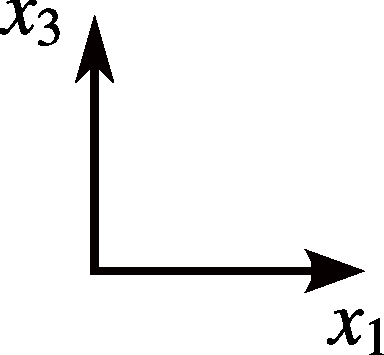
\includegraphics[height=1.5cm]{figures/x1x3.pdf}%
		}}
		
		
\includegraphics[
		width=0.81\textwidth,
		]
		{figures/plots/filler.pdf}
		\caption{Mean velocity fluctuations magnitude field in the \(x_1\)-\(x_3\) plane.}
		\label{fig:mean_flucs_xz00}
		
	\end{subfigure}\hfill%
	\begin{subfigure}{0.48\textwidth}
		\vspace{-1mm}
		\centering
		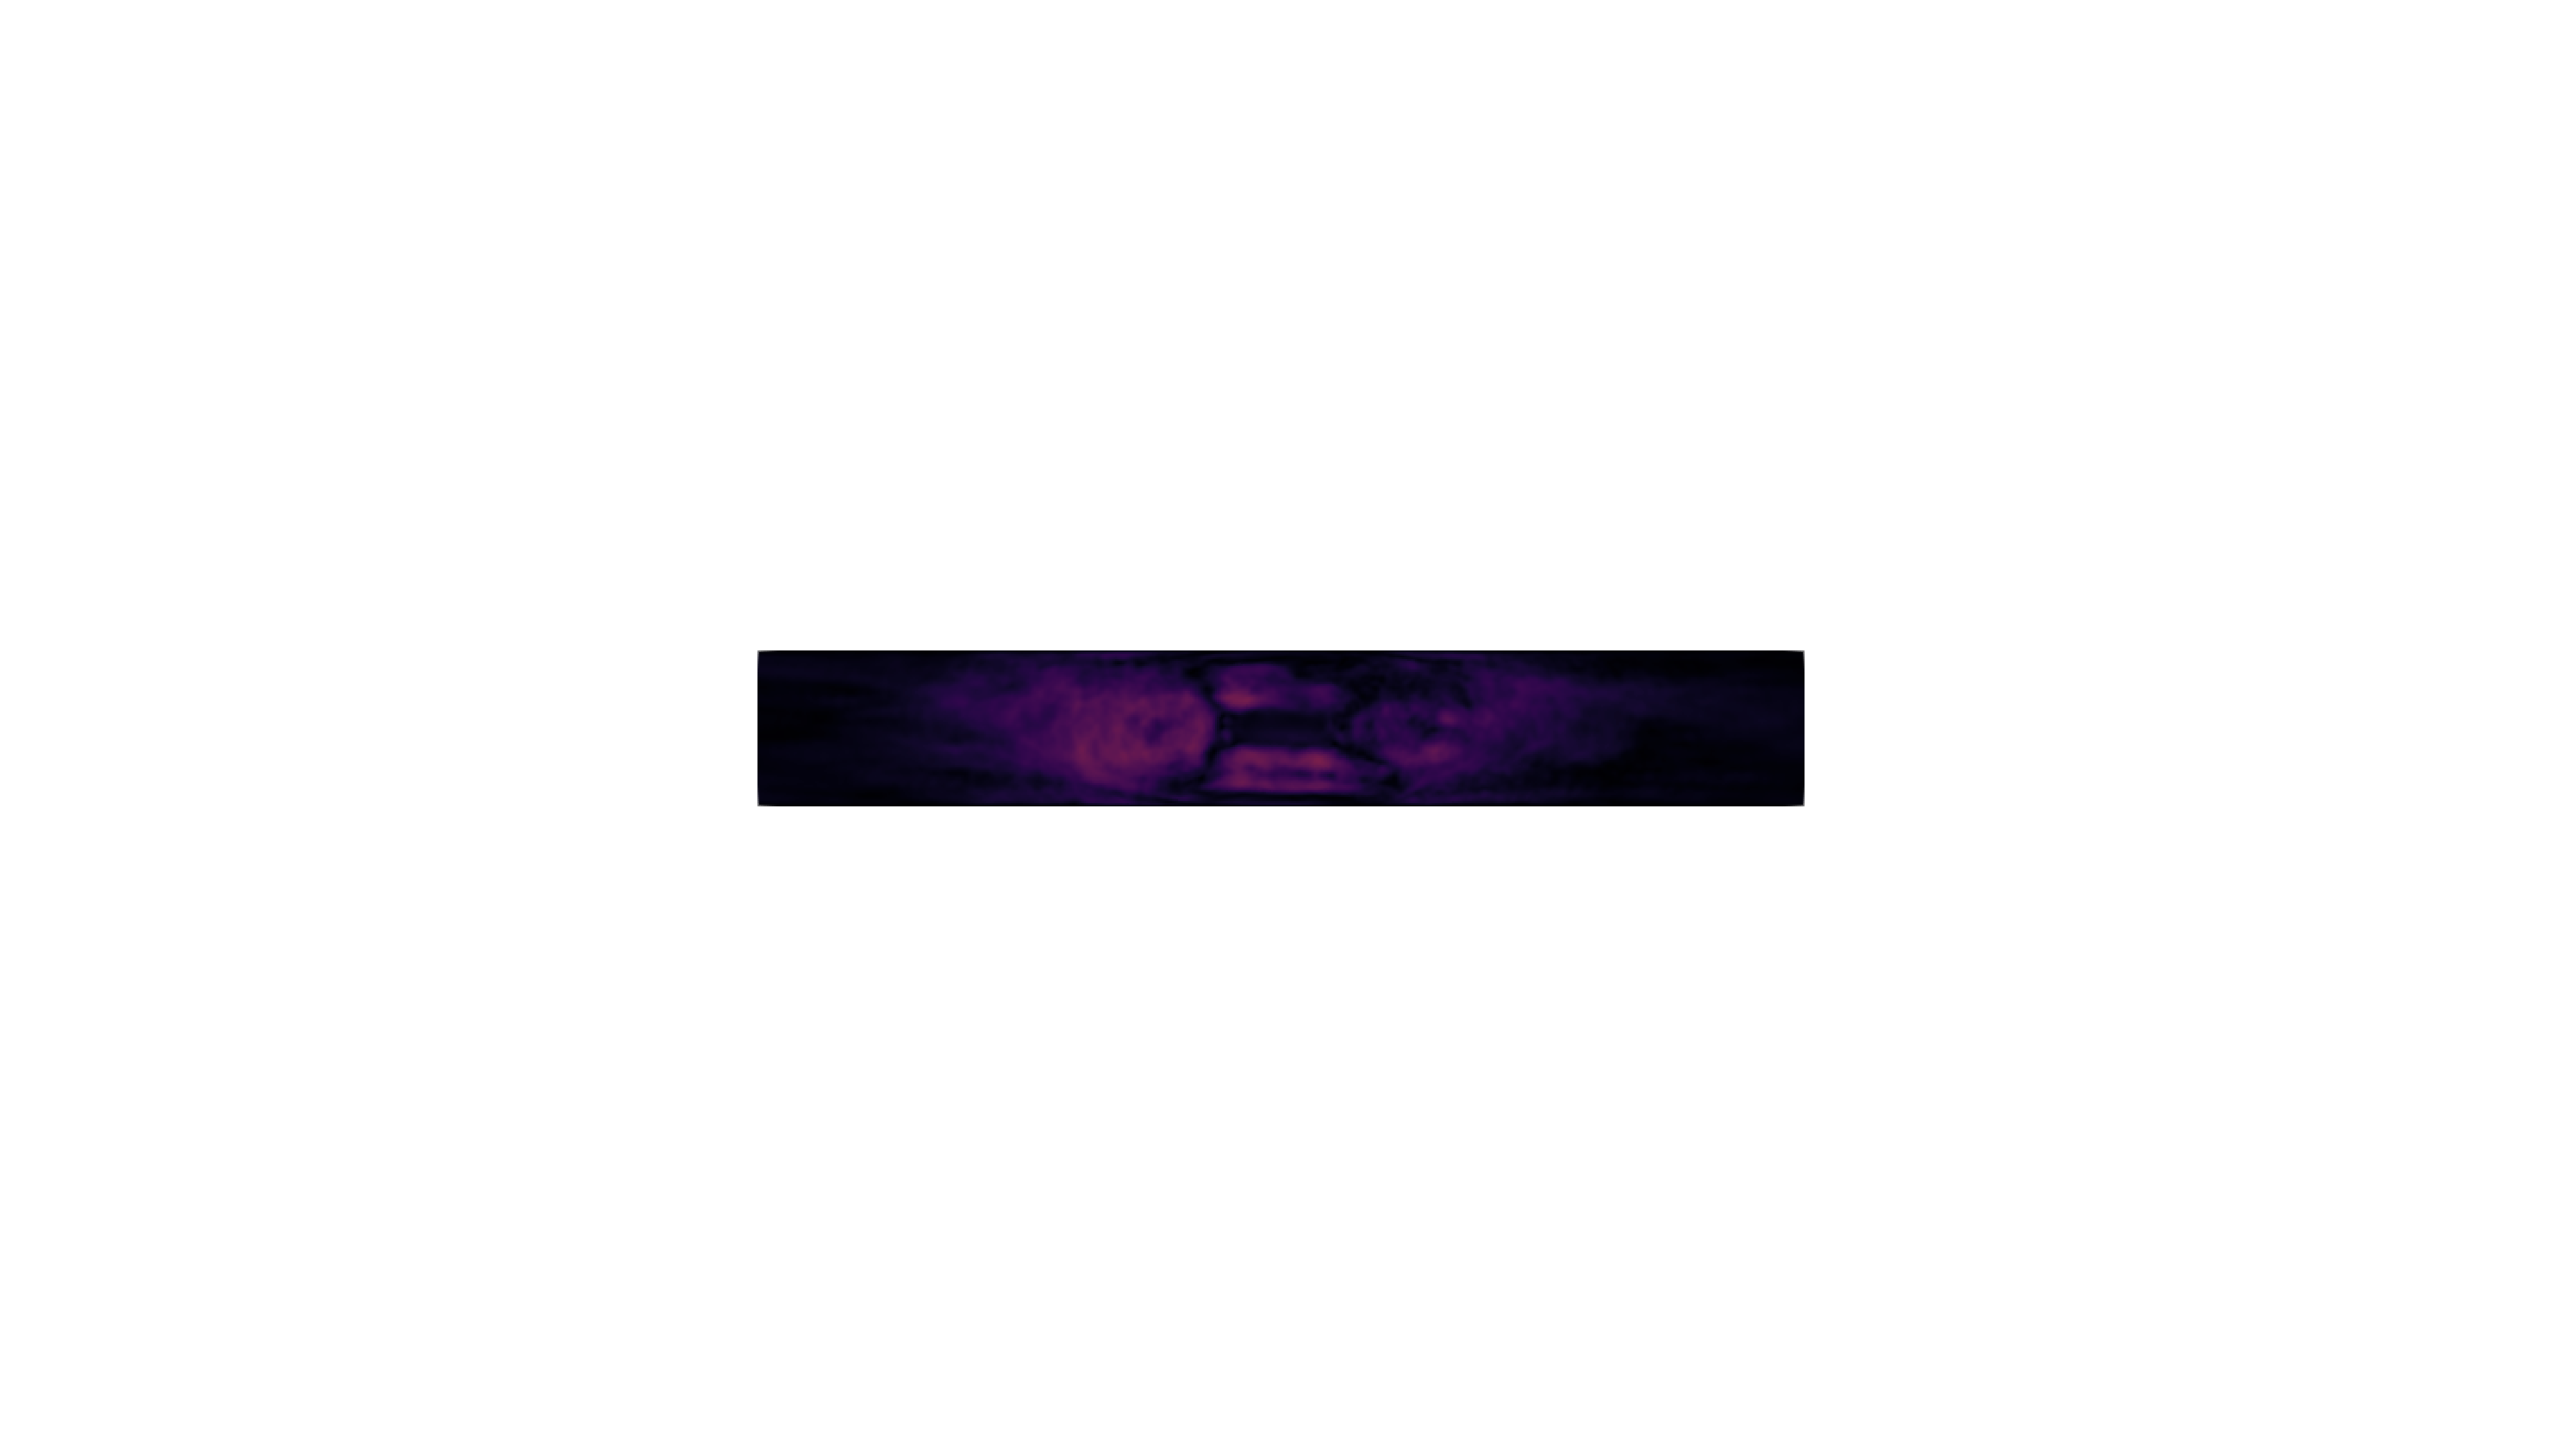
\includegraphics[
		width=1.06\textwidth,
		trim={130mm 98mm 130mm 85mm},
		clip
		]
		{figures/plots/00/00_mean_flucs_xy.pdf}%
		\rlap{\hspace{-1.9cm}\raisebox{-0.7cm}{%  move next graphics to top right corner
				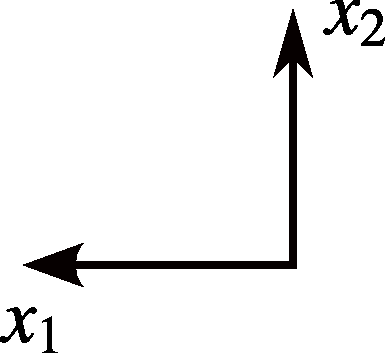
\includegraphics[height=1.5cm]{figures/x1x2.pdf}}}
		
		
		
\includegraphics[
		width=0.81\textwidth,
		]
		{figures/plots/filler.pdf}
		\caption{Mean velocity fluctuations magnitude field in the \(x_1\)-\(x_2\) plane.}
		\label{fig:mean_flucs_xy00}
	\end{subfigure}
	\begin{center}
		\vspace{-32mm}
		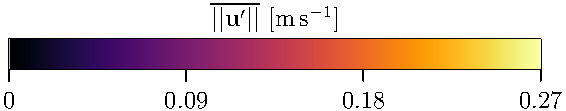
\includegraphics[
		width=0.4\textwidth,
		]
		{figures/plots/mean_flucs_leg.pdf}
		
	\end{center}
	
	\vspace{12mm}
	\caption{Mean velocity fluctuations in the \(x_1\)-\(x_3\) and in the \(x_1\)-\(x_2\) plane for the case when $o_1 = 0{,}0 \, \mathrm{cm}$.}
	\label{fig:velocity_fluctuations00}
\end{figure}
\vspace{-3mm}
\begin{figure}[H]
	\subsection*{SVC/IVC split}
	\vspace{-3mm}
	\rule{\textwidth}{0.4pt}
	\begin{subfigure}{0.60\textwidth}
		\vspace{0mm}
		\centering
		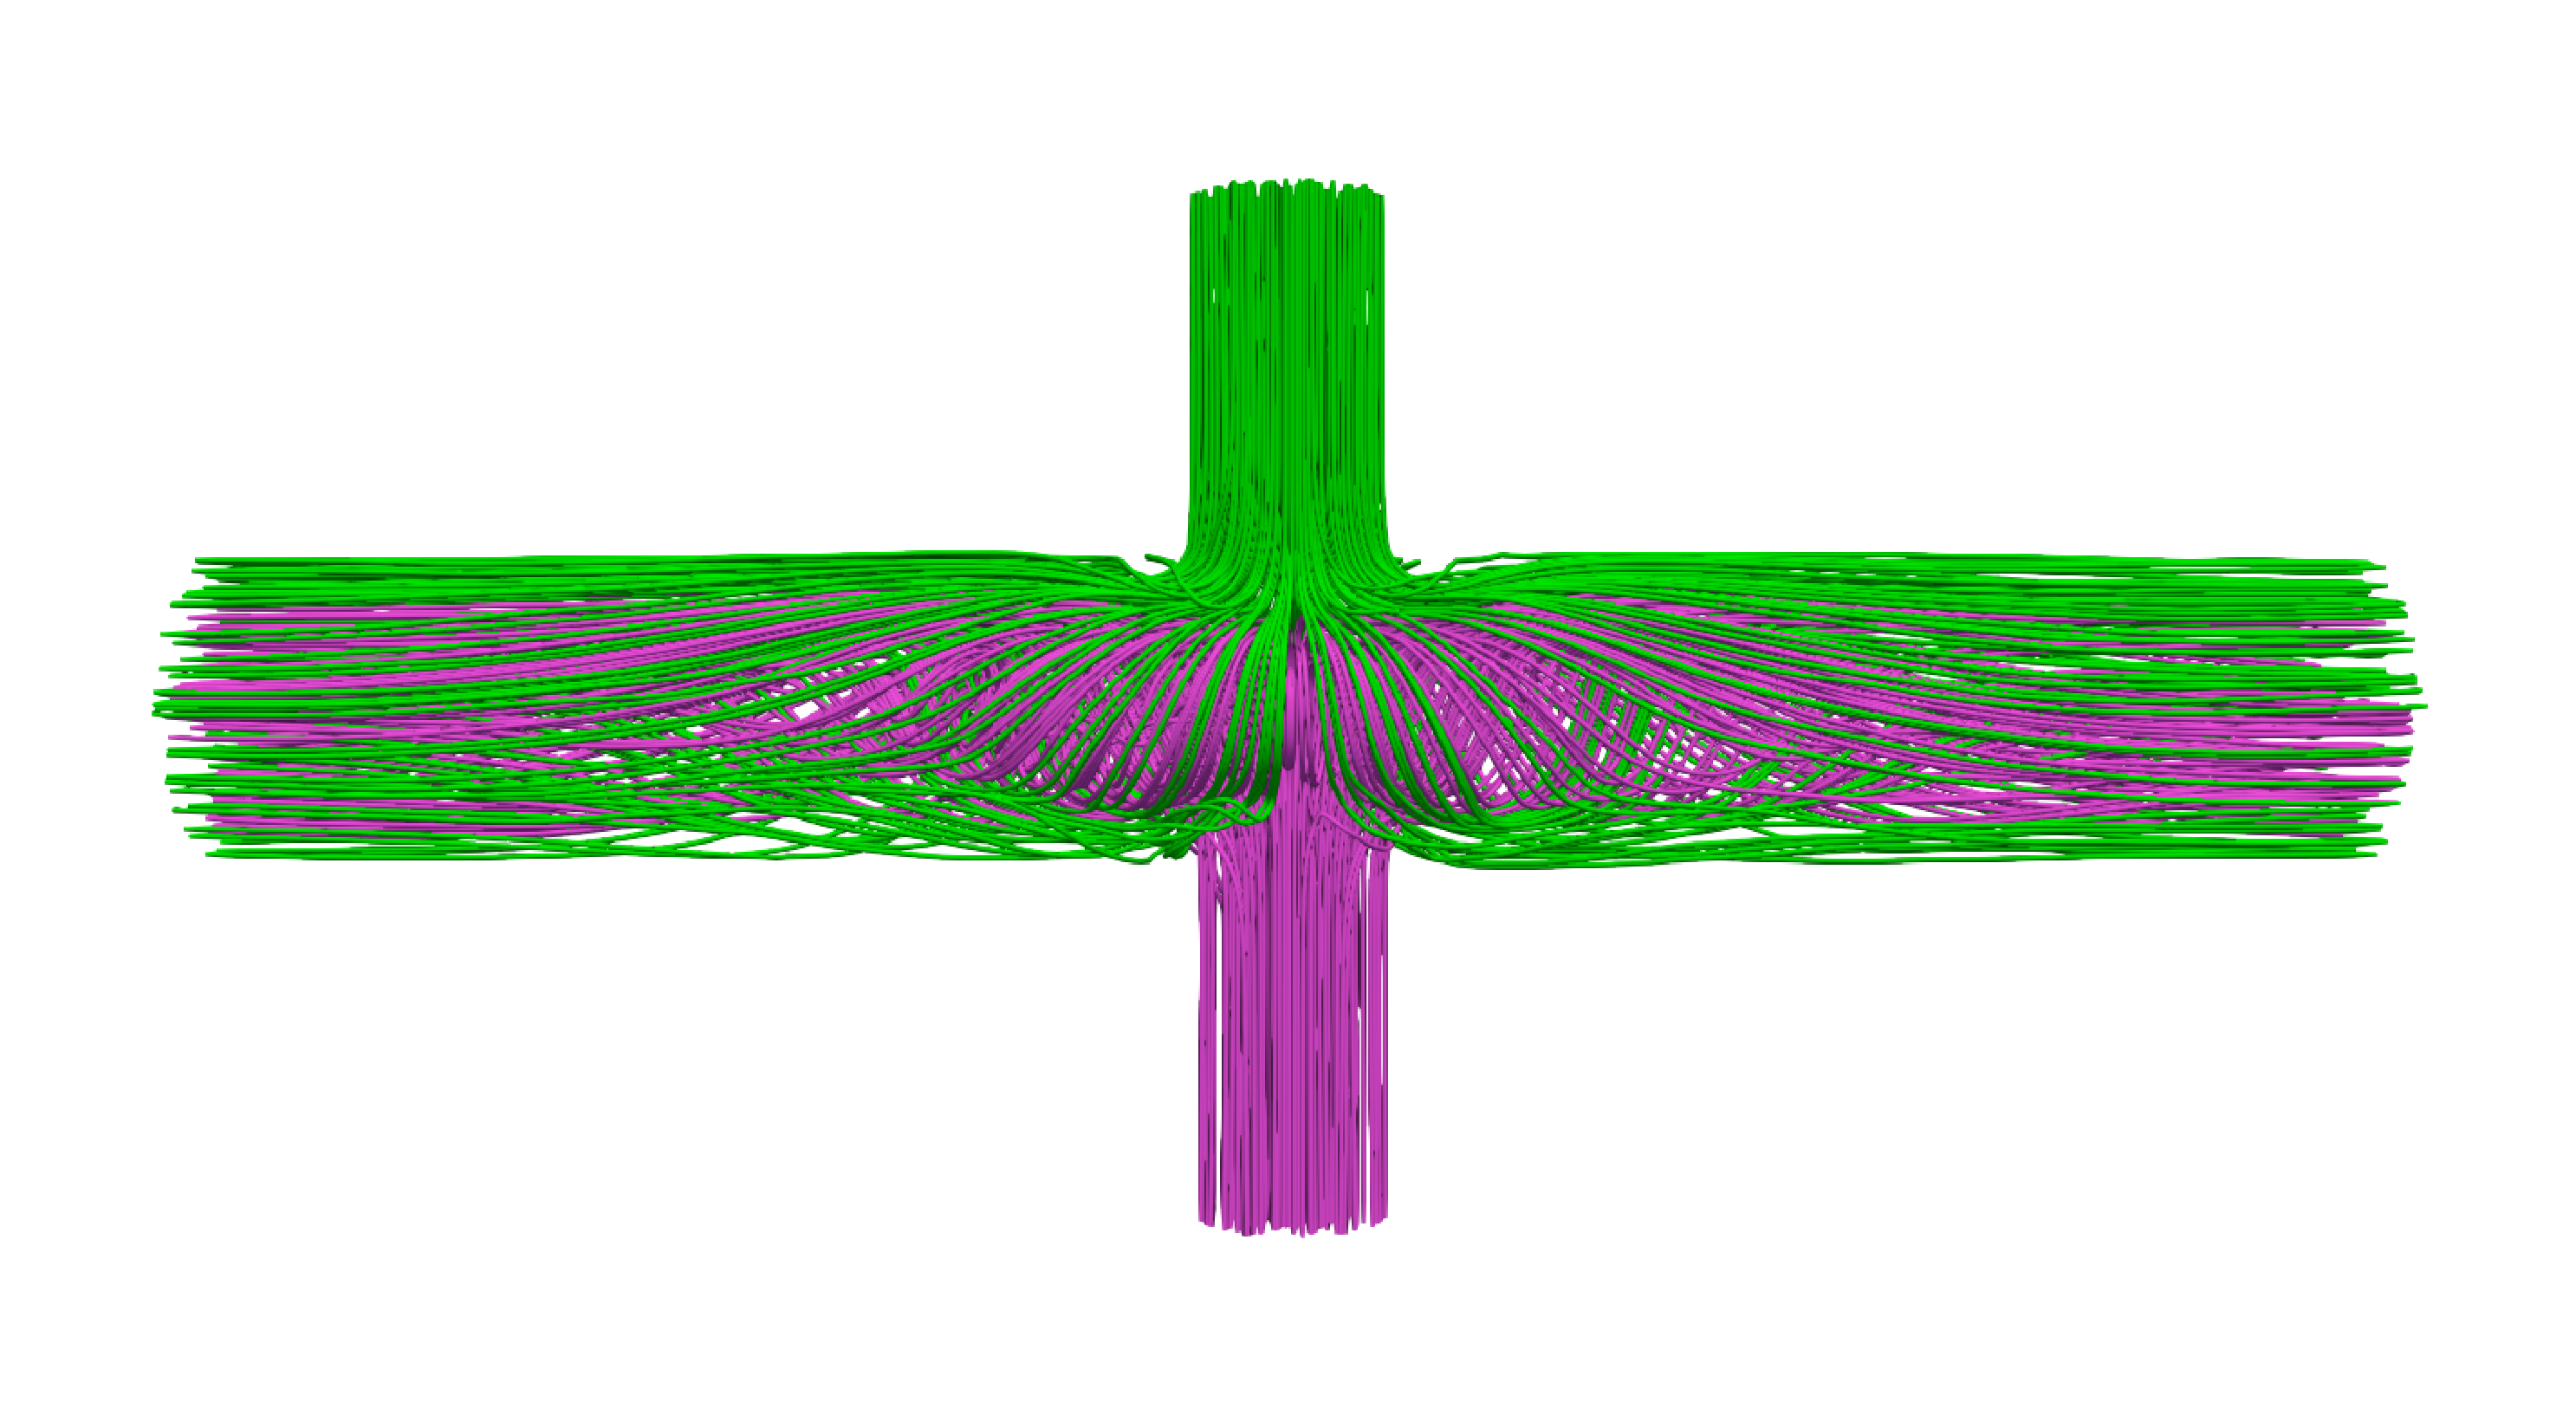
\includegraphics[
		width=\textwidth,
		trim={10mm 10mm 10mm 26mm},
		clip
		]
		{figures/plots/00/00_lpa_rpa_split.pdf}%
		\rlap{\hspace{-8.6cm}\raisebox{-0.0cm}{%  move next graphics to top right corner
				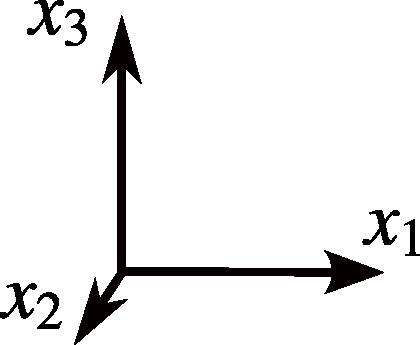
\includegraphics[height=1.5cm]{figures/x1x2x3-side.pdf}%
		}}
		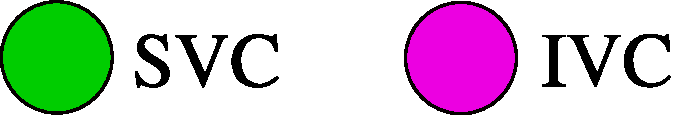
\includegraphics[
		width=0.3\textwidth,
		]
		{figures/plots/split_leg.pdf}
		%			\caption{Placeholder caption.}
	\end{subfigure}\hfill%
	\begin{subfigure}{0.38\textwidth}
		\hspace{7mm}
		\bgroup
		\centering
		\vspace{-0mm}
		\setlength\tabcolsep{3mm}
		\def\arraystretch{1.9}%
		\begin{tabular}{|c|c|c|}
			\hline
			& RPA & LPA \\ \hline
			SVC & 51{,}38\% & 48{,}62\% \\ \hline
			IVC & 50{,}76\% & 49{,}24\% \\ \hline
		\end{tabular}
		%			\caption{Distribution of fluid sources to RPA and LPA.}
		\label{tab:fluid_distribution00}
		\egroup
	\end{subfigure}
	
	\vspace{2mm}
	\caption{Analysis of the split between the SVC and IVC contributions to the LPA and the RPA for the case of point P$_0$, i.e., when $o_1 = 0{,}0 \, \mathrm{cm}$. The figure illustrates the flow split, and the table provides the exact percentages.}
	\label{fig:svc_ivc_split00}
\end{figure}
\vspace{-7mm}
\restoregeometry
\vfill
\section*{Point P$_\mathbf{7}$($o_1=0{,}7 \, \mathrm{ cm}$)}
\begin{figure}[H]
	
	\subsection*{Mean velocities}
	\vspace{-3mm}
	\rule{\textwidth}{0.4pt}
	
	\begin{subfigure}{0.60\textwidth}
		\centering
		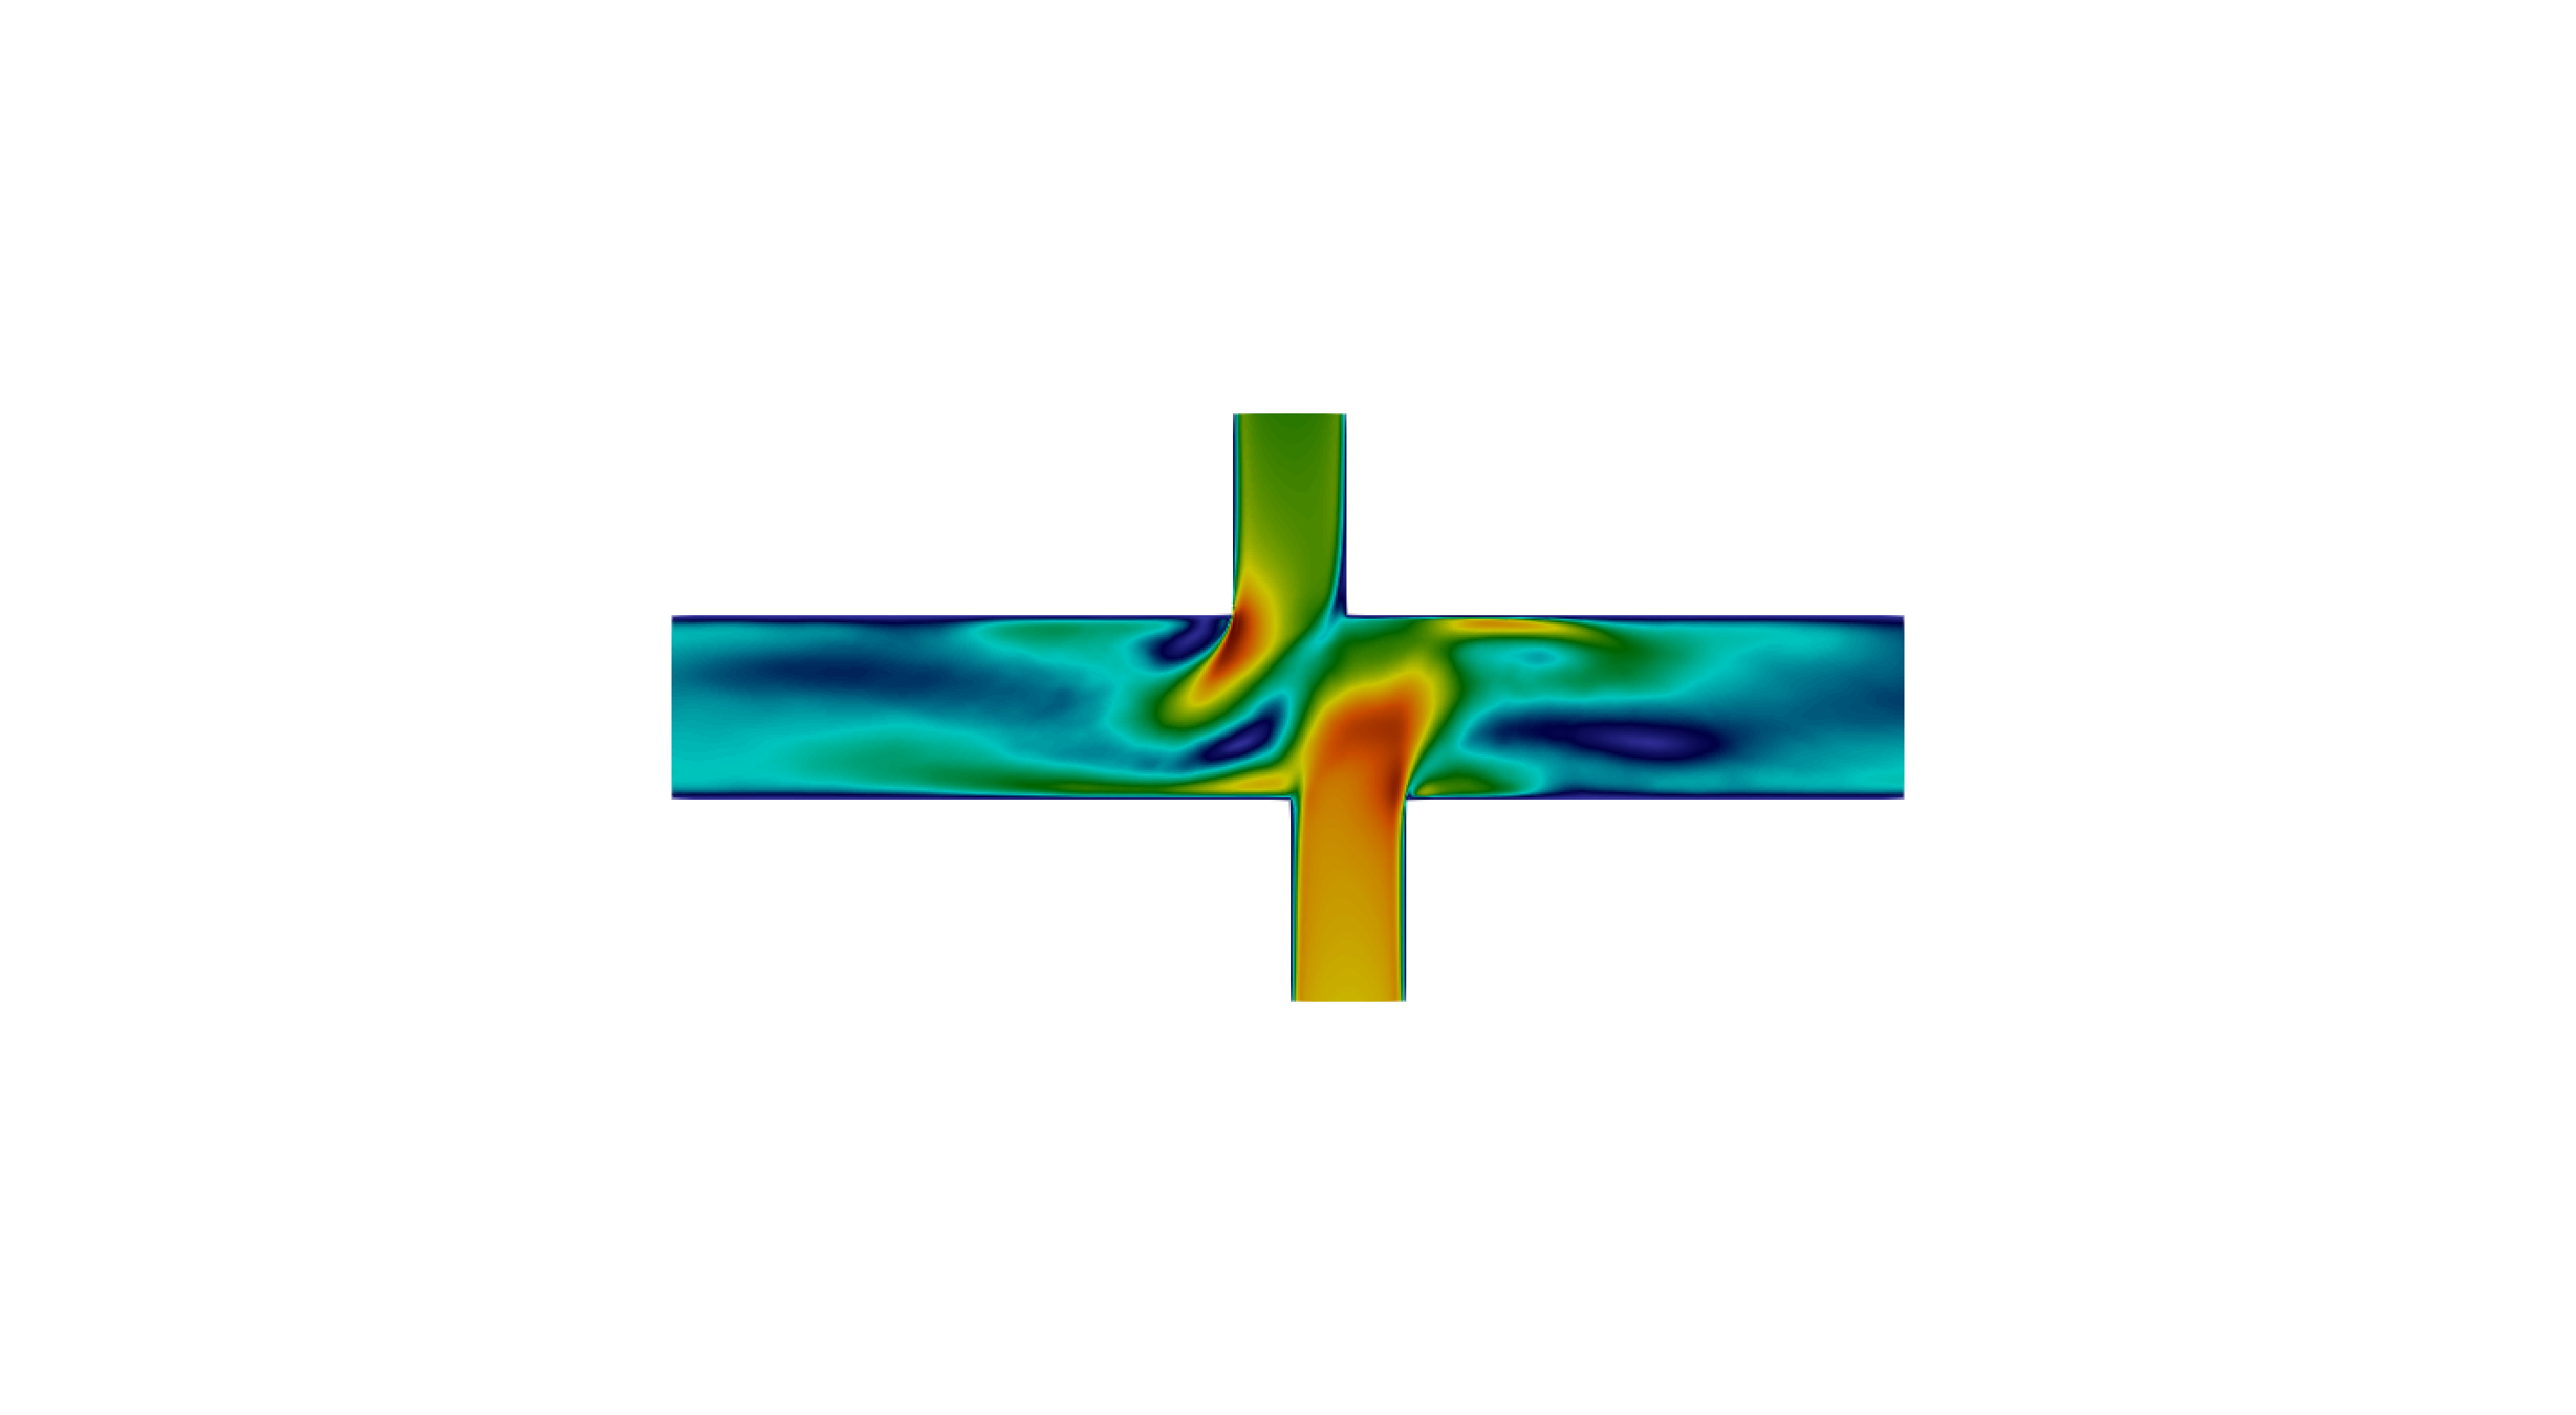
\includegraphics[
		width=\textwidth,
		trim={130mm 70mm 130mm 70mm},
		clip
		]
		{figures/plots/07/compressed/07_mean_veloc_xz.pdf}%
		\rlap{\hspace{-9.5cm}\raisebox{-0.0cm}{%  move next graphics to top right corner
				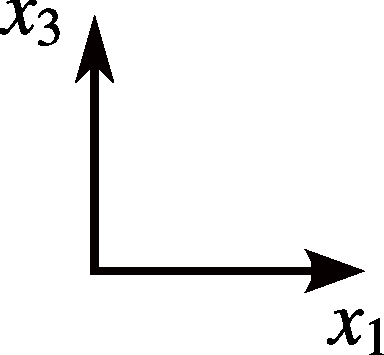
\includegraphics[height=1.5cm]{figures/x1x3.pdf}%
		}}
		
		
\includegraphics[
		width=0.85\textwidth,
		]
		{figures/plots/filler.pdf}
		\caption{Mean velocity magnitude field in the \(x_1\)-\(x_3\) plane.}
		\label{fig:mean_velocity_xz07}
		
	\end{subfigure}\hfill%
	\begin{subfigure}{0.36\textwidth}
		\vspace{14mm}
		\centering
		LPA\hspace{24mm}RPA
		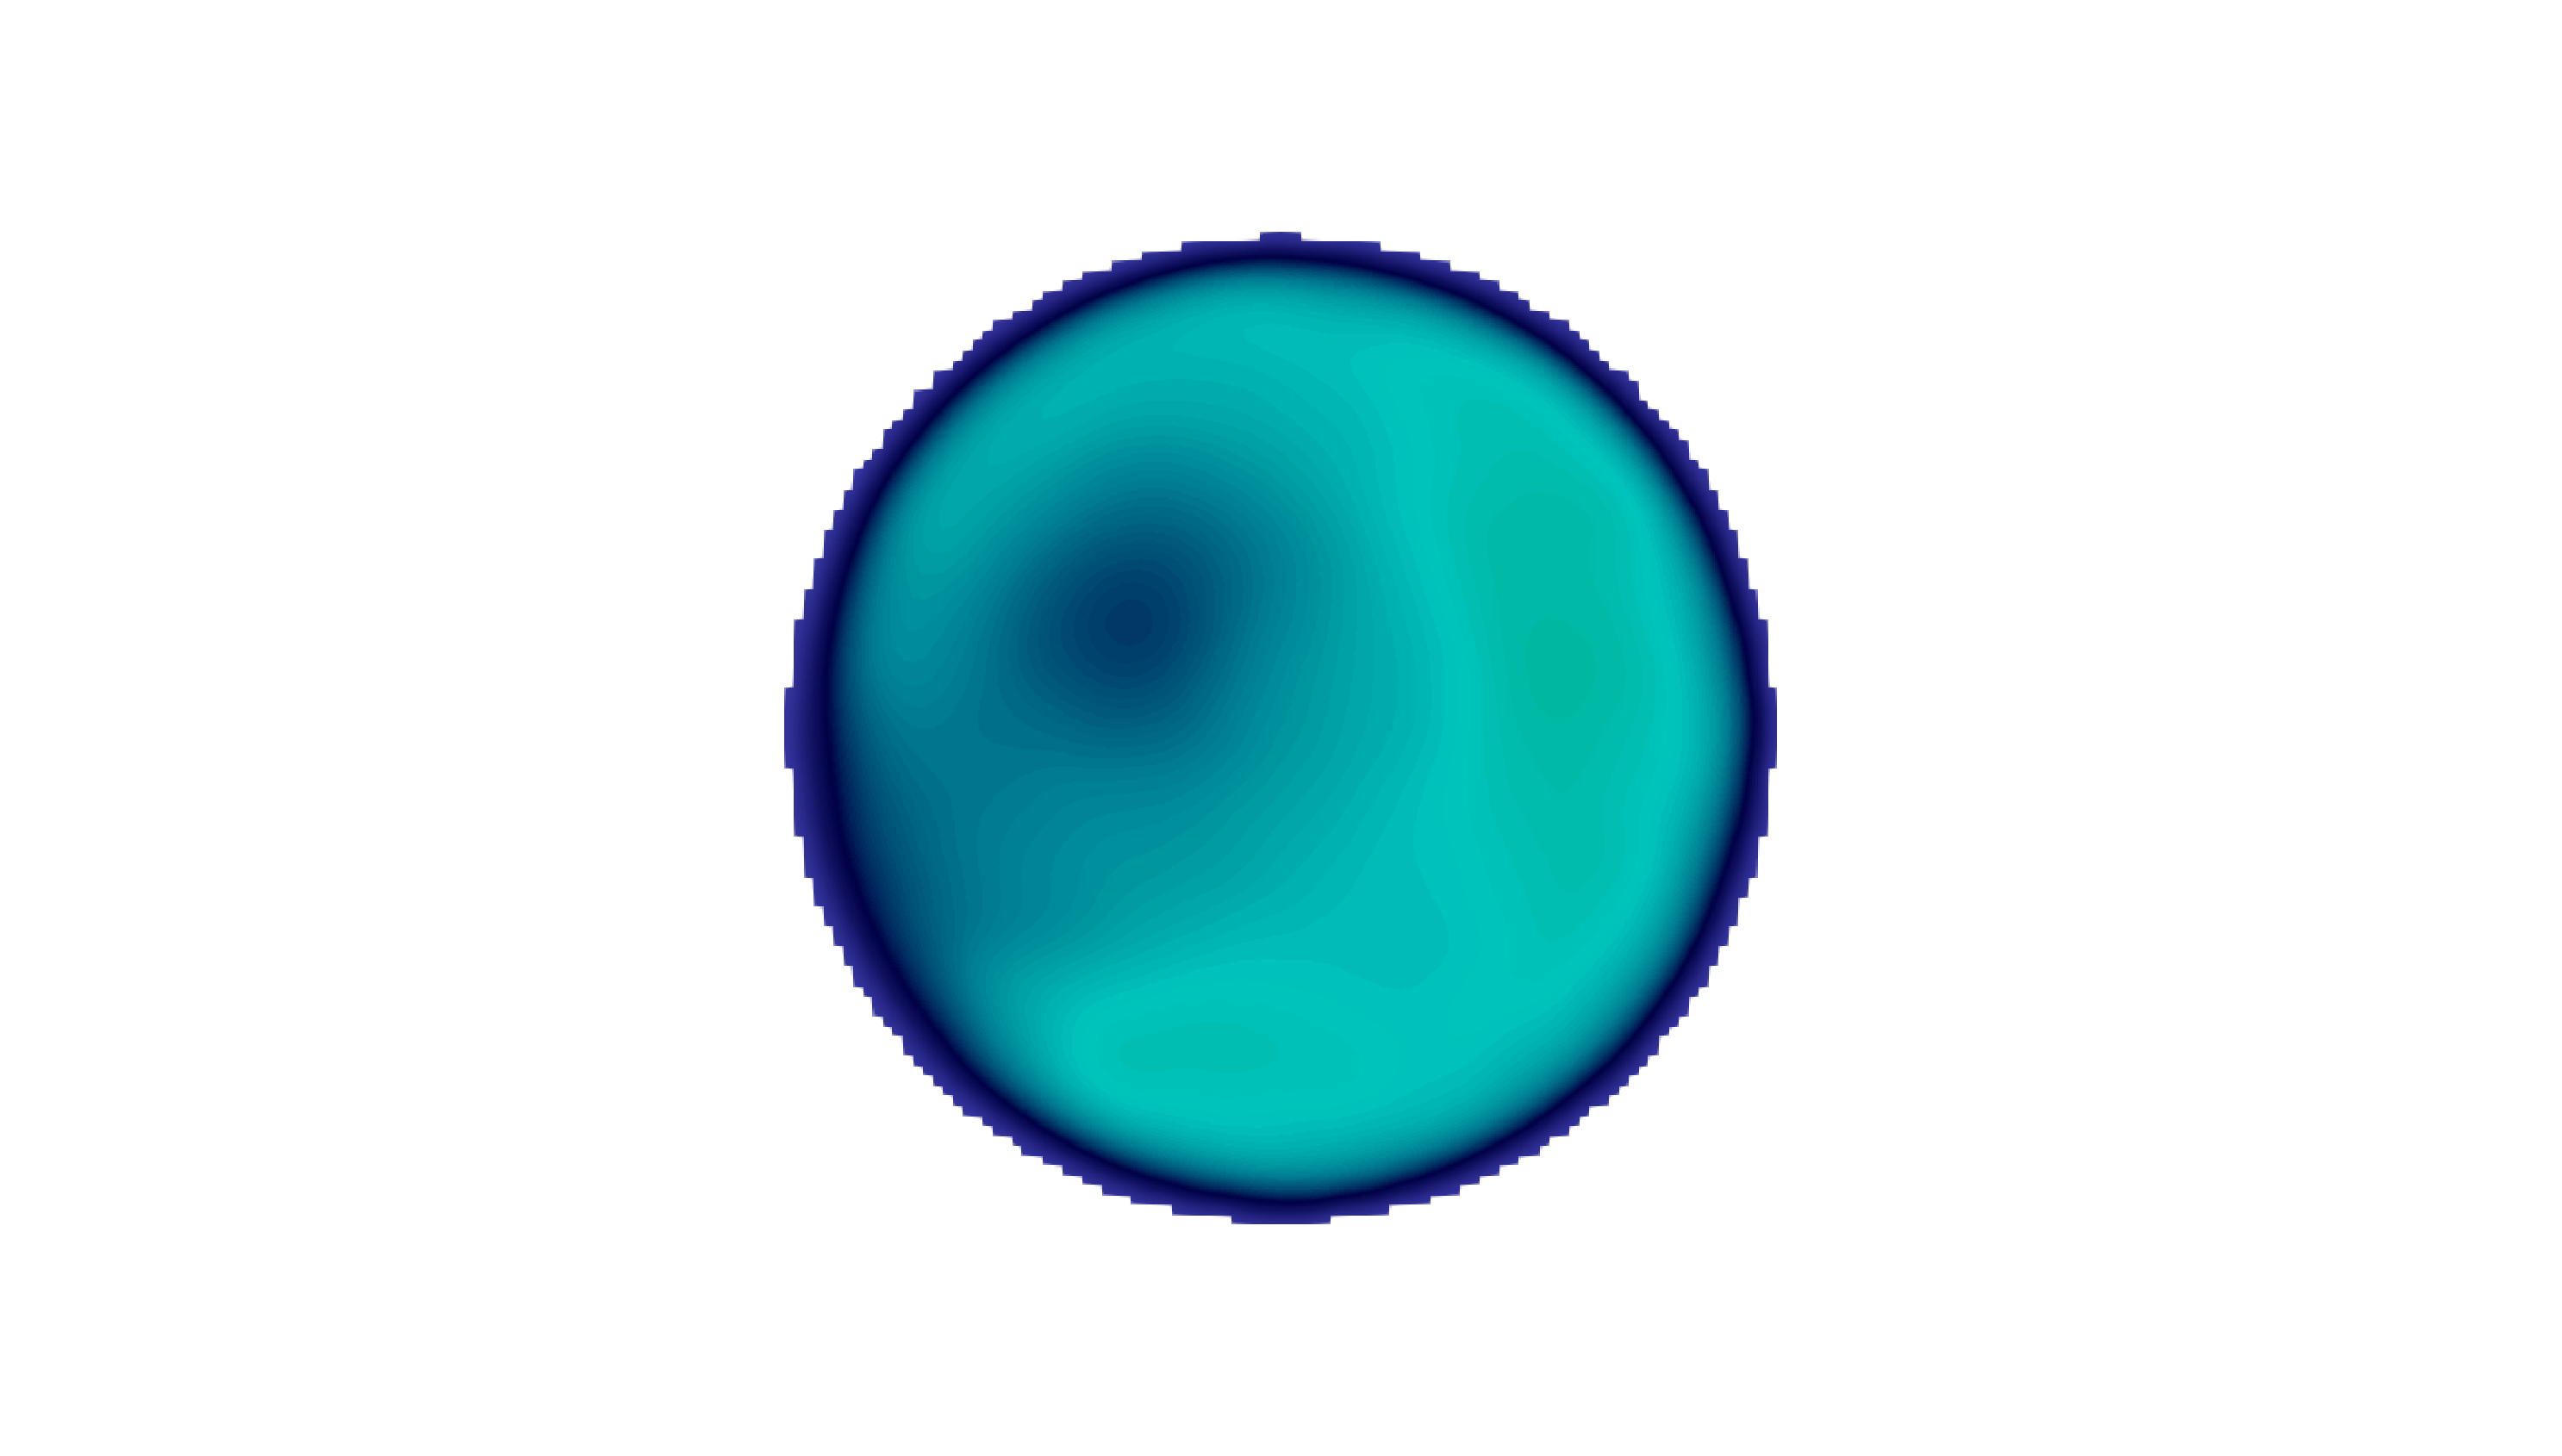
\includegraphics[
		width=0.46\textwidth,
		trim={150mm 20mm 150mm 20mm},
		clip
		]
		{figures/plots/07/compressed/07_LPA_mean_veloc.pdf}\hfill
		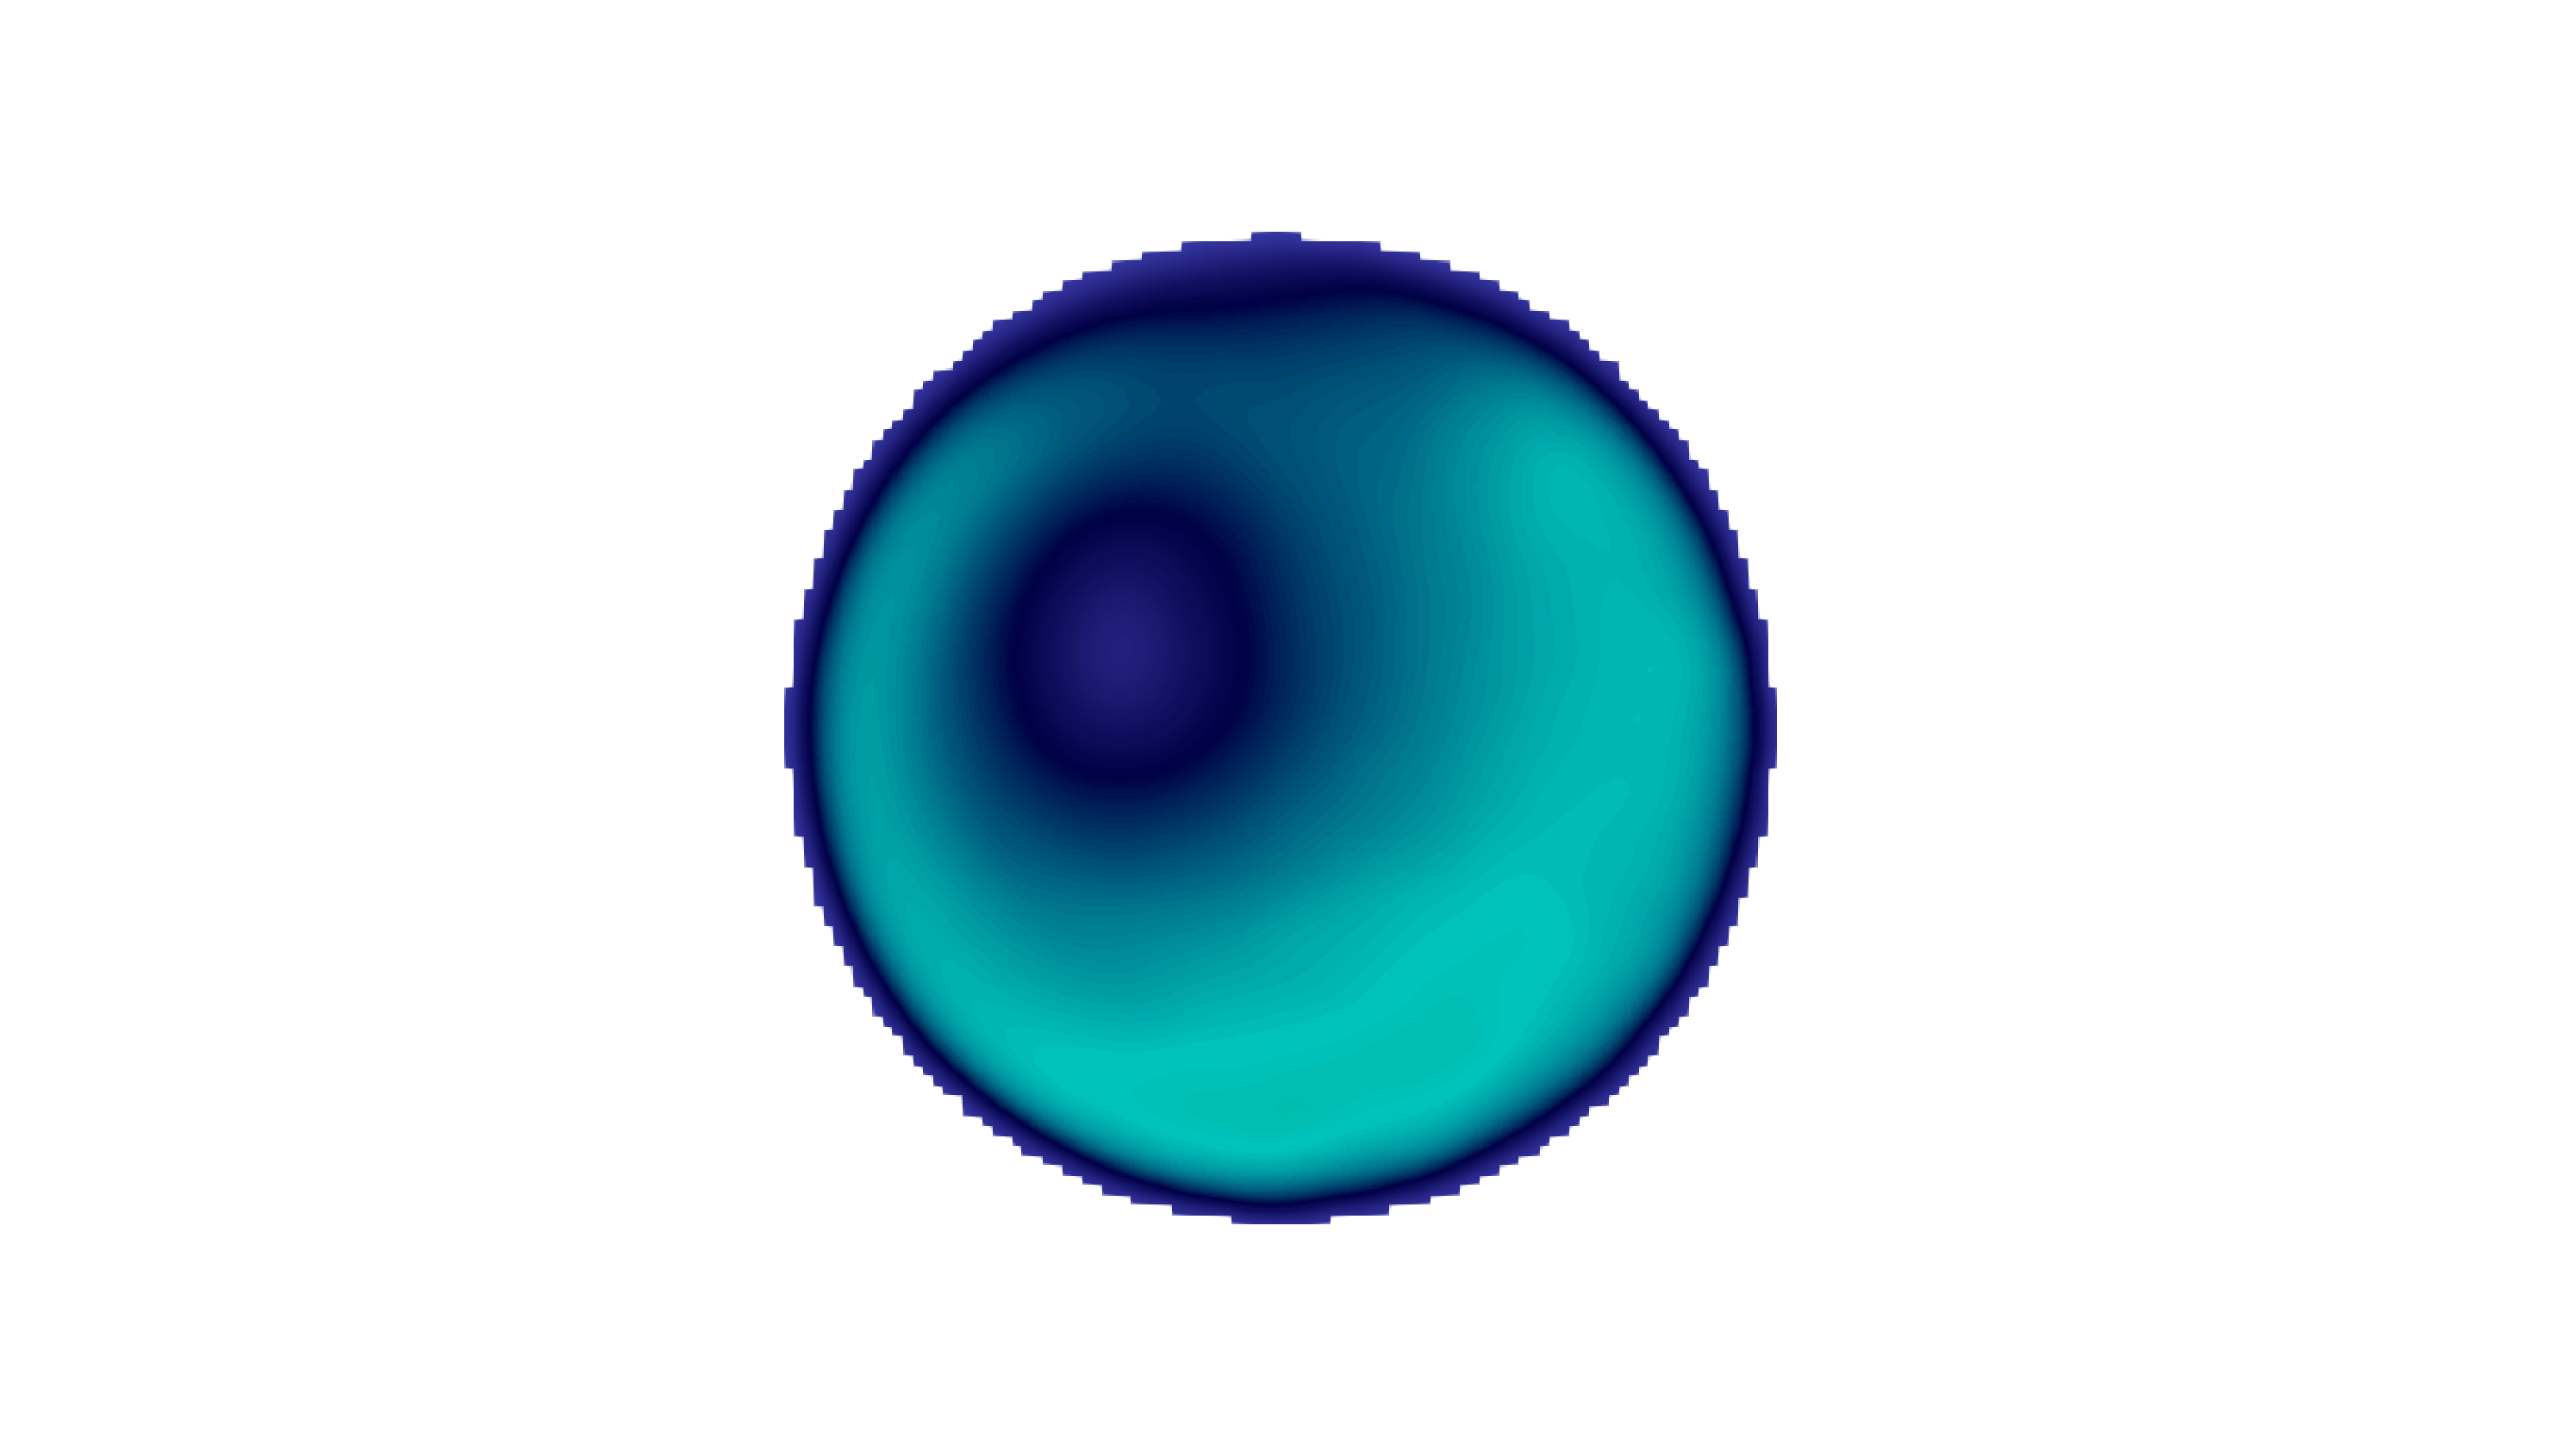
\includegraphics[
		width=0.46\textwidth,
		trim={150mm 20mm 150mm 20mm},
		clip
		]
		{figures/plots/07/compressed/07_RPA_mean_veloc.pdf}\\[38pt]
		
		
\includegraphics[
		width=1.08\textwidth,
		]
		{figures/plots/filler.pdf}
		\caption{Magnitudes of mean velocity at the outlets \(\Gamma^{\text{LPA}}_{\text{out}}\) and \(\Gamma^{\text{RPA}}_{\text{out}}\).}
		\label{fig:mean_velocity_outlets07}
	\end{subfigure}
	\begin{center}
		\vspace{-30mm}
		\includegraphics[
		width=0.4\textwidth,
		]
		{figures/plots/mean_veloc_leg.pdf}
		
	\end{center}
	\vspace{14mm}
	
	\begin{subfigure}{0.60\textwidth}
		\centering
		\includegraphics[
		width=\textwidth,
		trim={10mm 10mm 10mm 10mm},
		clip
		]
		{figures/plots/07/compressed/07_mean_veloc_streamlines.pdf}%
		\rlap{\hspace{-9cm}\raisebox{0.1cm}{%  move next graphics to top right corner
				\includegraphics[height=1.5cm]{figures/x1x2x3.pdf}%
		}}
		\includegraphics[
		width=0.65\textwidth,
		]
		{figures/plots/mean_veloc_leg.pdf}
		\caption{Streamlines of the mean velocity field illustrating the flow trajectory throughout the geometry.}
		\label{fig:mean_velocity_streamlines07}
	\end{subfigure}\hfill%
	\begin{subfigure}{0.36\textwidth}
		\centering
		\vspace{9mm}
		LPA\hspace{24mm}RPA
		\includegraphics[
		width=0.46\textwidth,
		trim={150mm 20mm 150mm 20mm},
		clip
		]
		{figures/plots/07/compressed/07_LPA_angle.pdf}\hfill
		\includegraphics[
		width=0.46\textwidth,
		trim={150mm 20mm 150mm 20mm},
		clip
		]
		{figures/plots/07/07_RPA_angle.pdf}
		
		\includegraphics[
		width=0.99\textwidth,
		]
		{figures/plots/filler.pdf}
		\includegraphics[
		width=1.05\textwidth,
		]
		{figures/plots/angle_leg.pdf}
		\caption{Angle between the mean velocity vector and the normal direction at the outlets \(\Gamma^{\text{LPA}}_{\text{out}}\) and \(\Gamma^{\text{RPA}}_{\text{out}}\).}
		\label{fig:velocity_angle_outlets07}
	\end{subfigure}
	
	\vspace{2mm}
	\caption{Overview of mean velocity fields and outlet characteristics for the case of point P$_7$, i.e., when $o_1 = 0{,}7 \, \mathrm{cm}$. Subfigure (a) shows the velocity magnitude field, (b) displays outlet-specific velocity magnitudes, (c) presents streamlines of the mean velocity field, and (d) details the angular alignment of velocity vectors with outlet normals.}
	\label{fig:mean_velocity_analysis07}
\end{figure}

\newgeometry{top=1.7cm}

\begin{figure}[H]
	\subsection*{Shear rate}
	\vspace{-3mm}
	\rule{\textwidth}{0.4pt}\\
	\begin{subfigure}{0.48\textwidth}
		%		\vspace{-8mm}
		\centering
		\includegraphics[
		width=\textwidth,
		trim={130mm 85mm 130mm 80mm},
		clip
		]
		{figures/plots/07/compressed/07_mean_stress_xz.pdf}%
		\rlap{\hspace{-7cm}\raisebox{-0.5cm}{%  move next graphics to top right corner
				\includegraphics[height=1.5cm]{figures/x1x2x3-side.pdf}%
		}}
		
		
		\includegraphics[
		width=0.85\textwidth,
		]
		{figures/plots/filler.pdf}
		\caption{Mean shear rate in the \(x_1\)-\(x_3\) plane.}
		\label{fig:mean_stress_xz07}
		
	\end{subfigure}\hfill%
	\begin{subfigure}{0.48\textwidth}
		%		\vspace{-8mm}
		\centering
		\includegraphics[
		width=\textwidth,
		trim={130mm 85mm 130mm 80mm},
		clip
		]
		{figures/plots/07/compressed/07_mean_stress_xy.pdf}%
		\llap{\raisebox{-0.5cm}{%  move next graphics to top right corner
				\includegraphics[height=1.5cm]{figures/x1x2x3-top.pdf}%
		}}
		
		
		\includegraphics[
		width=0.85\textwidth,
		]
		{figures/plots/filler.pdf}
			\caption{Mean shear rate in the \(x_1\)-\(x_2\) plane.}
		\label{fig:mean_stress_xy07}
	\end{subfigure}
	\begin{center}
		\vspace{-32mm}
		\includegraphics[
		width=0.4\textwidth,
		]
		{figures/plots/mean_stress_leg.pdf}
		
	\end{center}
	
	\vspace{12mm}
    \caption{Mean shear rate visualizations in the \(x_1\)-\(x_3\) and in the \(x_1\)-\(x_2\) plane for the case of point P$_7$, i.e., when $o_1 = 0{,}7 \, \mathrm{cm}$.}
	\label{fig:shear_rate07}
\end{figure}
\vspace{-3mm}
\begin{figure}[H]
	\subsection*{Velocity fluctuations}
	\vspace{-4mm}
	\rule{\textwidth}{0.4pt}\\
	\begin{subfigure}{0.48\textwidth}
%		\vspace{-2mm}
		\centering
		\includegraphics[
		width=\textwidth,
		trim={130mm 85mm 130mm 80mm},
		clip
		]
		{figures/plots/07/compressed/07_mean_flucs_xz.pdf}%
		\rlap{\hspace{-7cm}\raisebox{-0.5cm}{%  move next graphics to top right corner
				\includegraphics[height=1.5cm]{figures/x1x3.pdf}%
		}}
		
		\includegraphics[
		width=0.81\textwidth,
		]
		{figures/plots/filler.pdf}
		\caption{Mean velocity fluctuations magnitude field in the \(x_1\)-\(x_3\) plane.}
		\label{fig:mean_flucs_xz07}
		
	\end{subfigure}\hfill%
	\begin{subfigure}{0.48\textwidth}
		\vspace{-1mm}
		\centering
		\includegraphics[
		width=1.06\textwidth,
		trim={130mm 98mm 130mm 85mm},
		clip
		]
		{figures/plots/07/compressed/07_mean_flucs_xy.pdf}%
		\rlap{\hspace{-1.9cm}\raisebox{-0.7cm}{%  move next graphics to top right corner
				\includegraphics[height=1.5cm]{figures/x1x2.pdf}}}
		
		
		\includegraphics[
		width=0.81\textwidth,
		]
		{figures/plots/filler.pdf}
		\caption{Mean velocity fluctuations magnitude field in the \(x_1\)-\(x_2\) plane.}
		\label{fig:mean_flucs_xy07}
	\end{subfigure}
	\begin{center}
		\vspace{-32mm}
		\includegraphics[
		width=0.4\textwidth,
		]
		{figures/plots/mean_flucs_leg.pdf}
		
	\end{center}
	
	\vspace{12mm}
	\caption{Mean velocity fluctuations in the \(x_1\)-\(x_3\) and in the \(x_1\)-\(x_2\) plane for the case when $o_1 = 0{,}7 \, \mathrm{cm}$.}
	\label{fig:velocity_fluctuations07}
\end{figure}
\vspace{-3mm}
\begin{figure}[H]
	\subsection*{SVC/IVC split}
	\vspace{-3mm}
	\rule{\textwidth}{0.4pt}
	\begin{subfigure}{0.60\textwidth}
		\vspace{0mm}
		\centering
		\includegraphics[
		width=\textwidth,
		trim={10mm 10mm 10mm 26mm},
		clip
		]
		{figures/plots/07/compressed/07_lpa_rpa_split.pdf}%
		\rlap{\hspace{-8.6cm}\raisebox{-0.0cm}{%  move next graphics to top right corner
				\includegraphics[height=1.5cm]{figures/x1x2x3-side.pdf}%
		}}
		\includegraphics[
		width=0.3\textwidth,
		]
		{figures/plots/split_leg.pdf}
		%			\caption{Placeholder caption.}
	\end{subfigure}\hfill%
	\begin{subfigure}{0.38\textwidth}
		\hspace{7mm}
		\bgroup
		\centering
		\vspace{-0mm}
		\setlength\tabcolsep{3mm}
		\def\arraystretch{1.9}%
		\begin{tabular}{|c|c|c|}
			\hline
			& RPA & LPA \\ \hline
			SVC & 95{,}91\% & 4{,}09\% \\ \hline
			IVC & 24{,}05\% & 75{,}95\% \\ \hline
		\end{tabular}
		%			\caption{Distribution of fluid sources to RPA and LPA.}
		\label{tab:fluid_distribution07}
		\egroup
	\end{subfigure}
	
	\vspace{2mm}
	\caption{Analysis of the split between the SVC and IVC contributions to the LPA and the RPA for the case of point P$_7$, i.e., when $o_1 = 0{,}7 \, \mathrm{cm}$. The figure illustrates the flow split, and the table provides the exact percentages.}
	\label{fig:svc_ivc_split07}
\end{figure}
\vspace{-7mm}
\restoregeometry
\vfill
\section*{Point P$_\mathbf{8}$($o_1=0{,}8 \, \mathrm{ cm}$)}
\begin{figure}[H]
	
	\subsection*{Mean velocities}
	\vspace{-3mm}
	\rule{\textwidth}{0.4pt}
	
	\begin{subfigure}{0.60\textwidth}
		\centering
		\includegraphics[
		width=\textwidth,
		trim={130mm 70mm 130mm 70mm},
		clip
		]
		{figures/plots/08/compressed/08_mean_veloc_xz.pdf}%
		\rlap{\hspace{-9.5cm}\raisebox{-0.0cm}{%  move next graphics to top right corner
				\includegraphics[height=1.5cm]{figures/x1x3.pdf}%
		}}
		
		\includegraphics[
		width=0.85\textwidth,
		]
		{figures/plots/filler.pdf}
		\caption{Mean velocity magnitude field in the \(x_1\)-\(x_3\) plane.}
		\label{fig:mean_velocity_xz08}
		
	\end{subfigure}\hfill%
	\begin{subfigure}{0.36\textwidth}
		\vspace{14mm}
		\centering
		LPA\hspace{24mm}RPA
		\includegraphics[
		width=0.46\textwidth,
		trim={150mm 20mm 150mm 20mm},
		clip
		]
		{figures/plots/08/compressed/08_LPA_mean_veloc.pdf}\hfill
		\includegraphics[
		width=0.46\textwidth,
		trim={150mm 20mm 150mm 20mm},
		clip
		]
		{figures/plots/08/compressed/08_RPA_mean_veloc.pdf}\\[38pt]
		
		\includegraphics[
		width=1.08\textwidth,
		]
		{figures/plots/filler.pdf}
		\caption{Magnitudes of mean velocity at the outlets \(\Gamma^{\text{LPA}}_{\text{out}}\) and \(\Gamma^{\text{RPA}}_{\text{out}}\).}
		\label{fig:mean_velocity_outlets08}
	\end{subfigure}
	\begin{center}
		\vspace{-30mm}
		\includegraphics[
		width=0.4\textwidth,
		]
		{figures/plots/mean_veloc_leg.pdf}
		
	\end{center}
	\vspace{14mm}
	
	\begin{subfigure}{0.60\textwidth}
		\centering
		\includegraphics[
		width=\textwidth,
		trim={10mm 10mm 10mm 10mm},
		clip
		]
		{figures/plots/08/compressed/08_mean_veloc_streamlines.pdf}%
		\rlap{\hspace{-9cm}\raisebox{0.1cm}{%  move next graphics to top right corner
				\includegraphics[height=1.5cm]{figures/x1x2x3.pdf}%
		}}
		\includegraphics[
		width=0.65\textwidth,
		]
		{figures/plots/mean_veloc_leg.pdf}
		\caption{Streamlines of the mean velocity field illustrating the flow trajectory throughout the geometry.}
		\label{fig:mean_velocity_streamlines08}
	\end{subfigure}\hfill%
	\begin{subfigure}{0.36\textwidth}
		\centering
		\vspace{9mm}
		LPA\hspace{24mm}RPA
		\includegraphics[
		width=0.46\textwidth,
		trim={150mm 20mm 150mm 20mm},
		clip
		]
		{figures/plots/08/compressed/08_LPA_angle.pdf}\hfill
		\includegraphics[
		width=0.46\textwidth,
		trim={150mm 20mm 150mm 20mm},
		clip
		]
		{figures/plots/08/compressed/08_RPA_angle.pdf}
		
		\includegraphics[
		width=0.99\textwidth,
		]
		{figures/plots/filler.pdf}
		\includegraphics[
		width=1.05\textwidth,
		]
		{figures/plots/angle_leg.pdf}
		\caption{Angle between the mean velocity vector and the normal direction at the outlets \(\Gamma^{\text{LPA}}_{\text{out}}\) and \(\Gamma^{\text{RPA}}_{\text{out}}\).}
		\label{fig:velocity_angle_outlets08}
	\end{subfigure}
	
	\vspace{2mm}
	\caption{Overview of mean velocity fields and outlet characteristics for the case of point P$_8$, i.e., when $o_1 = 0{,}8 \, \mathrm{mm}$. Subfigure (a) shows the velocity magnitude field, (b) displays outlet-specific velocity magnitudes, (c) presents streamlines of the mean velocity field, and (d) details the angular alignment of velocity vectors with outlet normals.}
	\label{fig:mean_velocity_analysis08}
\end{figure}

\newgeometry{top=1.7cm}

\begin{figure}[H]
	\subsection*{Shear rate}
	\vspace{-3mm}
	\rule{\textwidth}{0.4pt}\\
	\begin{subfigure}{0.48\textwidth}
		%		\vspace{-8mm}
		\centering
		\includegraphics[
		width=\textwidth,
		trim={130mm 85mm 130mm 80mm},
		clip
		]
		{figures/plots/08/compressed/08_mean_stress_xz.pdf}%
		\rlap{\hspace{-7cm}\raisebox{-0.5cm}{%  move next graphics to top right corner
				\includegraphics[height=1.5cm]{figures/x1x2x3-side.pdf}%
		}}
		
		
		\includegraphics[
		width=0.85\textwidth,
		]
		{figures/plots/filler.pdf}
		\caption{Mean shear rate in the \(x_1\)-\(x_3\) plane.}
		\label{fig:mean_stress_xz08}
		
	\end{subfigure}\hfill%
	\begin{subfigure}{0.48\textwidth}
		%		\vspace{-8mm}
		\centering
		\includegraphics[
		width=\textwidth,
		trim={130mm 85mm 130mm 80mm},
		clip
		]
		{figures/plots/08/compressed/08_mean_stress_xy.pdf}%
		\llap{\raisebox{-0.5cm}{%  move next graphics to top right corner
				\includegraphics[height=1.5cm]{figures/x1x2x3-top.pdf}%
		}}
		
		
		\includegraphics[
		width=0.85\textwidth,
		]
		{figures/plots/filler.pdf}
			\caption{Mean shear rate in the \(x_1\)-\(x_2\) plane.}
		\label{fig:mean_stress_xy08}
	\end{subfigure}
	\begin{center}
		\vspace{-32mm}
		\includegraphics[
		width=0.4\textwidth,
		]
		{figures/plots/mean_stress_leg.pdf}
		
	\end{center}
	
	\vspace{12mm}
    \caption{Mean shear rate visualizations in the \(x_1\)-\(x_3\) and in the \(x_1\)-\(x_2\) plane for the case of point P$_8$, i.e., when $o_1 = 0{,}8 \, \mathrm{mm}$.}
	\label{fig:shear_rate08}
\end{figure}
\vspace{-3mm}
\begin{figure}[H]
	\subsection*{Velocity fluctuations}
	\vspace{-4mm}
	\rule{\textwidth}{0.4pt}\\
	\begin{subfigure}{0.48\textwidth}
%		\vspace{-2mm}
		\centering
		\includegraphics[
		width=\textwidth,
		trim={130mm 85mm 130mm 80mm},
		clip
		]
		{figures/plots/08/compressed/08_mean_flucs_xz.pdf}%
		\rlap{\hspace{-7cm}\raisebox{-0.5cm}{%  move next graphics to top right corner
				\includegraphics[height=1.5cm]{figures/x1x3.pdf}%
		}}
		
		\includegraphics[
		width=0.81\textwidth,
		]
		{figures/plots/filler.pdf}
		\caption{Mean velocity fluctuations magnitude field in the \(x_1\)-\(x_3\) plane.}
		\label{fig:mean_flucs_xz08}
		
	\end{subfigure}\hfill%
	\begin{subfigure}{0.48\textwidth}
		\vspace{-1mm}
		\centering
		\includegraphics[
		width=1.06\textwidth,
		trim={130mm 98mm 130mm 85mm},
		clip
		]
		{figures/plots/08/compressed/08_mean_flucs_xy.pdf}%
		\rlap{\hspace{-1.9cm}\raisebox{-0.7cm}{%  move next graphics to top right corner
				\includegraphics[height=1.5cm]{figures/x1x2.pdf}}}
		
		
		\includegraphics[
		width=0.81\textwidth,
		]
		{figures/plots/filler.pdf}
		\caption{Mean velocity fluctuations magnitude field in the \(x_1\)-\(x_2\) plane.}
		\label{fig:mean_flucs_xy08}
	\end{subfigure}
	\begin{center}
		\vspace{-32mm}
		\includegraphics[
		width=0.4\textwidth,
		]
		{figures/plots/mean_flucs_leg.pdf}
		
	\end{center}
	
	\vspace{12mm}
	\caption{Mean velocity fluctuations in the \(x_1\)-\(x_3\) and in the \(x_1\)-\(x_2\) plane for the case when $o_1 = 0{,}8 \, \mathrm{mm}$.}
	\label{fig:velocity_fluctuations08}
\end{figure}
\vspace{-3mm}
\begin{figure}[H]
	\subsection*{SVC/IVC split}
	\vspace{-3mm}
	\rule{\textwidth}{0.4pt}
	\begin{subfigure}{0.60\textwidth}
		\vspace{0mm}
		\centering
		\includegraphics[
		width=\textwidth,
		trim={10mm 10mm 10mm 26mm},
		clip
		]
		{figures/plots/08/compressed/08_lpa_rpa_split.pdf}%
		\rlap{\hspace{-8.6cm}\raisebox{-0.0cm}{%  move next graphics to top right corner
				\includegraphics[height=1.5cm]{figures/x1x2x3-side.pdf}%
		}}
		\includegraphics[
		width=0.3\textwidth,
		]
		{figures/plots/split_leg.pdf}
		%			\caption{Placeholder caption.}
	\end{subfigure}\hfill%
	\begin{subfigure}{0.38\textwidth}
		\hspace{7mm}
		\bgroup
		\centering
		\vspace{-0mm}
		\setlength\tabcolsep{3mm}
		\def\arraystretch{1.9}%
		\begin{tabular}{|c|c|c|}
			\hline
			& RPA & LPA \\ \hline
			SVC & 99{,}71\% & 0{,}29\% \\ \hline
			IVC & 23{,}85\% & 76{,}15\% \\ \hline
		\end{tabular}
		%			\caption{Distribution of fluid sources to RPA and LPA.}
		\label{tab:fluid_distribution08}
		\egroup
	\end{subfigure}
	
	\vspace{2mm}
	\caption{Analysis of the split between the SVC and IVC contributions to the LPA and the RPA for the case of point P$_8$, i.e., when $o_1 = 0{,}8 \, \mathrm{mm}$. The figure illustrates the flow split, and the table provides the exact percentages.}
	\label{fig:svc_ivc_split08}
\end{figure}
\vspace{-7mm}
\restoregeometry
\vfill
\section*{Point P$_\mathbf{24}$($o_1=2{,}4 \, \mathrm{ cm}$)}
\begin{figure}[H]
	
	\subsection*{Mean velocities}
	\vspace{-3mm}
	\rule{\textwidth}{0.4pt}
	
	\begin{subfigure}{0.60\textwidth}
		\centering
		\includegraphics[
		width=\textwidth,
		trim={130mm 70mm 130mm 70mm},
		clip
		]
		{figures/plots/24/compressed/24_mean_veloc_xz.pdf}%
		\rlap{\hspace{-9.5cm}\raisebox{-0.0cm}{%  move next graphics to top right corner
				\includegraphics[height=1.5cm]{figures/x1x3.pdf}%
		}}
		
		\includegraphics[
		width=0.85\textwidth,
		]
		{figures/plots/filler.pdf}
		\caption{Mean velocity magnitude field in the \(x_1\)-\(x_3\) plane.}
		\label{fig:mean_velocity_xz24}
		
	\end{subfigure}\hfill%
	\begin{subfigure}{0.36\textwidth}
		\vspace{14mm}
		\centering
		LPA\hspace{24mm}RPA
		\includegraphics[
		width=0.46\textwidth,
		trim={150mm 20mm 150mm 20mm},
		clip
		]
		{figures/plots/24/compressed/24_LPA_mean_veloc.pdf}\hfill
		\includegraphics[
		width=0.46\textwidth,
		trim={150mm 20mm 150mm 20mm},
		clip
		]
		{figures/plots/24/compressed/24_RPA_mean_veloc.pdf}\\[38pt]
		
		\includegraphics[
		width=1.08\textwidth,
		]
		{figures/plots/filler.pdf}
		\caption{Magnitudes of mean velocity at the outlets \(\Gamma^{\text{LPA}}_{\text{out}}\) and \(\Gamma^{\text{RPA}}_{\text{out}}\).}
		\label{fig:mean_velocity_outlets24}
	\end{subfigure}
	\begin{center}
		\vspace{-30mm}
		\includegraphics[
		width=0.4\textwidth,
		]
		{figures/plots/mean_veloc_leg.pdf}
		
	\end{center}
	\vspace{14mm}
	
	\begin{subfigure}{0.60\textwidth}
		\centering
		\includegraphics[
		width=\textwidth,
		trim={10mm 10mm 10mm 10mm},
		clip
		]
		{figures/plots/24/compressed/24_mean_veloc_streamlines.pdf}%
		\rlap{\hspace{-9cm}\raisebox{0.1cm}{%  move next graphics to top right corner
				\includegraphics[height=1.5cm]{figures/x1x2x3.pdf}%
		}}
		\includegraphics[
		width=0.65\textwidth,
		]
		{figures/plots/mean_veloc_leg.pdf}
		\caption{Streamlines of the mean velocity field illustrating the flow trajectory throughout the geometry.}
		\label{fig:mean_velocity_streamlines24}
	\end{subfigure}\hfill%
	\begin{subfigure}{0.36\textwidth}
		\centering
		\vspace{9mm}
		LPA\hspace{24mm}RPA
		\includegraphics[
		width=0.46\textwidth,
		trim={150mm 20mm 150mm 20mm},
		clip
		]
		{figures/plots/24/compressed/24_LPA_angle.pdf}\hfill
		\includegraphics[
		width=0.46\textwidth,
		trim={150mm 20mm 150mm 20mm},
		clip
		]
		{figures/plots/24/compressed/24_RPA_angle.pdf}
		
		\includegraphics[
		width=0.99\textwidth,
		]
		{figures/plots/filler.pdf}
		\includegraphics[
		width=1.05\textwidth,
		]
		{figures/plots/angle_leg.pdf}
		\caption{Angle between the mean velocity vector and the normal direction at the outlets \(\Gamma^{\text{LPA}}_{\text{out}}\) and \(\Gamma^{\text{RPA}}_{\text{out}}\).}
		\label{fig:velocity_angle_outlets24}
	\end{subfigure}
	
	\vspace{2mm}
	\caption{Overview of mean velocity fields and outlet characteristics for the case of point P$_{24}$, i.e., when $o_1 = 2{,}4 \, \mathrm{cm}$. Subfigure (a) shows the velocity magnitude field, (b) displays outlet-specific velocity magnitudes, (c) presents streamlines of the mean velocity field, and (d) details the angular alignment of velocity vectors with outlet normals.}
	\label{fig:mean_velocity_analysis24}
\end{figure}

\newgeometry{top=1.7cm}

\begin{figure}[H]
	\subsection*{Shear rate}
	\vspace{-3mm}
	\rule{\textwidth}{0.4pt}\\
	\begin{subfigure}{0.48\textwidth}
		%		\vspace{-8mm}
		\centering
		\includegraphics[
		width=\textwidth,
		trim={130mm 85mm 130mm 80mm},
		clip
		]
		{figures/plots/24/compressed/24_mean_stress_xz.pdf}%
		\rlap{\hspace{-7cm}\raisebox{-0.5cm}{%  move next graphics to top right corner
				\includegraphics[height=1.5cm]{figures/x1x2x3-side.pdf}%
		}}
		
		
		\includegraphics[
		width=0.85\textwidth,
		]
		{figures/plots/filler.pdf}
		\caption{Mean shear rate in the \(x_1\)-\(x_3\) plane.}
		\label{fig:mean_stress_xz24}
		
	\end{subfigure}\hfill%
	\begin{subfigure}{0.48\textwidth}
		%		\vspace{-8mm}
		\centering
		\includegraphics[
		width=\textwidth,
		trim={130mm 85mm 130mm 80mm},
		clip
		]
		{figures/plots/24/compressed/24_mean_stress_xy.pdf}%
		\llap{\raisebox{-0.5cm}{%  move next graphics to top right corner
				\includegraphics[height=1.5cm]{figures/x1x2x3-top.pdf}%
		}}
		
		
		\includegraphics[
		width=0.85\textwidth,
		]
		{figures/plots/filler.pdf}
			\caption{Mean shear rate in the \(x_1\)-\(x_2\) plane.}
		\label{fig:mean_stress_xy24}
	\end{subfigure}
	\begin{center}
		\vspace{-32mm}
		\includegraphics[
		width=0.4\textwidth,
		]
		{figures/plots/mean_stress_leg.pdf}
		
	\end{center}
	
	\vspace{12mm}
    \caption{Mean shear rate visualizations in the \(x_1\)-\(x_3\) and in the \(x_1\)-\(x_2\) plane for the case of point P$_24$, i.e., when $o_1 = 2{,}4 \, \mathrm{cm}$.}
	\label{fig:shear_rate24}
\end{figure}
\vspace{-3mm}
\begin{figure}[H]
	\subsection*{Velocity fluctuations}
	\vspace{-4mm}
	\rule{\textwidth}{0.4pt}\\
	\begin{subfigure}{0.48\textwidth}
%		\vspace{-2mm}
		\centering
		\includegraphics[
		width=\textwidth,
		trim={130mm 85mm 130mm 80mm},
		clip
		]
		{figures/plots/24/compressed/24_mean_flucs_xz.pdf}%
		\rlap{\hspace{-7cm}\raisebox{-0.5cm}{%  move next graphics to top right corner
				\includegraphics[height=1.5cm]{figures/x1x3.pdf}%
		}}
		
		\includegraphics[
		width=0.81\textwidth,
		]
		{figures/plots/filler.pdf}
		\caption{Mean velocity fluctuations magnitude field in the \(x_1\)-\(x_3\) plane.}
		\label{fig:mean_flucs_xz24}
		
	\end{subfigure}\hfill%
	\begin{subfigure}{0.48\textwidth}
		\vspace{-1mm}
		\centering
		\includegraphics[
		width=1.06\textwidth,
		trim={130mm 98mm 130mm 85mm},
		clip
		]
		{figures/plots/24/compressed/24_mean_flucs_xy.pdf}%
		\rlap{\hspace{-1.9cm}\raisebox{-0.7cm}{%  move next graphics to top right corner
				\includegraphics[height=1.5cm]{figures/x1x2.pdf}}}
		
		
		\includegraphics[
		width=0.81\textwidth,
		]
		{figures/plots/filler.pdf}
		\caption{Mean velocity fluctuations magnitude field in the \(x_1\)-\(x_2\) plane.}
		\label{fig:mean_flucs_xy24}
	\end{subfigure}
	\begin{center}
		\vspace{-32mm}
		\includegraphics[
		width=0.4\textwidth,
		]
		{figures/plots/mean_flucs_leg.pdf}
		
	\end{center}
	
	\vspace{12mm}
	\caption{Mean velocity fluctuations in the \(x_1\)-\(x_3\) and in the \(x_1\)-\(x_2\) plane for the case when $o_1 = 2{,}4 \, \mathrm{cm}$.}
	\label{fig:velocity_fluctuations24}
\end{figure}
\vspace{-3mm}
\begin{figure}[H]
	\subsection*{SVC/IVC split}
	\vspace{-3mm}
	\rule{\textwidth}{0.4pt}
	\begin{subfigure}{0.60\textwidth}
		\vspace{0mm}
		\centering
		\includegraphics[
		width=\textwidth,
		trim={10mm 10mm 10mm 26mm},
		clip
		]
		{figures/plots/24/24_lpa_rpa_split.pdf}%
		\rlap{\hspace{-8.6cm}\raisebox{-0.0cm}{%  move next graphics to top right corner
				\includegraphics[height=1.5cm]{figures/x1x2x3-side.pdf}%
		}}
		\includegraphics[
		width=0.3\textwidth,
		]
		{figures/plots/split_leg.pdf}
		%			\caption{Placeholder caption.}
	\end{subfigure}\hfill%
	\begin{subfigure}{0.38\textwidth}
		\hspace{7mm}
		\bgroup
		\centering
		\vspace{-0mm}
		\setlength\tabcolsep{3mm}
		\def\arraystretch{1.9}%
		\begin{tabular}{|c|c|c|}
			\hline
			& RPA & LPA \\ \hline
			SVC & 99{,}92\% & 0{,}08\% \\ \hline
			IVC & 15{,}48\% & 84{,}52\% \\ \hline
		\end{tabular}
		%			\caption{Distribution of fluid sources to RPA and LPA.}
		\label{tab:fluid_distribution24}
		\egroup
	\end{subfigure}
	
	\vspace{2mm}
	\caption{Analysis of the split between the SVC and IVC contributions to the LPA and the RPA for the case of point P$_{24}$, i.e., when $o_1 = 2{,}4 \, \mathrm{cm}$. The figure illustrates the flow split, and the table provides the exact percentages.}
	\label{fig:svc_ivc_split24}
\end{figure}
\vspace{-7mm}
\restoregeometry
\vfill
\subsection*{Analysis of Key Offset Points}
\noindent
Next, we summarize key observations for the studied points:
\subsubsection*{Point P\(_0\) \(\bigl(o_1 = 0.0\,\mathrm{cm}\bigr)\)}
\begin{itemize}
	\item As evident in Figure~\ref{fig:svc_ivc_split00}, the IVC and SVC flows split nearly 50--50\% between the LPA and RPA. 
	\item Streamlines in Figure~\ref{fig:mean_velocity_streamlines00} remain closely parallel to the PA axis at the outflows.
\end{itemize}
\subsubsection*{Point P\(_7\) \(\bigl(o_1 = 0.7\,\mathrm{cm}\bigr)\)}
\begin{itemize}
	\item Figure~\ref{fig:mean_velocity_streamlines07} illustrates the emergence of helical flow patterns, particularly into the RPA. Figure~\ref{fig:svc_ivc_split07} shows that SVC flow is pushed closer to the vessel wall, enhancing the helical pattern.
	\item Offsetting by roughly one vessel radius intensifies vortex structures, contributing to higher turbulent kinetic energy.
\end{itemize}

\subsubsection*{Point P\(_8\) \(\bigl(o_1 = 0.8\,\mathrm{cm}\bigr)\)}
\begin{itemize}
	\item Figure~\ref{fig:mean_velocity_streamlines08} illustrates that the helical flow remains but is less intense than at P\(_7\).
	\item While this configuration corresponds to a local minimum of $\dot{\gamma}^{A}_{\text{nw}}$ at, fluctuations are still prominent as depicted in Figure~\ref{fig:velocity_fluctuations08}. 
\end{itemize}

\subsubsection*{Point P\(_{24}\) \(\bigl(o_1 = 2.4\,\mathrm{cm}\bigr)\)}
\begin{itemize}
	\item At large offsets, helical flow is not as prominent, and flow near the outflows aligns more closely with the PA axis as illustrated if Figure~\ref{fig:mean_velocity_streamlines24} and Figure~\ref{fig:velocity_angle_outlets24}.
	\item As shown in Figure~\ref{fig:svc_ivc_split24}, IVC flow effectively completely pushes the SVC flow into the LPA, leading to highly unbalanced flow distribution which is physiologically suboptimal.
\end{itemize}

In our idealized system, a symmetric (zero-offset) geometry balances the two inflows, reducing turbulent effects and distributing the near-wall shear rate evenly. While this configuration could be considered locally (in terms of local minima) favorable for this particular studied idealized system, it is not geometrically feasible in realistic TCPC designs. Previous studies have likewise reported beneficial flow patterns in idealized TCPC models \cite{Masters2004, Dubini1996}. However, real physiological data indicate that in real physiology zero offset often corresponds to increased turbulence and higher energy dissipation \cite{Sharma1996, Rijnberg2018, DeGroff2007, Amodeo2004}. 

Overall, the obtained results align with other studies also reporting significant flow changes for offsets equal to half the IVC diameter and highlighting the preference  for offsets of approximately equal to one IVC diameter. \cite{Sharma1996, Rijnberg2018, Pekkan2005}. 

Finally, note that the anastomosis in the studied idealized system in this section lacks complex geometrical features such as flaring or curving, thus, the model serves mainly for the purposes of validating the optimization framework.

\newpage
\subsection{Optimization results}  
In this section, we present the outcomes of the optimization studies on the Model 1 configuration using the Nelder--Mead and MADS methods. The objective functions considered are the near-wall shear rate and the turbulent kinetic energy. Our primary goals are to evaluate the convergence behavior of both optimization techniques, compare their efficiency, and assess their associated computational costs. Details of the hardware used for these computations can be found in \cite{gpu}.

The custom Nelder--Mead implementation was parallelized and executed on four dedicated compute nodes, managed through a Slurm-based job submission system \cite{slurm}. This setup enabled multiple function evaluations to be performed simultaneously, thereby reducing the total wall time for the optimization process. In contrast, the MADS method was not parallelized and thus ran sequentially on single-node configurations.

To ensure that the optimized configurations remained physiologically meaningful, we imposed constraints on the offset parameter \(o_1\). First, a primary geometrical constraint defined the feasible offset range as \(0{,}0 \leq o_1 \leq 2{,}4\,\text{cm}\). Next, to achieve the clinically motivated target that at least 25\% of the inferior vena cava (IVC) blood flow must be directed into the left pulmonary artery (LPA), we refined the constraint further. Using precomputed postprocessing analyses to identify offsets that satisfied this flow distribution, the offset was ultimately constrained to \(0{,}0 \leq o_1 \leq 0{,}78\,\text{cm}\), as shown in Figure~\ref{fig:ivc_flow_split}. Note that this approach contrasts with the optimization setup in Section~\ref{optim2}, where the IVC flow split is directly incorporated into the computations rather than relying on precomputed feasibility ranges.

Finally, the initial starting point for the optimization was chosen at the center of the feasible design space, \(o_1^\text{init} = 0{,}39\,\text{cm}\). Selecting a midpoint as the initial guess is a common practice to ensure that the optimizer explores the search space efficiently from a neutral starting position.

\vspace{7mm}
\begin{table}[H]
	\bgroup
	\centering
	\setlength\tabcolsep{3mm}
	\def\arraystretch{2.2}%
	\begin{tabular}{|c|c|c|}
		\hline
		\textbf{Method} & \textbf{Objective function} & \textbf{Page} \\ \hline
		Nelder-Mead & $\dot{\gamma}^{A}_{\mathrm{nw}}$ &\hyperlink{page.61}{61} \\ \hline
		Nelder-Mead & $T^{A}_{\mathrm{turb}}$ & \hyperlink{page.62}{62} \\ \hline
		MADS & $\dot{\gamma}^{A}_{\mathrm{nw}}$ & \hyperlink{page.63}{63} \\ \hline
		MADS & $T^{A}_{\mathrm{turb}}$ & \hyperlink{page.64}{64} \\ \hline
	\end{tabular}
	\caption{Key offset points selected for detailed analysis. Each point corresponds to notable extrema or special configurations of $\dot{\gamma}^{A}_{\mathrm{nw}}$ or $T^{A}_{\mathrm{turb}}$.}
	\label{tab:optim configs}
	\egroup
\end{table}

\newpage
\begin{optimproblem}{Basic cylindrical junction ($\dot{\gamma}^{A}_{\text{nw}}$)}
	\vspace{2mm}
	Objective:  Minimizing near-wall shear rate $\dot{\gamma}^{A}_{\text{nw}}$.
	
	\vspace{2mm}
	Geometrical model:
	\begin{itemize}
		\item Model 1 as described in Section~\ref{mod:model1}.
		\item Optimization parameters: offset $o_1$.
	\end{itemize}
	Constraints:
	\begin{itemize}
		\item Offset constraint: $0{,}0~\text{cm} \leq o_1 \leq 2{,}4~\text{cm}$.
		\item Flow split constraint: $F^{\text{LPA}}_{\text{IVC}} \geq 25~\%$.
	\end{itemize}
	Optimization method:
	\begin{itemize}
		\item Nelder-Mead method as described in Section~\ref{framework} and Appendix~\ref{appendix C}.
	\end{itemize}
	Initial point: $o^{\text{init}}_{1}$ = 0{,}39 cm
	\label{optimprob:1}
\end{optimproblem}
\vspace{-5mm}

\begin{figure}[H]
	\centering
	\begin{subfigure}{0.46\textwidth}
		\centering
		\includegraphics[
		width=\textwidth,
		trim={0mm 0mm 0mm -13mm}, clip
		]{figures/mean_stress_3_interpolated_point.pdf}
	\end{subfigure}\hfill%
	\begin{subfigure}{0.52\textwidth}
		\centering
		\includegraphics[
		width=1.05\textwidth,
		trim={0mm 25mm 0mm 0mm}, clip
		]{figures/optim_results/nm_sr.pdf}
	\end{subfigure}
	\vspace{2mm}
	\caption{Optimization results for Optimization Setup 1. The left plot compares the optimization result (marked point) with the previously sampled and interpolated objective function $\dot{\gamma}_{\text{max}}^{A}$ as a function of the parameter $o_1$. The right plot demonstrates the convergence of the optimization method, showing the best estimate against the number of objective function evaluations ($\# f$). The table summarizes the total elapsed time of the optimization algorithm (68,9 hours) and the number of iterations of the used method (9).}
\end{figure}
\newpage
\begin{optimproblem}{Basic cylindrical junction ($T^{A}_{\mathrm{turb}}$)}
	\vspace{2mm}
	Objective: Minimizing turbulent kinetic energy $T^{A}_{\mathrm{turb}}$.
	
	\vspace{2mm}
	Geometrical model:
	\begin{itemize}
		\item Model 1 as described in Section~\ref{mod:model1}.
		\item Optimization parameters: offset $o_1$.
	\end{itemize}
	Constraints:
	\begin{itemize}
		\item Offset constraint: $0{,}0~\text{cm} \leq o_1 \leq 2{,}4~\text{cm}$.
		\item Flow split constraint: $F^{\text{LPA}}_{\text{IVC}} \geq 25~\%$.
	\end{itemize}
	Optimization method:
	\begin{itemize}
		\item Nelder-Mead method as described in Section~\ref{framework} and Appendix~\ref{appendix C}.
	\end{itemize}
	Initial point: $o^{\text{init}}_{1}$ = 0{,}39 cm
	\label{optimprob:2}
\end{optimproblem}
\vspace{-5mm}

\begin{figure}[H]
	\centering
	\begin{subfigure}{0.46\textwidth}
		\centering
		\includegraphics[
		width=\textwidth,
		trim={0mm 0mm 0mm -13mm}, clip
		]{figures/mean_turbulence_kinetic_energy_interpolated_point.pdf}
	\end{subfigure}\hfill%
	\begin{subfigure}{0.52\textwidth}
		\centering
		\includegraphics[
		width=1.05\textwidth,
		trim={0mm 25mm 0mm 0mm}, clip
		]{figures/optim_results/nm_tke.pdf}
	\end{subfigure}
	\vspace{2mm}
	\caption{Optimization results for Optimization Setup 2. The left plot compares the optimization result (marked point) with the previously sampled and interpolated objective function $\dot{\gamma}_{\text{max}}^{A}$ as a function of the parameter $o_1$. The right plot demonstrates the convergence of the optimization method, showing the best estimate against the number of objective function evaluations ($\# f$). The table summarizes the total elapsed time of the optimization algorithm (44,7 hours) and the number of iterations of the used method (5).}
\end{figure}
\newpage
\begin{optimproblem}{Basic cylindrical junction ($\dot{\gamma}^{A}_{\text{nw}}$)}
	\vspace{2mm}
	Objective: Minimizing turbulent kinetic energy $\dot{\gamma}^{A}_{\text{nw}}$.
	
	\vspace{2mm}
	Geometrical model:
	\begin{itemize}
		\item Model 1 as described in Section~\ref{mod:model1}.
		\item Optimization parameters: offset $o_1$.
	\end{itemize}
	Constraints:
	\begin{itemize}
		\item Offset constraint: $0{,}0~\text{cm} \leq o_1 \leq 2{,}4~\text{cm}$.
		\item Flow split constraint: $F^{\text{LPA}}_{\text{IVC}} \geq 25~\%$.
	\end{itemize}
	Optimization method:
	\begin{itemize}
		\item MADS method described in Section~\ref{framework}.
	\end{itemize}
	Initial point: $o^{\text{init}}_{1}$ = 0{,}39 cm
	\label{optimprob:3}
\end{optimproblem}

\begin{figure}[H]
	\centering
	\begin{subfigure}{0.47\textwidth}
		\centering
		\includegraphics[
		width=\textwidth,
		trim={0mm 0mm 0mm -23mm}, clip
		]{figures/mean_stress_3_interpolated_point.pdf}
	\end{subfigure}\hfill%
	\begin{subfigure}{0.52\textwidth}
		\centering
		\includegraphics[
		width=1.05\textwidth,
		trim={0mm 25mm 0mm 0mm}, clip
		]{figures/optim_results/mads_sr.pdf}
	\end{subfigure}
	\vspace{2mm}
	\caption{Optimization results for Optimization Setup 3. The left plot compares the optimization result (marked point) with the previously sampled and interpolated objective function $\dot{\gamma}_{\text{max}}^{A}$ as a function of the parameter $o_1$. The right plot demonstrates the convergence of the optimization method, showing the best estimate against the number of objective function evaluations ($\# f$). The table summarizes the total elapsed time of the optimization algorithm (155,8 hours) and the number of iterations of the used method (6).}
\end{figure}
\newpage


\begin{optimproblem}{Basic cylindrical junction ($T^{A}_{\mathrm{turb}}$)}
	\vspace{2mm}
	Objective: Minimizing turbulent kinetic energy $T^{A}_{\mathrm{turb}}$.
	
	\vspace{2mm}
	Geometrical model:
	\begin{itemize}
		\item Model 1 as described in Section~\ref{mod:model1}.
		\item Optimization parameters: offset $o_1$.
	\end{itemize}
	Constraints:
	\begin{itemize}
		\item Offset constraint: $0{,}0~\text{cm} \leq o_1 \leq 2{,}4~\text{cm}$.
		\item Flow split constraint: $F^{\text{LPA}}_{\text{IVC}} \geq 25~\%$.
	\end{itemize}
	Optimization method:
	\begin{itemize}
		\item MADS method described in Section~\ref{framework}.
	\end{itemize}
	Initial point: $o^{\text{init}}_{1}$ = 0{,}39 cm
	\label{optimprob:4}
\end{optimproblem}
\vspace{-5mm}

\begin{figure}[H]
	\centering
	\begin{subfigure}{0.46\textwidth}
		\centering
		\includegraphics[
		width=\textwidth,
		trim={0mm 0mm 0mm -13mm}, clip
		]{figures/mean_turbulence_kinetic_energy_interpolated_point.pdf}
	\end{subfigure}\hfill%
	\begin{subfigure}{0.52\textwidth}
		\centering
		\includegraphics[
		width=1.05\textwidth,
		trim={0mm 25mm 0mm 0mm}, clip
		]{figures/optim_results/mads_tke.pdf}
	\end{subfigure}
	\vspace{2mm}
	\caption{Optimization results for Optimization Setup 4. The left plot compares the optimization result (marked point) with the previously sampled and interpolated objective function $\dot{\gamma}_{\text{max}}^{A}$ as a function of the parameter $o_1$. The right plot demonstrates the convergence of the optimization method, showing the best estimate against the number of objective function evaluations ($\# f$). The table summarizes the total elapsed time of the optimization algorithm (150,1 hours) and the number of iterations of the used method (5).}
\end{figure}
\newpage




\section{Problem with multiple optimization parameters}

\subsection{Problem setup}

\subsection{Results and discussion}

\section{Results summary}

\todo[inline]{TBA. Recap of what was calculated. Mention that the feasibility of the proposed framework was showed. It can answer complex questions. Improving the optim process for the future to work more globally, that is possible thanks to modularity. Mention that the results suggest not only tht the framework works but that LBM thanks to its nature can be effectively used for extensive qualitative analysis of cardiovascular system providing valuable insight.}